%Plantilla para redactar la propuesta del proyecto de integración
%Para construir el documento, puedes usar el comando latexmk que está
%disponible en distribuciones como TeXLive, MikTeX y MacTeX.
%
% El autor puede usar hasta doce páginas comenzando por la introducción
%
%Esta plantilla también funciona en aplicaciones web como ShareLaTeX (Overleaf)

\documentclass{computacion}
\titulo{Botiquín Digital Inteligente} %El tíitulo no requiere incluir ningún tipo de comillas 
\tipo{Proyecto Tecnológico} %Opciones: Proyecto Tecnológico, Proyecto de Investigación, Estancia Profesional, Experiencia Profesional
\reporte{Reporte de Proyecto de Integración} %Primera, Segunda ó Tercera (La tercera versión es para Evaluación de Recuperación)

\trimestre{2026-Otoño} %aaaa-Primavera, aaaa-Invierno u aaaa-Otoño

%DATOS DEL ALUMNO
\rolaalumno{Alumno} %Por ejemplo: Alumno o Alumna
\alumnoa{Cristian Emanuel Ceron Franco} %Nombre y apellidos del alumno o alumna
\matriculaa{2232002614}

%DATOS DEL ALUMNO
\rolbalumno{Alumno} %Por ejemplo: Alumno o Alumna
\alumnob{Ricardo Nava Lima} %Nombre y apellidos del alumno o alumna
\matriculab{2232000209}

%DATOS DEL ASESOR(A) DEL PROYECTO
\rola{Asesora} %Por ejemplo: Asesor o Asesora
\asesor{Dra. Angeles Belém Priego Sánchez} %Grado y nombre del asesor(a)
\categoria{Profesora Titular} %Categoría del asesor, e.g. Profesor Titular, Profesor Asociado, Profesor Asistente
\departamento{Departamento de Sistemas} %Departamento de adscripción del profesor, e.g. Departamento de Sistemas
\correo{abps@azc.uam.mx} %Correo del asesor(a)

%DATOS DEL COASESOR(A) DEL PROYECTO, SI NO SE CUENTA CON UN COASESOR
\rolb{Coasesor} %Por ejemplo: Coasesor o Coasesora
\coasesor{Dr. Aron de la Cruz Vázquez} %Grado y nombre del coasesor, dejar en blanco los campos del coasesor en caso de no contar con uno, incluso eliminar espacios
\categoriacoasesor{Profesor Titular} %Categoría del asesor, e.g. Profesor Titular, Profesor Asociado, Profesor Asistente
\departamentocoasesor{Escuela de Tecnologías Digitales y Aplicadas, Universidad Autónoma de Chiapas} %Departamento de adscripción del coasesor, e.g. Departamento de Sistemas, Departamento de Electrónica
\correocoasesor{aron.cruz@unach.mx} %Correo del coasesor
\usepackage{float}

\usepackage[utf8]{inputenc}
\usepackage[spanish]{babel} % Configura el documento en español
\usepackage{listings}       % Paquete para manejar código fuente
\usepackage{xcolor}         % Opcional: para darle color al código

% CONFIGURACIÓN PARA EL ÍNDICE EN ESPAÑOL
\renewcommand{\lstlistingname}{Código} % Cambia "Listing" por "Código"
\renewcommand{\lstlistlistingname}{Índice de códigos} % Cambia "List of Listings" por "Índice de códigos"


\definecolor{codegreen}{rgb}{0,0.6,0}
\definecolor{codegray}{rgb}{0.5,0.5,0.5}
\definecolor{codepurple}{rgb}{0.58,0,0.82}
\definecolor{codeblue}{rgb}{0.13,0.13,1}

\lstdefinelanguage{JavaScript}{
  keywords={break, case, catch, continue, debugger, default, delete, do, else, false, finally, for, function, if, in, instanceof, new, null, return, switch, this, throw, true, try, typeof, var, void, while, with, let, const, async, await, class, export, import, extends},
  morecomment=[l]{//},
  morecomment=[s]{/*}{*/},
  morestring=[b]',
  morestring=[b]",
  morestring=[b]`,
  ndkeywords={class, export, boolean, throw, implements, import, this},
  ndkeywordstyle=\color{codeblue}\bfseries,
  identifierstyle=\color{black},
  sensitive=false,
  comment=[l]{//},
  morecomment=[s]{/*}{*/},
}

\lstset{
    captionpos=b,
    backgroundcolor=\color{gray!10},
    basicstyle=\ttfamily\footnotesize,
    breaklines=true,
    frame=single,
    numbers=left,
    numberstyle=\tiny\color{gray},
    keywordstyle=\color{codeblue}\bfseries,
    stringstyle=\color{codegreen},
    commentstyle=\color{codegray}\itshape,
    showstringspaces=false,
    tabsize=2
}

\usepackage[utf8]{inputenc}
\usepackage{graphicx} 
\usepackage{float}    % <-- ¡IMPORTANTE! Cárgalo para que reconozca el parámetro [H]
\usepackage{newfloat} 

% 1. Definir el nuevo tipo de elemento flotante "diagram"
\DeclareFloatingEnvironment[
    fileext=lod,      
    listname={Índice de diagramas}, 
    name=Diagrama,    
    placement=htbp    
]{diagram}

\usepackage[spanish]{babel}
\addto\captionsspanish{%
  \renewcommand{\listtablename}{Índice de tablas}%
  \renewcommand{\tablename}{Tabla}% Por si quieres que diga "Tabla 1" en vez de "Cuadro 1"
}


\begin{document}
	\portada %Esta línea se debe mantener
    %Escribe tu propuesta en el archivo cuerpo.tex
    
%\pagenumbering{gobble{}}
\pagestyle{fancy}

\section*{Resumen} 


\clearpage

\tableofcontents

\clearpage

\listoffigures
\clearpage

\listofdiagrams
\clearpage

\lstlistoflistings
\clearpage

\listoftables
\clearpage

\pagenumbering{arabic}
\setcounter{page}{1}
\pagestyle{fancy}

\section{Introducción} 

En México se calcula que más del 80\% de la población se automedica, es decir, usa fármacos por iniciativa propia sin contar con prescripción o indicación médica profesional \cite{SecSalud}. Esta práctica se define como el uso de medicamentos o productos complementarios o naturistas no recetados por un médico e involucra la adquisición de productos sin una prescripción médica, la reutilización de las prescripciones antiguas, el uso de remanentes almacenados en el hogar, compartir productos con familiares o amigos e incumpliendo con la indicación médica sobre la dosificación o la duración del tratamiento \cite{ugto}. Diversos estudios señalan que en los medicamentos sobrantes almacenados en el hogar resulta complejo identificar la fecha de caducidad debido a la ausencia de envases secundarios (frascos o cajas), en casos más extremos, los medicamentos están fuera de su envase primario (blíster)\footnote{Almacenamiento individual de cápsulas, comprimidos y pastillas para garantizar la dosificación exacta.} y no se tiene información de su fecha de caducidad, convirtiéndolos en medicinas no aptas para el consumo \cite{ResMedicamentos}. A esta problemática se le suma la mala legibilidad en las recetas escritas manualmente. Según un informe del Instituto de Medicina de la Academia Nacional de Ciencias de Estados Unidos, en 2022 se estimaron hasta siete mil muertes anuales relacionadas con errores directamente provocados por la caligrafía en recetas médicas escritas a mano \cite{elsoldedurango}.

Esta situación representa un doble reto técnico; por un lado, implica la extracción y organización de datos médicos confiables a partir de fuentes de datos no estandarizadas y con poca legibilidad (como la caligrafía de recetas médicas y empaques deteriorados). Además, existe un problema de procesamiento de lenguaje natural a causa de la diferencia semántica entre el lenguaje coloquial que utilizan las personas para describir sus síntomas y la terminología oficial.

El proyecto Botiquín Digital Inteligente ({BDI}) surge para automatizar la digitalización de prescripciones y el control de inventario médico personal mediante la integración de \emph{Large Language Models} (Grandes Modelos de Lenguaje, \emph{LLM} por sus siglas en inglés), específicamente modelos multimodales\footnote{La IA multimodal se refiere a modelos de aprendizaje automático capaces de procesar e integrar información de múltiples modalidades que pueden incluir texto, imágenes, audio, video y otras formas de entradas sensoriales \cite{multimodales}.} que interpretarán la caligrafía y el contexto médico. El sistema utiliza técnicas de inteligencia artificial para extraer información organizada y realizar un mapeo semántico que asocie términos comunes con los diagnósticos oficiales \cite{CIE10}. De esta manera, el proyecto busca aportar una herramienta tecnológica que centralice la gestión segura de la salud personal y desincentive la automedicación errónea.

\clearpage

\section{Antecedentes} 

\subsection[Recomendación de Códigos CIE-10 a Diagnósticos Médicos en Escenarios a Gran Escala]{Recomendación de Códigos CIE-10 a Diagnósticos Médicos en Escenarios a Gran Escala} 
La tesis \cite{Velasco} atendió la necesidad de automatizar la asignación de códigos de la Clasificación Internacional de Enfermedades (CIE-10-MC) a diagnósticos médicos redactados en lenguaje natural. Su propósito es ayudar a los profesionales de la salud a reducir errores manuales y agilizar la toma de decisiones. Para lograrlo, utiliza herramientas de procesamiento de texto que analizan las palabras y las emparejan con su código correspondiente. Desde un enfoque técnico, se basa en métodos de Procesamiento de Lenguaje Natural (NLP) y sistemas automáticos de clasificación de textos que están diseñados para trabajar con grandes cantidades de datos en hospitales. Como consecuencia, logró automatizar la asignación a gran escala, lo que facilitó la gestión de los registros médicos y mostró una notable disminución en el margen de error humano al compararlo con el procesamiento manual. Este estudio valida la posibilidad de conectar lenguaje no estructurado con catálogos estandarizados, ofreciendo una base teórica para el módulo del BDI que se ocupa de vincular problemas comunes con diagnósticos oficiales de forma automática.

\subsection[Mapping of Narrative Text Fields To ICD-10 Codes Using Natural Language Processing and Machine Learning]{Mapping of Narrative Text Fields To ICD-10 Codes Using Natural Language Processing and Machine Learning}
El documento \cite{nkolele} presenta un diseño para hacer automática la categorización de textos médicos narrativos, con el objetivo de disminuir el tiempo y los errores que surgen al gestionar documentos de forma manual en hospitales. Este sistema utiliza algoritmos de aprendizaje automático para examinar los resúmenes clínicos y asignarles el código CIE-10 correcto, recurriendo a modelos basados en Árboles de Decisión y técnicas avanzadas de Procesamiento de Lenguaje Natural. En las pruebas de rendimiento realizadas, el uso de clasificadores evidenció un gran potencial para la codificación automática, logrando niveles de precisión, exactitud y completitud superiores al 50\%, lo que facilita los trámites administrativos y sienta las bases para sistemas más robustos. Esto respalda de manera directa la funcionalidad semántica del BDI para gestionar el texto en lenguaje común del usuario y recuperar solamente el historial previo relacionado con el problema.

\subsection[A novel approach of doctors' handwritten medical prescription recognition using a deep neural network and generating digital records of the patients]{A novel approach of doctors' handwritten medical prescription recognition using a deep neural network and generating digital records of the patients}
El proyecto \cite{novel} creó un sistema que puede leer y digitalizar recetas médicas escritas a mano; su objetivo principal es reducir los errores en la medicación que ocurren por la mala escritura de los médicos. La solución se basa en un modelo mixto de Reconocimiento Óptico de Caracteres (OCR) y inteligencia artificial, utilizando Redes Neuronales Profundas (DNN), Redes Neuronales Convolucionales (CNN) y Perceptrones Multicapa, apoyados por mecanismos para ayudar en la toma de decisiones. Como resultado más importante, el sistema logró identificar visualmente el texto y los números en las recetas, haciendo posible almacenarlos de manera clara y segura en los registros electrónicos de los pacientes a través de la exportación automática a formatos estructurados. Esta investigación proporciona una base metodológica para la extracción de datos importantes a partir de imágenes en el BDI, un concepto que se desarrollará mediante el uso de \emph{LLM} multimodales para obtener información clínica, dosis y fechas de vencimiento.

\subsection [Aplicación Móvil DrugXafe ]{Aplicación Móvil DrugXafe}
La aplicación móvil \cite{DrugXafe} permite a los usuarios verificar la autenticidad de sus medicamentos y localizar inventario disponible, con la finalidad de detectar y evitar el consumo de medicinas caducadas o falsas. Para su funcionamiento, emplea un sistema de trazabilidad farmacéutica de extremo a extremo fundamentado en la serialización con códigos de matriz de datos, e integra un sistema de geolocalización mediante GPS que guía a las personas hacia las farmacias más cercanas que cuentan con el medicamento que necesitan. Sus resultados garantizan una cadena de suministro transparente, optimizando la gestión de inventarios y logrando un manejo eficaz del control de caducidades a gran escala. Este trabajo valida la eficacia y aceptación de las herramientas de localización geográfica y gestión de vigencia en el usuario final, características que se replicarán de manera análoga en los módulos del BDI enfocados al botiquín digital y al mapa interactivo de farmacias.

\subsection [Ada Health Clone Solutions: Architecture and Technology]{Ada Health Clone Solutions: Architecture and Technology}
El sistema \cite{AdaHealthApp} evalúa los síntomas y ayuda a los usuarios a entender su estado de salud para evitar que las personas se autodiagnostiquen con información incorrecta en internet. Utiliza procesamiento de lenguaje natural que analiza los síntomas escritos por la persona usuaria y los compara con una base de datos médica para recomendarle los siguientes pasos a seguir. Para lograr esto, emplea motores de inferencia clínica basados en redes bayesianas y modelos probabilísticos de Machine Learning. Evaluaciones clínicas han demostrado que esta arquitectura posee una alta precisión como herramienta de triaje, proporcionando recomendaciones seguras basadas en un razonamiento probabilístico validado por médicos. Aunque el BDI es un sistema de apoyo informativo y no emite diagnósticos nuevos, el éxito comercial de esta tecnología justifica el uso de mecanismos de procesamiento de lenguaje natural para orientar a la persona usuaria basándose estrictamente en el historial clínico que ya le fue prescrito.

\subsection [Diccionario panhispánico de términos médicos]{Diccionario panhispánico de términos médicos ({DPTM})}
El trabajo \cite{DPTM} es una plataforma digital de búsqueda de distintos términos coloquiales o médicos, cuya función principal es agrupar en una sola plataforma el lenguaje médico de hispanohablantes para evitar confusiones entre los doctores y los pacientes. A nivel de arquitectura de software, consiste en un repositorio centralizado de base de datos relacional y un robusto motor de búsqueda web diseñado para indexar miles de términos, sinónimos y variantes léxicas. Con ello, se consolidó como un catálogo de consulta estandarizado que ayuda a interpretar correctamente tanto palabras coloquiales así como términos técnicos relacionados con enfermedades y síntomas. Este trabajo sirve como base para diseñar el diccionario interno del BDI y organizar la información en nuestra base de datos. Además, reafirma la importancia de traducir los síntomas descritos en lenguaje común a términos médicos oficiales para que el sistema no cometa errores.


%Este texto es indicativo, deberá ser sustituido por el contenido de la sección.
Las similitudes y diferencias con el proyecto propuesto, se presentan en la Tabla \ref{table:trabajosRelacionados}.

%Esta es la tabla en donde se presentan las similitudes y diferencias.
{
\begin{longtable}{m{.05\paperwidth} *{3}{m{.33\paperwidth}} @{}}
 \caption{Comparación cualitativa de los trabajos relacionados con el proyecto.}
  \label{table:trabajosRelacionados}\\
\hline
\textbf{Ref.}&
\textbf{Similitudes} &
\textbf{Diferencias} \\
\hline
\endfirsthead

\multicolumn{3}{c}{\textbf{Continuación de la Tabla \ref{table:trabajosRelacionados}}}\\
\hline
\textbf{Ref.}&
\textbf{Similitudes} &
\textbf{Diferencias} \\
\hline
\endhead
\hline
\endlastfoot
\cite{Velasco} &
    \begin{itemize}[topsep=0pt,itemsep=0pt,parsep=0pt,partopsep=0pt,leftmargin=*]
        \item Uso de NLP para procesamiento de texto 
        \item Asignación automática de códigos CIE-10
    \end{itemize} &
    \begin{itemize}[topsep=0pt,itemsep=0pt,parsep=0pt,partopsep=0pt,leftmargin=*]
        \item Orientado a personal administrativo/hospitalario
        \item No cuenta con módulo LLM para extracción de caracteres
        \item No geolocaliza farmacias
    \end{itemize} \\
    \midrule
\cite{nkolele} &
    \begin{itemize}[topsep=0pt,itemsep=0pt,parsep=0pt,partopsep=0pt,leftmargin=*]
        \item Análisis de texto clínico no estructurado
        \item Mapeo directo a la clasificación CIE-10
        \item Uso de algoritmos de inteligencia artificial para agilizar decisiones
    \end{itemize} &
    \begin{itemize}[topsep=0pt,itemsep=0pt,parsep=0pt,partopsep=0pt,leftmargin=*]
        \item Enfocado en estadísticas de morbilidad
        \item No sugiere medicamentos al usuario
        \item No cuenta con herramientas para cotizar precios en línea
    \end{itemize} \\
\midrule
\cite{novel} &
\begin{itemize}[topsep=0pt,itemsep=0pt,parsep=0pt,partopsep=0pt,leftmargin=*]
	\item Digitalización de recetas médicas manuscritas
    \item Uso de inteligencia artificial para el reconocimiento de caracteres
    \item Su propósito principal es evitar errores en la medicación
\end{itemize} &
\begin{itemize}[topsep=0pt,itemsep=0pt,parsep=0pt,partopsep=0pt,leftmargin=*]
	\item Destinado a historiales clínicos de hospitales
	\item Implementación de motor OCR
    \item No procesa ni interpreta síntomas coloquiales
\end{itemize} \\
\midrule
\cite{DrugXafe} &
\begin{itemize}[topsep=0pt,itemsep=0pt,parsep=0pt,partopsep=0pt,leftmargin=*]
	\item Geolocalización de farmacias cercanas
	\item El paciente tiene un control de su salud
    \item Prevención del consumo de medicinas caducadas
\end{itemize} &
\begin{itemize}[topsep=0pt,itemsep=0pt,parsep=0pt,partopsep=0pt,leftmargin=*]
	\item No procesa recetas médicas ni diagnósticos
    \item No traduce términos coloquiales a un lenguaje médico estandarizado
    \item Es una aplicación móvil nativa, a diferencia de la plataforma web responsiva propuesta
\end{itemize} \\
\midrule
\cite{AdaHealthApp} &
\begin{itemize}[topsep=0pt,itemsep=0pt,parsep=0pt,partopsep=0pt,leftmargin=*]
	\item Evaluación de síntomas con NLP
	\item Mapeo de terminología a códigos CIE-10
    \item Orientación directa a la consulta de la persona usuaria final
\end{itemize} &
\begin{itemize}[topsep=0pt,itemsep=0pt,parsep=0pt,partopsep=0pt,leftmargin=*]
	\item No sólo está enfocado a síntomas comununes también a condiciones graves
    \item No digitaliza recetas médicas previas para filtrar su información
    \item No cuenta con funciones de registro y escaneo de medicamentos
\end{itemize} \\
\midrule
\cite{DPTM} &
\begin{itemize}[topsep=0pt,itemsep=0pt,parsep=0pt,partopsep=0pt,leftmargin=*]
	\item Normalización del lenguaje médico
	\item Mapea términos coloquiales a términos médicos
    \item Agrupación de la información en un catálogo centralizado para realizar las consultas
\end{itemize} &
\begin{itemize}[topsep=0pt,itemsep=0pt,parsep=0pt,partopsep=0pt,leftmargin=*]
	\item Es una herramienta de consulta manual
	\item No realiza recomendaciones ni extracciones
    \item Carece de integración con mapas, historiales o comparador de precios
\end{itemize} \\
    \bottomrule
\end{longtable}
}

\clearpage

\section{Justificación}

La realización del proyecto "Botiquín Digital Inteligente” se justifica por la necesidad de proveer una herramienta tecnológica integral que asista a las personas en la gestión de su salud. Al centralizar funciones como la ayuda para interpretar recetas médicas, localizar farmacias mediante geolocalización, gestionar el inventario de medicamentos y consultar precios en línea, el BDI optimiza la toma de decisiones y desincentiva la adquisición o el consumo empírico de fármacos sin un sustento clínico previo.

El uso de \emph{LLM} multimodales es indispensable para resolver esta problemática, ya que el Reconocimiento Óptico de Caracteres (OCR) resulta insuficiente para reconocer la caligrafía médica; los \emph{LLM} aportan el razonamiento semántico y contextual necesario para lograr la extracción exacta de datos clínicos. Además, para asegurar el desarrollo de una interfaz dinámica, responsiva y accesible, se implementó una arquitectura basada en \emph{React} para el \emph{frontend}. En el \emph{backend}, la elección de \emph{Node.js} con \emph{Express.js} permite un procesamiento eficiente, ideal para gestionar múltiples peticiones simultáneas hacia las API\footnote{Una API (interfaz de programación de aplicaciones) es un conjunto de mecanismos que permiten a dos componentes de software comunicarse entre sí mediante un conjunto de reglas o protocolos.\cite{apidef}} externas (inteligencia artificial y mapas). Finalmente, el uso de \emph{MySQL} garantiza la consistencia, integridad y aislamiento de la información sensible dentro de un modelo relacional.

La información estructurada que muestra el BDI permite reducir la incertidumbre y previene los riesgos asociados al consumo de sustancias vencidas. Es importante mencionar que el sistema es un prototipo tecnológico de apoyo doméstico e informativo, que no emite diagnósticos médicos ni recetas autónomas, y que opera exclusivamente bajo la información previamente prescrita y validada por la persona usuaria, por lo que no sustituye ni requiere las certificaciones de la Secretaría de Salud aplicables a instituciones médicas.

\clearpage

\section{Objetivos}

\subsection{Objetivo general}

Desarrollar un sistema web interactivo que centralice el control del inventario médico y el historial de tratamientos a través de la digitalización automatizada de recetas, con el fin de proveer información estructurada que asista en la gestión responsable de la salud personal.

\subsection{Objetivos específicos}

\begin{enumerate}
    \item Integrar un motor de extracción de datos basado en \emph{LLM} para estructurar la información clínica de recetas médicas y empaques, alimentando automáticamente un módulo de botiquín digital que gestione el inventario y alerte sobre fechas de caducidad.
    \item Desarrollar un módulo de procesamiento de lenguaje natural multimodal (texto y audio) que traduzca síntomas coloquiales a códigos clínicos oficiales de la CIE-10 \cite{CIE10}, permitiendo a la persona usuaria consultar su historial de tratamientos de forma intuitiva.
    \item Incorporar servicios de geolocalización y consumo de APIs externas para dotar al sistema de una herramienta de asistencia logística y económica, facilitando la ubicación de farmacias cercanas y la comparación de precios de medicamentos.
    \item Establecer una arquitectura de datos segura que garantice la confidencialidad, privacidad e integridad de la información médica procesada, implementando controles de acceso por autenticación y el aislamiento estricto de la base de datos relacional.
\end{enumerate}

\clearpage

\section{Marco teórico}

El presente marco teórico aborda los conceptos fundamentales que sustentan el desarrollo de sistemas de salud digital modernos. Se estructura partiendo de las problemáticas generales del dominio médico hasta llegar a las tecnologías específicas de \emph{software} e inteligencia artificial que permiten resolverlas.

\subsection{La Automedicación: Epidemiología, Determinantes Sociodemográficos y Riesgos para la Salud Pública}

La automedicación es uno de los comportamientos más comunes y complejos en la salud pública a nivel mundial. Originalmente se enmarcó dentro de un concepto más general llamado \textbf{autocuidado}, y la Organización Mundial de la Salud (OMS) la ha definido como el proceso en el cual las personas, por su propia decisión o siguiendo consejos de individuos sin formación adecuada, deciden comprar y tomar medicamentos sin la revisión, diagnóstico o receta de un profesional médico acreditado \cite{alba2020principales}. La meta principal de esta actividad generalmente es reducir síntomas, sanar problemas que se consideran menores o prevenir enfermedades a partir de un autodiagnóstico \cite{pacha2023automedicacion}. Aunque las guías internacionales aceptan un enfoque de \textbf{automedicación responsable} relacionado con medicamentos que se pueden comprar sin receta para problemas leves, en la realidad sociológica y clínica, la línea entre la libertad del paciente y los riesgos para la salud se cruza de manera habitual.

\paragraph{Prevalencia Epidemiológica y Dinámicas Poblacionales}\leavevmode \\

El aumento mundial de la automedicación ha sido registrado de manera detallada, estableciendo una prevalencia aproximada a nivel global que llega al 60\% en la población general \cite{pacha2023automedicacion}. Sin embargo, esta media mundial esconde grandes diferencias según la región y la demografía. En países en desarrollo y en naciones de América Latina, los números alcanzan niveles que generan una verdadera emergencia en salud pública. En el caso de México, los datos muestran que cerca del 80\% de la población opta por la automedicación, evitando los controles oficiales de la atención médica \cite{alba2020principales}.
Este comportamiento muestra patrones muy específicos al analizarse por grupos demográficos. Los estudios epidemiológicos han puesto especial énfasis en los estudiantes universitarios, un colectivo que, de manera paradójica, presenta tasas de automedicación más altas que el promedio a pesar de tener un mayor nivel de educación. Varias revisiones sistemáticas indican que la prevalencia entre los estudiantes de educación superior varía entre el 62.9\% y el 96.8\%. \cite{ramos2025automedicacion}. Una investigación representativa realizada en la Universidad Julio Verne en Francia reveló que el 95\% de los estudiantes universitarios reconoció que se automedica. \cite{suarez2025prevalencia}.
Para entender los detalles sociodemográficos de este fenómeno, es crucial examinar grupos específicos. Un estudio detallado llevado a cabo en 2021 en una Facultad de Ciencias de la Salud en Pereira, Colombia, analizó a 265 estudiantes, y descubrió que el 89.4\% se automedicaba \cite{suarez2025prevalencia}. Las características sociodemográficas de este grupo ofrecen una perspectiva sobre la organización del problema, mostrando que elementos como la clase social y el tipo de afiliación en salud afectan el comportamiento, aunque la práctica abarca todos los estratos.

\begin{longtable}{m{.28\textwidth} m{.18\textwidth} m{.24\textwidth} m{.18\textwidth}}
 \caption{Características Sociodemográficas}
  \label{tab:sociodemografica}\\
\hline
\textbf{Característica Sociodemográfica} & 
\textbf{Total de la Muestra \newline (n=265)} & 
\textbf{Con Automedicación \newline (n=237 / 89.4\%)} & 
\textbf{Sin Automedicación \newline (n=28 / 10.6\%)} \\
\hline
\endfirsthead

\multicolumn{4}{c}{\textbf{Continuación de la Tabla \ref{tab:sociodemografica}}}\\
\hline
\textbf{Característica Sociodemográfica} & 
\textbf{Total de la Muestra \newline (n=265)} & 
\textbf{Con Automedicación \newline (n=237 / 89.4\%)} & 
\textbf{Sin Automedicación \newline (n=28 / 10.6\%)} \\
\hline
\endhead
\hline
\endlastfoot

Edad (Mediana en años) & 
21 años (RIQ 19-23) & 
21 años & 
21 años \\
\midrule
Sexo (Femenino) & 
185 (69.8\%) & 
170 (71.7\%) & 
15 (53.6\%) \\
\midrule
Ingresos familiares ($<$ 2 SMMLV) & 
88 (33.2\%) & 
76 (32.1\%) & 
12 (42.9\%) \\
\midrule
Régimen Contributivo de Salud & 
183 (69.0\%) & 
165 (69.6\%) & 
18 (64.3\%) \\
\midrule
Antecedentes de automedicación familiar & 
252 (95.8\%) & 
231 (98.3\%) & 
21 (75.0\%) \\
\bottomrule
\end{longtable}

La proporción de hombres y mujeres en varios estudios a nivel mundial indica, de manera constante, que la automedicación es más común en las féminas (llegando a alcanzar un 74.8\% en ciertos grupos) \cite{gacetaunam2023automedicacion}. Esta diferencia de género se debe a una combinación de factores biológicos (como la frecuencia del dolor menstrual, a menudo mencionado como un síntoma inicial) y aspectos socioculturales que asignan a la mujer el papel tradicional de cuidar a la familia, haciéndola responsable desde joven de manejar las medicinas en casa \cite{aveiga2021complicaciones}. Además, el análisis que se realizó en el estudio colombiano indicó que la automedicación dentro de la familia es uno de los factores más influyentes (p $<$ 0.001) que lleva a una persona a iniciar esta práctica, mostrando que el uso desmedido de medicamentos es, en gran medida, un comportamiento que se transmite culturalmente \cite{aveiga2021complicaciones}.

 \paragraph{Factores Etiológicos: Motivaciones Estructurales y Psicosociales}\leavevmode \\
 
La práctica de medicarse por cuenta propia no ocurre sin contexto; es una reacción conductual frente a una serie de obstáculos estructurales del sistema de salud y a creencias psicosociales de cada persona. Estudios tanto cualitativos como cuantitativos han clasificado las motivaciones que llevan a los pacientes a evitar la atención médica oficial.
Primero, se enfatizan las carencias y el colapso de los servicios de salud. Factores logísticos como la escasez de tiempo para asistir a una cita médica son la razón principal para que el 45 por ciento de las personas opten por automedicarse \cite{automedicacion_pandemia_2024}. La escasez de tiempo está relacionada directamente con las largas esperas en las salas de los hospitales públicos y con los horarios de atención que no coinciden con las horas de trabajo de los pacientes. Además, la falta de dinero para pagar consultas privadas (13\%) y los problemas de transporte causados por la distancia de los centros de salud (10\%) crean obstáculos insuperables para las comunidades más vulnerables. \cite{ramos2025automedicacion}.
En segundo lugar, se da la simplificación de los síntomas. Entre el 18\% y el 75.8\% de las personas que asisten a consulta justifican el uso de medicamentos por sí mismos debido a que piensan que sus malestares (normalmente dolores de cabeza, ardor en el estómago, dolores musculares o infecciones respiratorias altas) son demasiado simples o irrelevantes para justificar el esfuerzo de una evaluación médica formal \cite{automedicacion_pandemia_2024}. Esta visión se fundamenta en gran medida en la \textbf{experiencia anterior}; el 57.8\% de los usuarios vuelve a usar medicamentos que les sobraron, guiándose por la identificación de síntomas que tuvieron anteriormente. \cite{ramos2025automedicacion}.
Además, el contexto mediático y la era digital han transformado significativamente la interacción entre médicos y pacientes. La intensa promoción de la industria de medicamentos, centrada en los fármacos de venta libre, inunda a la sociedad con mensajes persuasivos que sugieren una solución rápida para el malestar (\textbf{"si tienes un dolor de cabeza, no puedes descansar o sufres de diarrea, usa este fármaco"}), estableciendo una cultura de consumo instantáneo que ignora las causas de la enfermedad \cite{pacha2023automedicacion}. Al mismo tiempo, la disponibilidad sin restricciones de datos médicos en la web promueve el autodiagnóstico, dando un falso sentido de control al paciente para que formule sus propios planes de tratamiento sin entender los fundamentos de la farmacocinética o las interacciones entre medicamentos \cite{automedicacion_pandemia_2024}.

\paragraph{El Efecto Catalizador de la Pandemia de COVID-19}\leavevmode \\

La emergencia sanitaria ocasionada por el virus SARS-CoV-2 (COVID-19) funcionó como un experimento en la naturaleza que incrementó de manera drástica las cifras de automedicación en todo el mundo. El temor extremo al contagio, la propagación de información errónea en las redes sociales y el colapso total de los sistemas de salud llevaron a muchas personas a un uso irracional de medicamentos \cite{ramos2025automedicacion}.
Investigaciones llevadas a cabo en los momentos más críticos de la pandemia mostraron que hasta un 19.5\% de las personas encuestadas optó por automedicarse con el claro objetivo de "evitar" contagiarse de COVID-19. \cite{ramos2025automedicacion}. Sin la guía de profesionales de la salud, muchas personas decidieron tomar de manera habitual analgésicos, fármacos antiinflamatorios, mezclas de multivitaminas (7\%), antimicrobianos (6\%), e incluso tratamientos no verificados y muy perjudiciales como la hidroxicloroquina (1\%). \cite{ramos2025automedicacion}. El miedo general superó cualquier idea sobre el peligro de los medicamentos, mostrando que, cuando hay una sensación de peligro cercano y las instituciones no responden rápidamente, las personas tienden a automedicarse como una forma de protegerse mentalmente, sin importar los efectos que esto pueda tener en su salud física. \cite{ramos2025automedicacion}.

\paragraph{Prácticas de Consumo y Deterioro del inventario físico} \leavevmode \\

El eslabón más débil en la cadena de seguridad de los medicamentos se halla en el hogar de los pacientes. Aunque la industria farmacéutica implementa controles de calidad rigurosos y hay reglas para la dispensación clínica, el almacenamiento de fármacos en casa no cuenta con supervisión técnica, lo que expone los productos químicos a condiciones ambientales desfavorables \cite{almacenamiento_hogar_2022}. Hábitos comunes, como mantener los medicamentos en baños o cocinas, someten a los ingredientes activos a cambios drásticos de humedad y temperatura que aceleran su deterioro fisicoquímico \cite{almacenamiento_hogar_2022}.

Un elemento de riesgo importante en esta situación es cómo los usuarios finales manejan los empaques. Dentro de la logística de suministros médicos, el empaque se clasifica en primario (el que está en contacto directo con el medicamento, como los blísteres) y secundario (la caja exterior que resguarda el contenido de la luz y brinda información regulatoria) \cite{empaque_secundario_2023}. Para ahorrar espacio o utilizar pastilleros, los pacientes muchas veces eliminan el empaque secundario antes de tiempo \cite{empaque_secundario_2023}. Este comportamiento social resulta en la eliminación permanente de información de trazabilidad, en especial la fecha de vencimiento y el número de lote, lo que deja al paciente sin referencias visuales para evaluar si el medicamento sigue siendo efectivo.

La falta de este control físico resulta inevitablemente en el uso inadvertido de sustancias que han caducado o se han deteriorado. La literatura sobre medicamentos señala que la exposición prolongada fuera de las condiciones indicadas por el fabricante o el consumo después de la fecha límite de uso afecta la estabilidad estructural y la farmacocinética de los principios activos \cite{degradacion_farmacologica_2024}. Esta degradación química no solo reduce drásticamente la efectividad del tratamiento (lo que puede llevar, por ejemplo, a una mayor resistencia a los antibióticos), sino que en medicamentos que son sensibles a la luz o a la humedad puede facilitar la formación de subproductos tóxicos que son peligrosos para el cuerpo humano \cite{degradacion_farmacologica_2024}.

\subsection{Errores de Prescripción, la Taxonomía del Riesgo Clínico y la Farmacovigilancia}

Una vez que el medicamento sobrevive a las vulnerabilidades de la cadena de suministro y se encuentra disponible en la unidad médica, interviene el factor humano. La prescripción médica es un acto de alta complejidad cognitiva y técnica. Un error en esta fase transforma una herramienta curativa en un arma letal.

\paragraph{Definición Conceptual y la Taxonomía del NCC MERP}\leavevmode \\

La literatura científica describe oficialmente un error en la medicación como “cualquier evento que se puede evitar y que podría perjudicar al paciente o resultar en un uso incorrecto de los fármacos, cuando estos están bajo la supervisión de los profesionales de la salud, del paciente o del usuario” \cite{msp_uruguay_errores}. La esencia epistemológica de esta definición está en el término prevenible. Es esencial hacer una distinción entre un error en la medicación y una Reacción Adversa a Medicamentos (RAM) intrínseca; el primero se debe a un fallo humano o del sistema, mientras que el segundo sucede a pesar de que la prescripción y administración sean correctas, y resulta de la biología incierta del paciente \cite{sefh_cap214_errores}.

Para entender, revisar y evitar estos errores, la comunidad médica a nivel mundial adoptó la clasificación creada por el Consejo Nacional de Coordinación para la Notificación y Prevención de Errores de Medicación (NCC MERP) \cite{ilaphar2024errores}. Este dispositivo ofrece un lenguaje común para clasificar la gravedad de los errores utilizando un Índice de Evaluación de Riesgos, analizando tres factores clave: si el error afectó directamente al paciente, si el paciente experimentó algún tipo de lesión, ya sea temporal o duradera, y el nivel de atención médica necesaria para preservar su vida después del error \cite{sefh_cap214_errores}.

La taxonomía del NCC MERP se estructura en cuatro grandes esferas de gravedad clínica, desglosadas en nueve categorías alfabéticas (A-I) \cite{sefh_cap214_errores}:

\begin{longtable}{m{.20\textwidth} m{.10\textwidth} m{.60\textwidth}}
 \caption{Taxonomía de gravedad de errores de medicación NCC MERP.}
  \label{table:taxonomiaNCCMERP}\\
\hline
\textbf{Nivel de Gravedad}&
\textbf{Categoría} &
\textbf{Descripción Técnica del Incidente Farmacológico} \\
\hline
\endfirsthead

\multicolumn{3}{c}{\textbf{Continuación de la Tabla \ref{table:taxonomiaNCCMERP}}}\\
\hline
\textbf{Nivel de Gravedad}&
\textbf{Categoría} &
\textbf{Descripción Técnica del Incidente Farmacológico} \\
\hline
\endhead
\hline
\endlastfoot

Error potencial & 
A & 
Circunstancias sistémicas o incidentes con la capacidad de causar un error, pero el error no se materializa en un paciente. \\
\midrule
Error sin daño & 
B & 
El error humano se produjo, pero fue interceptado antes de que el medicamento alcanzara al paciente. \\
 & 
C & 
El error alcanzó y fue administrado al paciente, pero afortunadamente no le causó ningún daño fisiológico. \\
 & 
D & 
El error alcanzó al paciente, no causó daño orgánico, pero precisó de monitorización clínica adicional. \\
\midrule
Error con daño & 
E & 
El error contribuyó a, o causó un daño temporal al paciente, precisando intervención médica. \\
 & 
F & 
El error causó daño temporal que requirió una hospitalización inicial, o prolongó la estancia. \\
 & 
G & 
El error contribuyó a, o causó un daño estructural o funcional de carácter permanente. \\
 & 
H & 
El error comprometió severamente la vida del paciente y precisó de intervenciones de soporte vital. \\
\midrule
Error mortal & 
I & 
El error contribuyó de manera decisiva o causó de manera directa la muerte fisiológica del paciente. \\
\bottomrule
\end{longtable}

Los estudios epidemiológicos dentro de los hospitales muestran que los casos reportados se concentran mayormente en las categorías B y C, lo que sugiere que los mecanismos de defensa de enfermería y farmacia logran detener una gran cantidad de prescripciones incorrectas antes de que causen problemas graves \cite{ilaphar2024errores}. No obstante, la cantidad total de errores es impresionante. Las investigaciones detallan que los tipos más comunes de equivocación son: errores en la dosis (dar una dosis que es un 20\% más alta o más baja de lo necesario) que llegan a ser hasta el 60.3\% de los casos, horarios de administración incorrectos, prescripciones de medicamentos a los que el paciente es alérgico, y la falta de dosis importantes \cite{msp_uruguay_errores}. Desde la perspectiva de las lecciones terapéuticas, los antibióticos sistémicos (33.8\%) y los medicamentos para el dolor (14.7\%) son los más comunes en las listas de errores, lo que se relaciona con su alta utilización en la práctica clínica \cite{ilaphar2019errores_mexico}.

\subsection{La Caligrafía Médica, la Morbilidad Asociada y la Transición a la Prescripción Digital (CPOE)}

Basado en la tradición de la medicina, hay un estereotipo común y casi cultural sobre la \textbf{escritura ilegible de los médicos}. Más allá de ser un simple detalle sin relevancia, la mala escritura de los médicos ha funcionado durante años como un medio directo de fatalidad, generando un vacío en la comunicación donde las decisiones clínicas adecuadas se convierten en administraciones tóxicas desastrosas.

\paragraph{El Saldo de la Ilegibilidad: Morbilidad y Regulaciones del Expediente Clínico}\leavevmode \\

La magnitud de la tragedia provocada por la escritura manual en documentos fue expuesta de manera impactante en el informe histórico del Instituto de Medicina (IOM) de Estados Unidos (hoy conocido como la Academia Nacional de Medicina), titulado "To Err is Human" (Errar es humano). El estudio concluyó de manera clara que la mala escritura de los profesionales al redactar recetas y documentos clínicos estaba relacionada cada año con cerca de 7,000 muertes totalmente evitables y con la preocupante cifra de 1.5 millones de lesiones ocasionadas por errores en la medicación en todo el país \cite{healthwise_handwriting_errors}.

Los factores detrás de este error son delicados pero muy peligrosos. Una receta escrita de manera apresurada puede llevar a que una 'u' minúscula (que significa unidades) sea vista por el personal de enfermería como un \textbf{0 (cero)}. De esta manera, una solicitud correcta de \textbf{10u de insulina} se transforma en \textbf{100 de insulina}, causando un fuerte y permanente choque hipoglucémico en el paciente \cite{leapfrog2023cpoe}. De manera similar, la mala escritura agrava la problemática de los fármacos LASA\footnote{Los medicamentos LASA (por sus siglas en inglés, Look-Alike, Sound-Alike) son aquellos fármacos que tienen nombres escritos o pronunciados parecidos, o cuyos envases se ven iguales, lo que puede causar confusiones peligrosas \cite{saludcdmx2018lasa}.}; al escribir de forma desordenada las terminaciones de una palabra, el farmacéutico se ve en la necesidad de \textbf{adivinar} cuál es el medicamento, aumentando así el peligro de sustituciones mortales \cite{healthwise_handwriting_errors}.

Con el propósito de controlar este tipo de conducta, las regulaciones de salud han tomado parte en el proceso de registro documental. En México, se encuentra la Norma Oficial Mexicana NOM-004-SSA3-2012, que se refiere al Expediente Clínico \cite{dricloud_nom004}. Esta norma, de carácter federal, establece que el expediente clínico y todos los documentos y recetas médicas que surjan de él deben ser elaborados con rigor científico y seguir pautas estrictas de legibilidad \cite{dricloud_nom004}. La NOM-004 requiere que la receta incluya de forma clara la fecha, el nombre del paciente, el nombre genérico del medicamento, la dosis precisa, la vía de administración y la frecuencia, evitando el uso de abreviaturas confusas que puedan comprometer su comprensión \cite{saludtotal_checklist_nom004}. A pesar de estas normativas legales y éticas \cite{conamed_nom004}, la presión que resulta de consultas muy concurridas (a menudo limitadas a 15 minutos en el sistema público) induce a regresar a la escritura rápida y poco cuidadosa, lo que mantiene presente el riesgo de mortalidad \cite{saludtotal2026receta_electronica}.

\paragraph{CPOE (Computerized Provider Order Entry): El Paradigma de la Precisión} \leavevmode \\

Ante la incapacidad biológica del ser humano para mantener una escritura impecable bajo presión continua, la ingeniería hospitalaria se dirigió hacia la completa digitalización del procedimiento a través de los sistemas de Entrada Computarizada de Órdenes Médicas (CPOE) \cite{leapfrog2023cpoe}. El CPOE va más allá del mero tratamiento de textos; se trata de una estructura de software que organiza de manera rígida cómo el médico introduce las indicaciones de tratamiento para el paciente, conectándolo invariablemente con Sistemas de Soporte a la Decisión Clínica (CDSS) \cite{ahrq_cpoe_primer}.

La incorporación de esta tecnología ha transformado la seguridad del paciente, apoyada por una gran cantidad de pruebas estadísticas. Estudios a nivel nacional en Estados Unidos llegaron a la conclusión de que simplemente procesar una orden de medicamentos a través de un sistema CPOE reduce la posibilidad total de error en esa orden en un 48\% (con un intervalo de confianza del 95\%: 41\% a 55\%) \cite{pmc2013cpoe_reduction}. Al extrapolar estos resultados, si todos los hospitales agudos del país adoptaran el CPOE de manera completa, se calcula que se podrían evitar hasta 17.4 millones de errores de medicación cada año, protegiendo así a un gran número de vidas.

Estudios realizados en situaciones con alta criticidad muestran disminuciones aún más impresionantes. El equipo de investigación de Leapfrog y el Hospital Brigham and Women's comprobaron que la adopción de CPOE hizo que las tasas de error total cayeran en un 55\% (pasando de 10.7 a 4.9 por cada 1000 días-paciente) y logró una reducción notable del 88\% en los errores de medicación graves (que causan daño) \cite{leapfrog2023cpoe}. En otra investigación clínica sobre esquemas de infusión intravenosa compleja, los errores de prescripción se redujeron drásticamente: de una tasa del 39.1\% en el sistema manual en papel a solo 1.6\% con la plataforma CPOE (una reducción relativa del 95.9\%, p $<$ 0.001) \cite{jamia2009cpoe_prescribing}. En el ámbito de la oncología pediátrica y de adultos, un meta-análisis reveló que la utilización del CPOE disminuyó en un 81\% los errores de medicación relacionados con la quimioterapia \cite{pmc2021cpoe_impact}.
El sistema funcional que otorga esta protección al CPOE se basa en varios cimientos sólidos que no pueden ser violados \cite{leapfrog2023cpoe}:
\begin{itemize}
    \item \textbf{Erradicación absoluta de la ilegibilidad}: La normalización de las fuentes digitales en pantallas de alta definición suprime la fase de comprensión visual de los caracteres, evitando el engaño humano que proviene de la escritura a mano desde el principio \cite{leapfrog2023cpoe}.
    \item \textbf{Arquitectura de Obligatoriedad Restrictiva}: El programa impide que se firme y emita la receta si el doctor no ha llenado los campos esenciales a través de menús desplegables regulados (dosis precisa, forma de administración, frecuencia), evitando así omisiones graves \cite{leapfrog2023cpoe}.
    \item \textbf{Filtrado de Seguridad Automatizado (CDSS)}: Al momento de prescribir, el sistema realiza cruces de datos en milisegundos contra el perfil del paciente \cite{leapfrog2023cpoe}. Generando advertencias y frenos si detecta interacciones medicamentosas graves (DDI), alergias documentadas, o posologías que sobrepasen el margen de seguridad.
\end{itemize}

\subsection{Estrategias Nacionales de Mitigación en México: Digitalización y Receta Electrónica}

Debido a las serias debilidades notadas en el suministro de medicamentos y en los errores de escritura y recetas, las autoridades de México han iniciado importantes cambios tecnológicos a nivel institucional, tratando de unificar los diferentes subsistemas (IMSS, ISSSTE, IMSS-Bienestar) con normativas de seguimiento digital similares.

El fundamento legal que apoya este cambio se basa en la Norma Oficial Mexicana NOM-024-SSA3-2012, la cual regula los Sistemas de Información de Registro Electrónico para la Salud (SIRES). \cite{ethos_handwriting_deaths}.
Esta norma proporciona la protección legal necesaria para que la receta electrónica obtenga una completa validez normativa para su dispensación y esté siempre relacionada con el Expediente Clínico Electrónico (ECE) del paciente \cite{ethos_handwriting_deaths}. 
De esta manera, se elimina de manera efectiva el riesgo de que las recetas sean ilegibles, además de cumplir con la obligación de prescribir utilizando Denominación Genérica \cite{ethos_handwriting_deaths}.

A un nivel más práctico, y con el objetivo de reducir el estrés en la infraestructura y dar poder al paciente frente a los problemas de falta de medicamentos, el gobierno de México creó plataformas de respuesta masiva. La Megafarmacia del Bienestar y la herramienta digital interactiva \textbf{Receta Completa} son proyectos diseñados para vincular al ciudadano directamente con los centros logísticos del Estado \cite{issste_receta_completa}.

El mecanismo es un ejemplo claro de vigilancia de medicamentos e inteligencia logística inversa: si un beneficiario del IMSS, ISSSTE o IMSS-Bienestar no recibe todos los medicamentos que fueron recetados en su unidad médica local debido al deterioro o falta de existencias, el paciente puede ingresar a la plataforma en línea \cite{nmas2024receta_completa}. Proporcionando su Clave Única de Registro de Población (CURP) y el número de folio de su receta (ya sea electrónica o manual), el paciente elige los medicamentos específicos que no fueron entregados \cite{nmas2024receta_completa}. Dado que el sistema está conectado, si la receta original fue creada electrónicamente por el médico a través de los sistemas CPOE institucionales, la plataforma recupera automáticamente la lista precisa de medicamentos que no se entregaron. Esto provoca una acción logística centralizada para localizar el medicamento en otro almacén o informar sobre su disponibilidad en un tiempo estimado de 48 horas \cite{nmas2024receta_completa}.

Simultáneamente, con el fin de reducir la saturación de los servicios médicos, acortar los largos tiempos de espera y garantizar la continuidad en el tratamiento (abordando así las razones de \textbf{falta de tiempo} que llevan a la automedicación), el Instituto Mexicano del Seguro Social (IMSS) estableció el programa de Receta Resurtible \cite{imss_receta_resurtible}. Este sistema digital, dirigido a aquellos pacientes que necesitan un seguimiento riguroso de alguna de las 10 enfermedades crónicas más comunes, crea tres recetas válidas en una única consulta médica (una por mes durante tres meses) \cite{imss_receta_resurtible}. Los pacientes solo deben acudir a las farmacias del instituto en fechas establecidas para canjear las recetas, lo que les permite evitar hasta 8 visitas al médico cada año.

\subsection{Interoperabilidad Semántica y Estandarización de Datos Clínicos}

La transición hacia el Expediente Clínico Electrónico (ECE) y los sistemas de prescripción digital (CPOE) resuelve el problema de la legibilidad física, pero introduce un nuevo desafío en la ingeniería de software en salud: la interoperabilidad semántica. Para que los sistemas de información de distintas organizaciones puedan intercambiar datos, crear avisos de seguridad o acceder a registros clínicos, la información no se puede guardar como texto sin formato; necesita un lenguaje informático común.

\paragraph{Clasificación Internacional de Enfermedades (CIE-10)} \leavevmode \\

Para clarificar los diagnósticos y hacer que los tratamientos sean uniformes en todo el mundo, el sector médico recurre a ontologías y normativas estrictas de categorización. En relación a esta norma, la OMS indica que \textbf{“el objetivo de la CIE es permitir el registro, el análisis, la interpretación y la comparación organizada de los datos sobre mortalidad y morbilidad”} \cite{WHO2004}. Con esta herramienta de clasificación, el sistema de salud puede transformar las descripciones detalladas de enfermedades y razones de consulta en códigos alfanuméricos específicos (por ejemplo, convirtiendo \textbf{dolor de cabeza} en el \textbf{código R51}).

Esta codificación es el engranaje central que permite el funcionamiento de los Sistemas de Soporte a la Decisión Clínica (CDSS). Los algoritmos de seguridad que previenen interacciones medicamentosas o alergias no pueden analizar narrativas extensas en tiempo real; dependen de cruzar las llaves foráneas de los códigos CIE-10 del paciente contra los catálogos farmacológicos estandarizados para emitir alertas automatizadas.

\paragraph{La Brecha Semántica y el Procesamiento de Lenguaje Natural (PLN)} \leavevmode \\

A pesar de que la CIE-10 es fuerte en situaciones clínicas controladas, al crear sistemas tecnológicos que interactúan directamente con los pacientes (como aplicaciones de autogestión o registros personales), aparece una notable diferencia en el significado. Esta separación lingüística constituye un desafío informático bidireccional. De acuerdo con la literatura médica contemporánea, no solo los pacientes tienen dificultades para comprender la terminología técnica, sino que "los sistemas de información construidos para entender terminologías médicas tienen dificultades con el lenguaje de los consumidores" \cite{ArnottSmith2011}. 

Dado que los síntomas reportados por los usuarios se introducen habitualmente mediante cadenas de texto libre, coloquial y desestructurado, es computacionalmente inviable mapear esta información directamente hacia las normativas médicas \cite{Phawisoot2021}. Si el usuario ingresa "me arde la panza", una base de datos relacional tradicional no encontrará coincidencias con "dispepsia" o "gastritis".

Para resolver este cuello de botella y dotar al sistema informático de viabilidad operativa, se requiere la implementación de arquitecturas de Procesamiento de Lenguaje Natural (descrito en la sección \ref{subsec:IA}).

\subsection{Arquitectura de Software y Sistemas de Información}

La construcción de sistemas de software complejos requiere enfoques organizativos que garanticen la escalabilidad, el mantenimiento y la separación de responsabilidades. Para lograr este nivel de fiabilidad, las aplicaciones web modernas utilizan arquitecturas distribuidas que dividen los procesos lógicos en entornos especializados.

\paragraph{Paradigma Cliente-Servidor y Protocolos de Comunicación}
\leavevmode \\ \hypertarget{target:cliente-servidor}{} 

El modelo cliente-servidor es el paradigma arquitectónico base sobre el cual se construyen las aplicaciones distribuidas modernas. Este modelo divide computacionalmente la carga de trabajo y las responsabilidades entre proveedores de recursos o servicios, denominados \textit{servidores}, y los demandantes de dichos recursos, llamados \textit{clientes} \cite{kurose_networking_2021}. 

Bajo esta topología de red, el cliente típicamente un navegador web o una aplicación móvil actúa como la interfaz activa que inicia una solicitud de datos o ejecución de procesos. Por su parte, el servidor opera de manera pasiva y reactiva: se mantiene a la escucha de peticiones entrantes, procesa la lógica algorítmica requerida y devuelve una respuesta estructurada al cliente original \cite{sommerville_se_2015}. Dividir estos roles es esencial para asegurar que la seguridad esté centralizada y que la administración de los datos sea uniforme, previniendo que los dispositivos de los usuarios gestionen cargas de trabajo importantes directamente.

La interacción entre las dos entidades se lleva a cabo únicamente a través de protocolos de red que están estandarizados. El Protocolo de Transferencia de Hipertexto (\emph{HTTP}) sirve como la principal capa de aplicación \cite{kurose_networking_2021}, y este protocolo organiza la comunicación a través de un ciclo de petición y respuesta (\textit{request-response}). 

 Cada pedido realizado por el cliente debe indicar un método o verbo que describe el propósito de la acción. En la programación de software actual, estos verbos se corresponden directamente con las operaciones básicas de manejo de datos (CRUD): \textit{GET} para solicitar y obtener información, \textit{POST} para enviar datos organizados y generar nuevos registros, \textit{PUT} o \textit{PATCH}  para modificar entidades existentes, y \textit{DELETE} para la eliminación de recursos \cite{kurose_networking_2021}. Los sistemas crean un idioma de red común que facilita el intercambio de datos sin importar los lenguajes de programación o el tipo de hardware que use cada computadora \cite{sommerville_se_2015}.

El servidor está obligado a contestar no solo con la carga útil de los datos (habitualmente serializados en formatos ligeros), sino también con un código de estado estandarizado. Estos códigos numéricos como la serie 200 para operaciones exitosas, 400 para errores de sintaxis del cliente o 500 para fallos internos del servidor permiten a la aplicación cliente manejar el flujo de control y renderizar interfaces de error de manera reactiva, manteniendo la abstracción y sin necesidad de conocer la lógica de falla interna del \emph{backend} \cite{sommerville_se_2015}.

A medida que los sistemas de información aumentaron su complejidad computacional y volumen de usuarios, el modelo clásico de dos niveles (un cliente y un servidor monolítico) evolucionó para subdividir el lado del servidor en capas especializadas, dando origen a las arquitecturas multicapa.

\paragraph{Integración de Servicios Externos mediante APIs RESTful}\leavevmode \\

La arquitectura REST (\textit{Representational State Transfer}) es el modelo arquitectónico predominante en la industria para la construcción e integración de Interfaces de Programación de Aplicaciones (API). Una API actúa como un intermediario o contrato de comunicación estandarizado que permite a dos aplicaciones independientes intercambiar información de manera estructurada, sin necesidad de conocer o compartir su lógica interna \cite{richardson_rest_2007}. 

Aprovechando los métodos nativos del protocolo HTTP descritos en el apartado del \textbf{\hyperlink{target:cliente-servidor}{paradigma cliente-servidor}}, las arquitecturas RESTful operan bajo un diseño sin estado (\textit{stateless}) \cite{richardson_rest_2007}. Esto significa que el servidor no guarda información sobre las sesiones de las peticiones; cada solicitud enviada por el cliente debe contener la totalidad de los datos y el contexto necesarios para ser procesada y validada de forma independiente \cite{richardson_rest_2007}. 


\paragraph{Arquitectura Multicapa (N-Tier) y Desarrollo Basado en Componentes} \leavevmode \\

El patrón estructural predominante en el desarrollo web interactivo es la arquitectura de capas (N-Tier). Este modelo divide el sistema en responsabilidades independientes, evitando el acoplamiento fuerte entre la interfaz con la que interactúa el usuario, el procesamiento de las reglas de negocio y el almacenamiento de los datos \cite{arquitectura_software}. El Diagrama \ref{fig:arquitectura_capas} esquematiza esta separación estructural en tres bloques secuenciales. En el nivel superior se encuentra el Cliente (interfaz de usuario web o móvil) encargado de la interacción y de generar solicitudes; en el nivel intermedio opera la Lógica de Negocio, que procesa, valida y orquesta la información a través de servicios y APIs; y en el nivel inferior se ubica la capa de Datos, responsable de la persistencia física y ejecución de consultas. El flujo bidireccional de las flechas ilustra cómo los datos y solicitudes descienden para su evaluación o almacenamiento, y ascienden de regreso en forma de resultados y respuestas al usuario final.

\begin{diagram}[H]
    \centering
    % Cambia 'ruta_de_tu_imagen.png' por el nombre y ruta de tu archivo de capas
    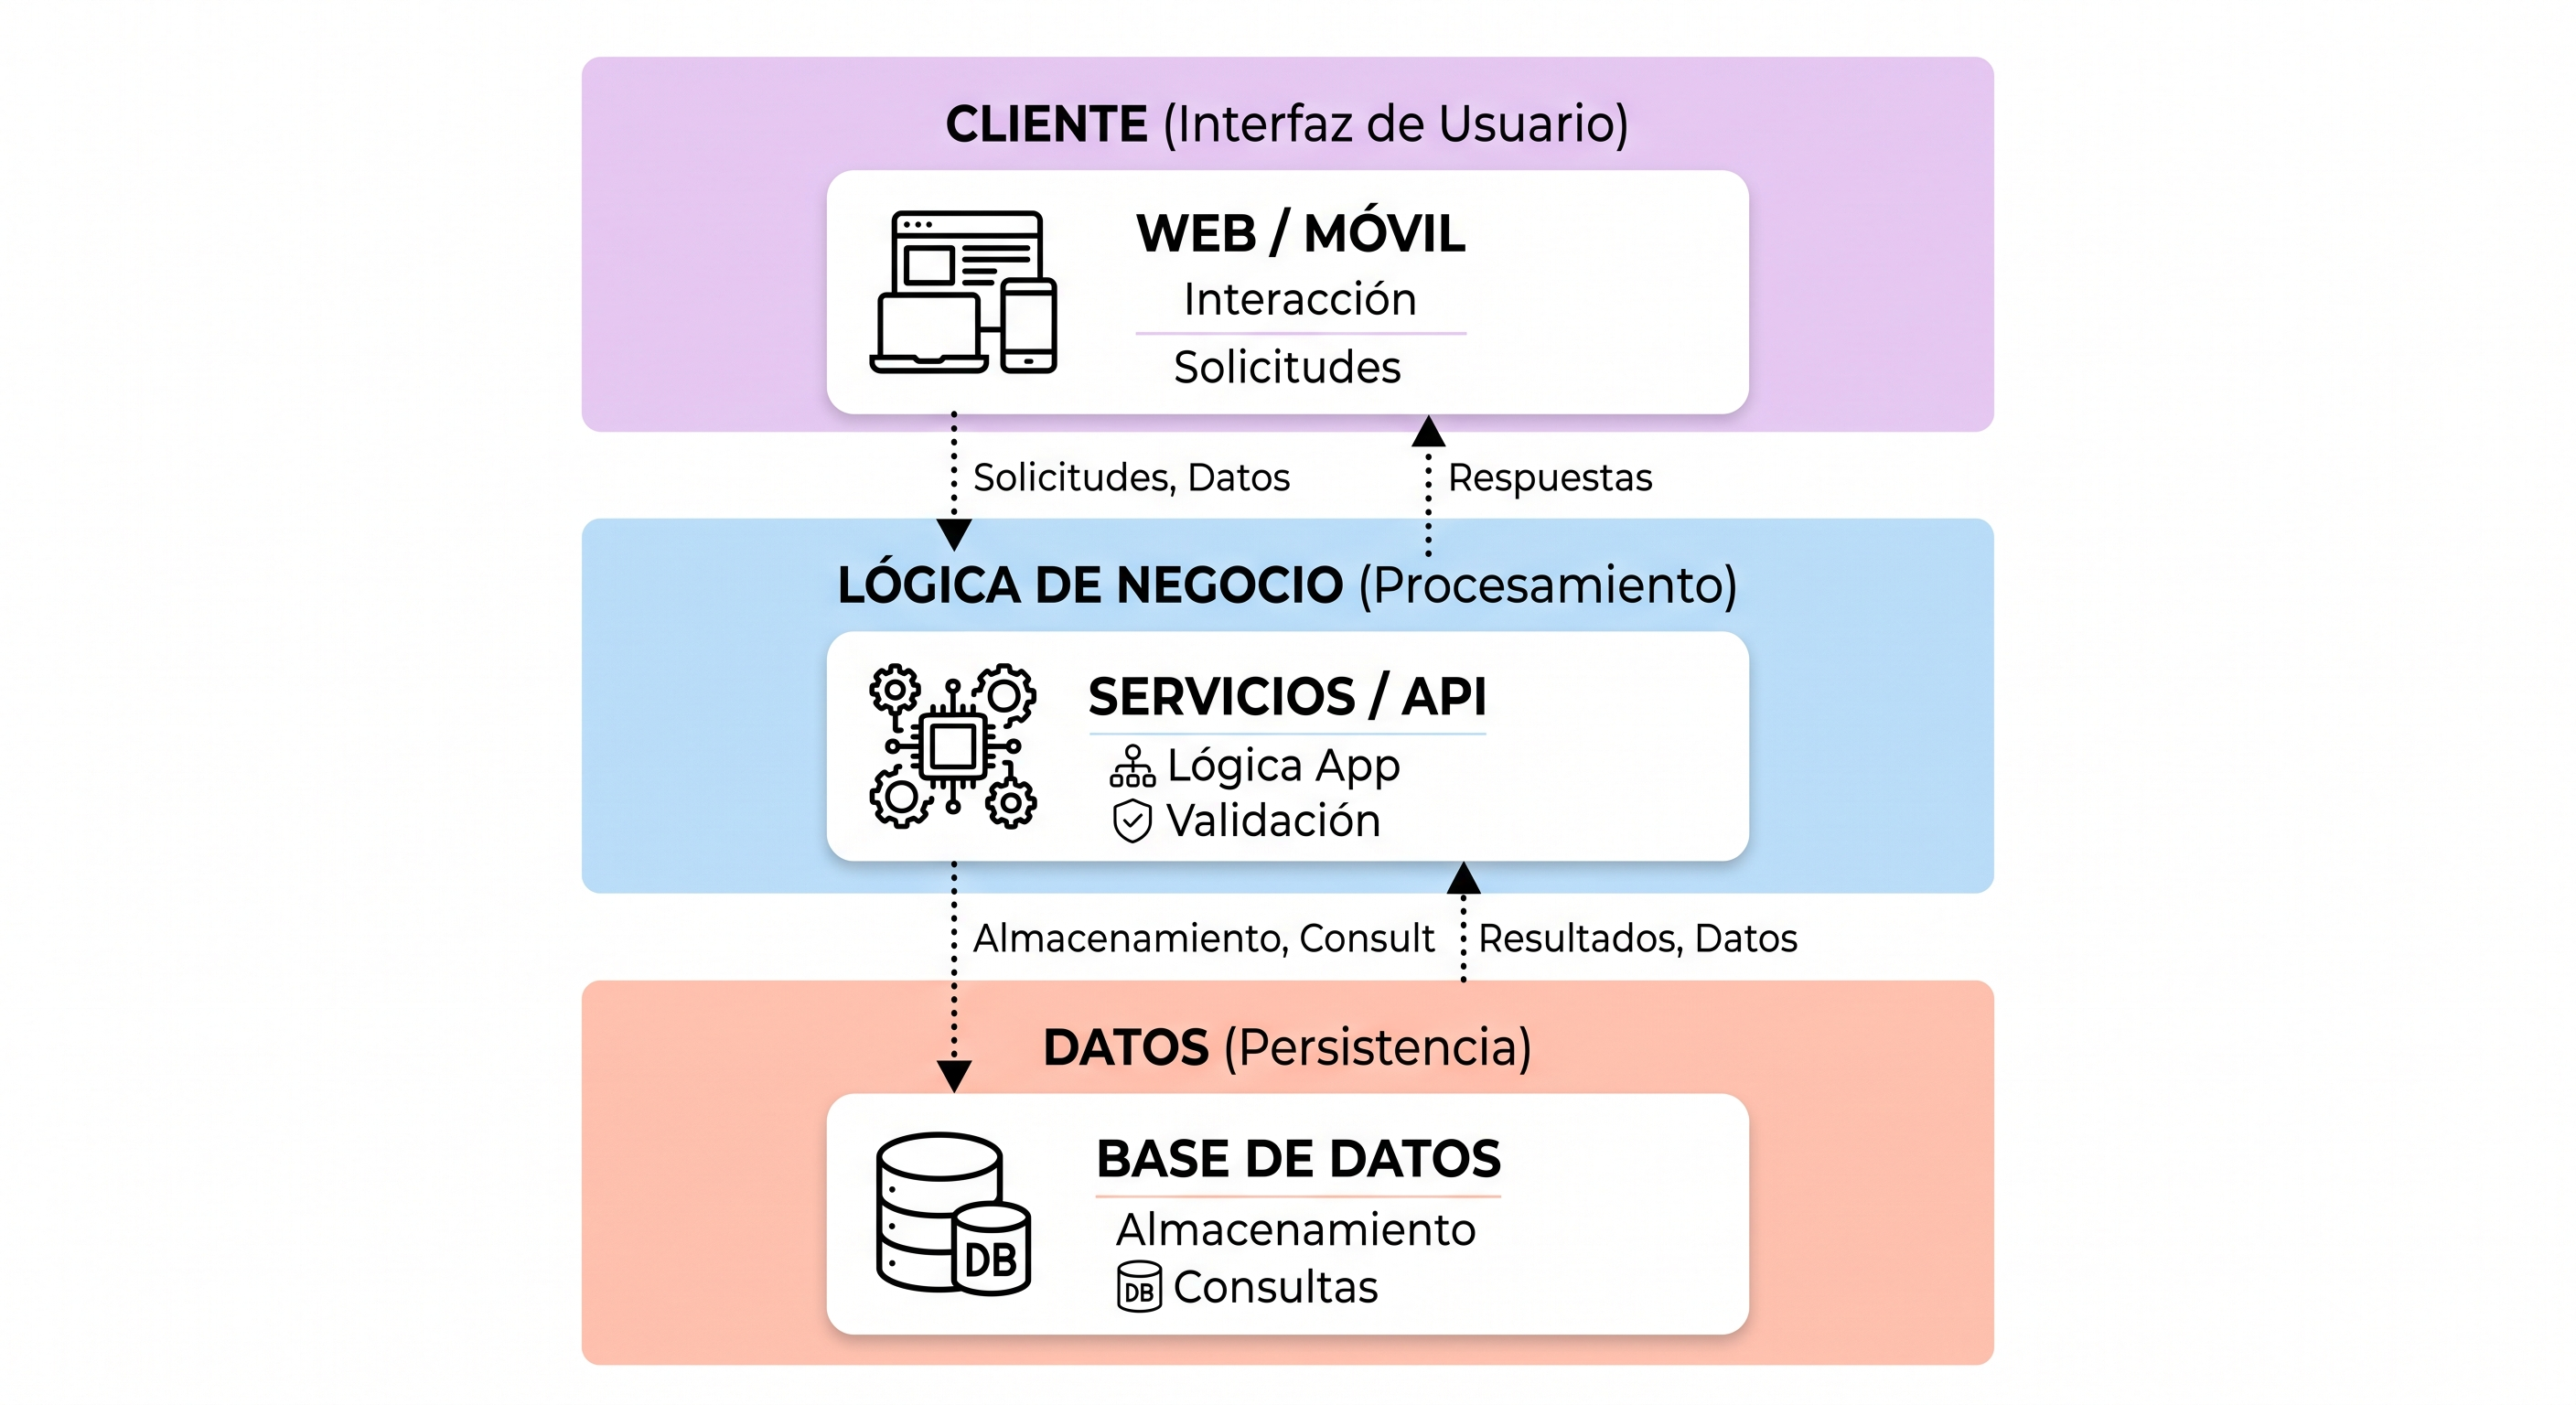
\includegraphics[width=1\textwidth]{Imagenes/arquitectura_capas.jpg} 
    \caption{Representación conceptual de una Arquitectura N-Tier, mostrando el flujo de solicitudes y respuestas entre el Cliente, la Lógica de Negocio (Servicios/API) y la Persistencia de Datos.}
    \label{fig:arquitectura_capas}
\end{diagram}

En la capa de presentación (Cliente), el cambio hacia la portabilidad ha convertido el Diseño Web Responsivo (RWD) en la norma para crear interfaces. Este principio, que fue propuesto por Ethan Marcotte, abandona las dimensiones fijas y se mueve hacia un enfoque flexible que se fundamenta en tres componentes técnicos: rejillas flexibles, imágenes que se ajustan y consultas de medios a través de hojas de estilo en cascada (CSS). \cite{marcotte_rwd_2011}. Las consultas de medios permiten al navegador identificar las dimensiones y características de la pantalla del dispositivo (viewport), reorganizando los elementos visuales de manera dinámica en tiempo real \cite{marcotte_rwd_2011}. Esta capacidad de adaptación no solo evita la necesidad de crear versiones de software separadas para computadoras y teléfonos móviles, sino que también facilita el diseño de interfaces que pueden interactuar de manera nativa con el hardware del dispositivo, como la cámara o el micrófono, usando APIs que están integradas en el navegador \cite{interaccion_nativa_2022}.

En la actualidad, el RWD se apoya en las arquitecturas de Interfaz de Usuario Basadas en Componentes. En este enfoque, las interfaces se desarrollan como un conjunto de fragmentos de código independientes y reutilizables que controlan su propio estado y ciclo de vida \cite{arquitectura_componentes_2021}. Esta modularidad facilita actualizaciones en el navegador de manera reactiva, sin necesidad de recargar toda la página, mejorando así la experiencia del usuario.

La capa de lógica de negocio (Backend) necesita arquitecturas que puedan gestionar múltiples flujos de datos al mismo tiempo. Para apoyar los servicios y APIs, se utilizan entornos de ejecución que son asíncronos y orientados a eventos. Estos entornos permiten que el servidor maneje varias transacciones de red sin que se bloqueen, respondiendo al cliente de forma estructurada y eficiente. \cite{backend_asincrono_2022}.

\paragraph{Persistencia Relacional y Seguridad de la Información} \leavevmode \\

Para asegurar una disposición lógica y una recuperación efectiva de grandes cantidades de información, el modelo de bases de datos relacionales (RDBMS), que fue inicialmente sugerido por Edgar F. Codd, se establece como el estándar clave en el sector del software \cite{Codd1970}. Al contrario de los sistemas de archivos simples, este modelo estructura los datos en grupos de tablas en dos dimensiones, donde cada tabla simboliza una entidad (relación), cada fila tiene un registro singular (tupla) y cada columna especifica una característica particular de dicha entidad \cite{Codd1970}.

La solidez matemática de esta estructura se basa en la normalización y en la aplicación de una integridad referencial rigurosa. Este proceso formal y sistemático tiene como objetivo principal mitigar la redundancia de información y prevenir anomalías lógicas durante las transacciones \cite{silberschatz2014fundamentos}. La normalización se clasifica en diferentes niveles de restricción secuenciales, conocidos como Formas Normales, de las cuales las tres primeras son el estándar de diseño:

\begin{itemize}
    \item \textbf{Primera Forma Normal (1FN):} Establece que el dominio de un atributo debe incluir únicamente valores atómicos (indivisibles), prohibiendo atributos multivaluados o grupos repetitivos dentro de un mismo registro \cite{elmasri2007fundamentos}.
    \item \textbf{Segunda Forma Normal (2FN):} Exige que la tabla cumpla con la 1FN y que todos los atributos no clave dependan en su totalidad de la llave primaria, eliminando las dependencias parciales en llaves compuestas \cite{silberschatz2014fundamentos}.
    \item \textbf{Tercera Forma Normal (3FN):} Dicta que la relación debe cumplir con la 2FN y que ningún atributo no clave dependa transitivamente de la llave primaria, asegurando que dependan exclusivamente de la clave principal \cite{elmasri2007fundamentos}.
\end{itemize}

Mediante el cumplimiento de estas formas y el uso de identificadores únicos que no cambian (llaves primarias) y conexiones lógicas entre diferentes tablas (llaves foráneas), el sistema evita la duplicación de datos y garantiza que las relaciones complejas entre diversas entidades permanezcan coherentes en el esquema topológico \cite{sql_avanzado_2022}.

La orquestación, manipulación y manejo de estas estructuras básicas se realiza a través del Lenguaje de Consulta Estructurado, conocido como SQL. Operativamente, el estándar SQL se subdivide en sublenguajes especializados según su propósito informático \cite{silberschatz2014fundamentos}:

\begin{itemize}
    \item \textbf{Lenguaje de Definición de Datos (DDL):} Es el subconjunto de comandos utilizado estrictamente para declarar y configurar las estructuras lógicas del esquema (como las tablas y llaves).
    \item \textbf{Lenguaje de Manipulación de Datos (DML):} Es el subconjunto algorítmico que permite extraer, inyectar o actualizar las tuplas de información dentro del esquema previamente definido.
\end{itemize}

En situaciones en las que es fundamental la exactitud de los datos operados mediante DML, los motores relacionales realizan lecturas y escrituras siguiendo estrictamente las propiedades transaccionales conocidas como ACID \cite{sql_avanzado_2022}. Estas propiedades establecen que cada transacción debe ser completa e indivisible (Atomicidad), que debe mover la base de datos de un estado correcto a otro (Consistencia), que las transacciones que se realizan al mismo tiempo no deben afectar unas a otras (Aislamiento) y que, después de que se confirme la escritura, la información debe permanecer aún en caso de que ocurra algún problema en el sistema (Durabilidad) \cite{sql_avanzado_2022}. En conjunto, estas garantías evitan que se deterioren los registros almacenados debido a fallos en la red o a cancelaciones inesperadas de las operaciones de guardado.

El manejo de esta persistencia estructural exige fundamentarse en principios estrictos de ciberseguridad, sustentados en los pilares de confidencialidad, integridad y disponibilidad \cite{seguridad_web_oauth_2023}. Para salvaguardar la confidencialidad, los sistemas modernos delegan la autenticación a protocolos de autorización delegada, siendo OAuth 2.0 el framework estándar \cite{seguridad_web_oauth_2023}. El Diagrama \ref{fig:flujo_oauth} detalla el flujo de trabajo de este protocolo mediante la interacción de cuatro entidades: el Propietario, la App Cliente, el Servidor Auth y el Recurso Protegido. Tras el consentimiento del usuario, la aplicación obtiene un código temporal que intercambia por un token criptográfico con el servidor de autorización. El uso de este token final restringe y autentica el acceso a los datos relacionales protegidos, evitando la exposición en texto plano de contraseñas u otras credenciales sensibles \cite{seguridad_web_oauth_2023}.

Mediante este intercambio de tokens, el sistema verifica la identidad del usuario a través de proveedores externos de confianza, evitando la exposición y almacenamiento de contraseñas locales y estableciendo sesiones seguras para el manejo de datos privados \cite{seguridad_web_oauth_2023}.



\begin{diagram}[H]
    \centering
    % Cambia 'ruta_de_tu_imagen_oauth.png' por el nombre y ruta de tu diagrama OAuth
    \includegraphics[width=1\textwidth]{ruta_oauth.jpg} 
    \caption{Diagrama de flujo de autorización OAuth 2.0, mostrando el intercambio seguro de credenciales y tokens criptográficos.}
    \label{fig:flujo_oauth}
\end{diagram}

\subsection{Inteligencia Artificial y Procesamiento de Datos Estructurados}
Una vez que se ha definido la estructura básica del software y los métodos para almacenar datos de forma relacional, el siguiente reto esencial en el diseño de sistemas de información es la recopilación y el entendimiento de datos no organizados. La comunicación humana, ya sea a través de texto libre, lenguaje cotidiano o la digitalización de documentos escritos a mano, es incierta, confusa y no tiene un formato estructurado. Para cerrar la diferencia semántica entre la naturaleza aleatoria de la comunicación humana y la precisión rigurosa de las bases de datos, la ingeniería de software actual utiliza modelos de Inteligencia Artificial. Esta sección proporciona una base teórica sobre las arquitecturas de procesamiento del lenguaje y la inferencia visual, explicando cómo estas tecnologías convierten información sin estructura en variables lógicas organizadas, e introduciendo los métodos de validación humana necesarios para asegurar la integridad, confiabilidad y seguridad de los ecosistemas digitales.
\label{subsec:IA} % Etiqueta en la subsección


\paragraph{Procesamiento de Lenguaje Natural (PLN): De la Sintaxis a la Semántica} \leavevmode \\

El Procesamiento del Lenguaje Natural (PLN) es un campo que combina la informática, la inteligencia artificial y la lingüística computacional. Su finalidad principal es permitir que las computadoras puedan analizar, entender y crear lenguaje humano utilizando algoritmos. En la creación de sistemas interactivos actuales, el PLN actúa como un intermediario entre el lenguaje cotidiano y no estructurado de las personas, y las bases de datos muy organizadas de un sistema informático \cite{jurafsky_nlp_2023}.

La entrada de datos a través de interfaces de texto libre presenta un alto grado de estocasticidad y ruido gramatical. Para que una máquina interprete estas cadenas de caracteres, la información cruda debe someterse a un \textit{pipeline} de preprocesamiento léxico. El Diagrama \ref{fig:pipeline_pln} esquematiza este flujo secuencial, ilustrando cómo un texto de entrada es sistemáticamente depurado a través de tres etapas fundamentales hasta obtener unidades de información matemáticamente procesables.

\begin{diagram}[H]
    \centering
    % Cambia 'ruta_de_tu_imagen_pipeline.png' por el nombre de tu diagrama
    \includegraphics[width=1\textwidth]{pipeline.jpg} 
    \caption{Diagrama de flujo del \textit{pipeline} de preprocesamiento léxico en PLN, demostrando la transformación secuencial desde texto crudo hasta datos tokenizados y lematizados.}
    \label{fig:pipeline_pln}
\end{diagram}

Las técnicas principales que componen este flujo de estandarización son \cite{manning_ir_2008}:

\begin{itemize}[topsep=0pt,itemsep=0pt,parsep=0pt,partopsep=0pt,leftmargin=*]
    \item \textbf{\emph{Tokenización}:} Es el paso inicial de segmentación geométrica. Consiste en dividir una secuencia continua de caracteres en unidades mínimas con significado léxico, denominadas \textit{tokens}. A nivel algorítmico, el sistema identifica delimitadores como espacios en blanco y signos de puntuación, transformando un párrafo continuo en un arreglo dinámico de elementos aislados.
    \item \textbf{Eliminación de palabras vacías (\textit{Stop words}):} Es una técnica de filtrado de ruido. Consiste en descartar términos de altísima frecuencia gramatical (como artículos, preposiciones y conjunciones) que aportan estructura lingüística pero carecen de densidad semántica. Al eliminar estas palabras, el sistema optimiza la carga computacional, conservando únicamente sustantivos, verbos o adjetivos que contienen el valor operativo real de la solicitud.
    \item \textbf{Lematización:} Es el proceso de normalización morfológica. Mediante el uso de diccionarios y análisis gramatical, el algoritmo recorta las terminaciones flexionales (género, número, conjugaciones) para devolver la forma base o de diccionario de una palabra, conocida como \textit{lema}. Por ejemplo, los términos coloquiales 'comprando' o 'compré' son reducidos a su raíz 'comprar', permitiendo que el software agrupe múltiples variaciones bajo un único concepto identificables.
\end{itemize}

Una vez que se ha completado el análisis de la estructura de las oraciones, la comprensión por parte de la computadora debe centrarse en el análisis del significado. Para crear conexiones entre lo que escribe el usuario y las clasificaciones internas del sistema, las estructuras modernas de procesamiento de lenguaje natural dejan de lado las coincidencias básicas de texto (búsquedas precisas) y optan por representaciones vectoriales compactas, llamadas \textit{word embeddings}. \cite{mikolov_word2vec_2013}. 

Esta metodología de aprendizaje profundo asigna cada término del vocabulario a un vector de números reales en un espacio continuo de múltiples dimensiones (espacio latente). En esta forma de representación, se mide la similitud en el significado de manera geométrica al observar lo cerca que están los vectores (normalmente se utiliza la similitud del coseno). Gracias a esto, un sistema informático comprende matemáticamente que palabras diferentes como 'vehículo' y 'automóvil' comparten una equivalencia semántica casi idéntica, permitiendo categorizar solicitudes y asignar códigos estandarizados incluso cuando el usuario utiliza vocabulario informal o sinónimos \cite{jurafsky_nlp_2023}.

%%%%%%%%%%%% 
\paragraph{Extracción de Información (IE) y Reconocimiento de Entidades Nombradas (NER)}\leavevmode \\

Dentro del extenso campo del Procesamiento de Lenguaje Natural, existe una rama sumamente especializada orientada a la estructuración de datos empíricos, conocida como Extracción de Información (IE, por sus siglas en inglés). Se define a la IE como el proceso automatizado de extraer entidades, relaciones y eventos estructurados a partir de fuentes de texto no estructurado \cite{jurafsky_nlp_2023}. Mientras que otras técnicas algorítmicas intentan comprender el sentido global o la intención conversacional de un documento, la IE funciona como un filtro restrictivo: aísla únicamente los datos empíricos que tienen utilidad operativa y descarta el resto del lenguaje natural circundante \cite{grishman_ie_2019}.

Para lograr este nivel de precisión algorítmica en aplicaciones de software comerciales e industriales, los sistemas de extracción dependen de una subtarea técnica fundamental denominada Reconocimiento de Entidades Nombradas (NER, por sus siglas en inglés). Esta tecnología, impulsada fuertemente por arquitecturas de aprendizaje profundo (Deep Learning), permite a una computadora analizar sintaxis compleja para descubrir, delimitar y etiquetar automáticamente palabras clave dentro de un texto, clasificándolas en categorías semánticas predefinidas sin necesidad de intervención manual \cite{li_ner_deep_2020}.

La implementación de modelos NER es un pilar indispensable para automatizar la entrada de datos en sistemas informáticos modernos, dado que el lenguaje utilizado por los usuarios en interfaces de texto libre suele ser desordenado y carente de formato tabular. La Figura \ref{fig:proceso_ner} ilustra la capacidad operativa de esta tecnología para transformar texto bruto en objetos de datos estructurados. 

\begin{figure}[H]
    \centering
    % Cambia 'ruta_de_tu_imagen_ner.png' por el nombre de tu diagrama
    \includegraphics[width=1\textwidth]{ner.jpg} 
    \caption{Esquema conceptual del Reconocimiento de Entidades Nombradas (NER), ilustrando la extracción de entidades discretas y su estructuración en pares clave-valor a partir de un texto libre.}
    \label{fig:proceso_ner}
\end{figure}

A nivel operativo, si un servidor recibe una instrucción cruda como \textit{"Solicito el envío de 50 monitores a la sucursal norte antes del viernes"}, el modelo de red neuronal segmenta la cadena y devuelve etiquetas rigurosamente estructuradas: [Cantidad: 50], [Producto: monitores], [Ubicación: sucursal norte] y [Fecha límite: viernes] \cite{li_ner_deep_2020}. Al transformar párrafos amorfos en variables lógicas independientes y normalizadas, el Reconocimiento de Entidades Nombradas establece los fundamentos técnicos necesarios para poblar bases de datos relacionales, actualizar inventarios y desencadenar eventos en el servidor de manera completamente automatizada.

%%%%%%%%%%
\paragraph{Inferencia Visual Multimodal y Seguridad de Interacción Humana (HITL)} \leavevmode \\

La digitalización de información a partir de documentos físicos o imágenes ha dependido históricamente de las tecnologías de Reconocimiento Óptico de Caracteres (OCR). Si bien esta tecnología es altamente eficiente para transcribir documentos impresos de formato estructurado, presenta deficiencias severas frente a caligrafía humana, ruido visual o formatos inconsistentes \cite{mori_ocr_1992}. La limitación técnica del OCR tradicional radica en su enfoque determinista centrado exclusivamente en la morfología a nivel de caracteres. Los algoritmos clásicos extraen características geométricas (líneas, curvas y bucles) para aislar símbolos individuales dentro de cajas delimitadoras (\textit{bounding boxes}), pero carecen de conocimiento de dominio. En consecuencia, ante la ambigüedad visual de un trazo irregular, el OCR no puede resolver el conflicto, devolviendo cadenas de caracteres ilegibles o sin sentido \cite{smith_tesseract_2007}.

Para superar las limitaciones del análisis morfológico estricto, la inteligencia artificial moderna ha evolucionado hacia los Grandes Modelos de Lenguaje Multimodales (Multimodal LLMs). A diferencia de los modelos de lenguaje tradicionales que solo procesan texto plano, las arquitecturas multimodales integran capas de visión por computadora con transformadores de procesamiento de lenguaje natural \cite{yin_multimodal_2024}. Esta fusión algorítmica permite que el sistema analice una imagen holísticamente, aplicando un razonamiento probabilístico y semántico. Si un modelo multimodal encuentra una palabra físicamente ilegible en un manuscrito, no falla como el OCR, sino que infiere lógicamente el término faltante basándose en el contexto del resto del párrafo, reduciendo drásticamente la tasa de error en la extracción de datos ruidosos \cite{yin_multimodal_2024}.

No obstante, a pesar de su alta capacidad de inferencia, los modelos generativos probabilísticos son susceptibles a un fenómeno algorítmico conocido como \textbf{alucinaciones artificiales}. En el contexto de la extracción de datos, una alucinación ocurre cuando la inteligencia artificial genera o infiere información gramaticalmente coherente y plausible, pero que es fácticamente incorrecta o inexistente en la fuente original \cite{ji_hallucination_2023}. En sistemas de software donde la integridad de los datos es crítica (como inventarios, transacciones financieras o registros legales), una inserción autónoma de datos alucinados en una base de datos relacional representa un riesgo inaceptable de corrupción del sistema.

En el Diagrama \ref{fig:hitl} se muestra como para mitigar esta vulnerabilidad inherente de los modelos generativos, los estándares contemporáneos de ingeniería de software exigen el diseño de arquitecturas con enfoque de "Humano en el bucle" (\textit{Human-in-the-loop} o HITL) \cite{wu_hitl_2022}. Bajo este paradigma de seguridad interactiva, la inteligencia artificial pierde su autonomía de escritura directa. El modelo computacional opera estrictamente como un motor de preprocesamiento, delegando al usuario final la responsabilidad de verificar, auditar y, de ser necesario, corregir las extracciones algorítmicas en la interfaz gráfica antes de que se ejecute la transacción ACID en la base de datos \cite{wu_hitl_2022}. Esta barrera arquitectónica fusiona la velocidad del procesamiento multimodal con la garantía analítica humana, previniendo la persistencia de errores estocásticos.

\begin{diagram}[H]
    \centering
    % Cambia 'ruta_de_tu_imagen_ner.png' por el nombre de tu diagrama
    \includegraphics[width=1\textwidth]{hitl.jpg} 
    \caption{Diagrama que ilustra el diseño de arquitecturas con enfoque de "Humano en el bucle" (\textit{Human-in-the-loop} o HITL).}
    \label{fig:hitl}
\end{diagram}

\paragraph{Interfaces de Voz: Reconocimiento Automático del Habla (ASR) y Síntesis (TTS)}\leavevmode \\

La evolución de la interacción humano-computadora ha trascendido las interfaces gráficas tradicionales para adoptar modalidades acústicas, reduciendo significativamente las barreras de accesibilidad. Esta comunicación bidireccional natural se fundamenta en la integración de dos arquitecturas de inteligencia artificial:

Por un lado, el Reconocimiento Automático del Habla (ASR, por sus siglas en inglés) ejecuta la transcripción de voz a texto. Los algoritmos de ASR capturan ondas sonoras analógicas, las digitalizan y las procesan a través de redes neuronales profundas que analizan espectrogramas para identificar secuencias de fonemas. Estos modelos acústicos están entrenados para mitigar variables de ruido ambiental e inconsistencias de pronunciación, entregando cadenas de texto estructurado que posteriormente son procesadas por los motores de PLN \cite{Yu2014}.

Por otro lado, la Síntesis de Voz (TTS, \textit{Text-to-Speech}) realiza el proceso inverso. A partir de una cadena de caracteres generada por el servidor, el modelo aplica un preprocesamiento de normalización lingüística y modela matemáticamente la prosodia (entonación, ritmo y duración). Finalmente, un vocoder neuronal genera la forma de onda acústica, produciendo habla sintética de alta naturalidad que permite al sistema entregar respuestas dinámicas sin depender de grabaciones preestablecidas \cite{Taylor2009}.

\subsection{Sistemas de Información Geográfica (SIG) y Cartografía Web}

Para extender las capacidades operativas más allá de los datos almacenados localmente, los sistemas de información modernos orquestan hardware, protocolos de red y Sistemas de Información Geográfica (SIG) para proveer Servicios Basados en la Localización (LBS).

\paragraph{Geolocalización, Privacidad y Geocodificación Espacial}\leavevmode \\

El proceso inicial para contextualizar espacialmente a un usuario es la captura algorítmica de su ubicación. En el entorno web, esto se estandariza a través de interfaces de programación integradas en los navegadores (como la \textit{Geolocation API} del W3C). Estas interfaces permiten a la aplicación cliente acceder a las coordenadas espaciales (latitud y longitud) del dispositivo triangulando datos de satélites GPS, redes Wi-Fi cercanas o torres de telecomunicaciones \cite{popescu_geolocation_2016}. Debido a la naturaleza sensible de esta información, la arquitectura web impone un modelo de seguridad estricto que bloquea cualquier rastreo de ubicación por defecto, obligando a que la captura de coordenadas opere exclusivamente bajo el consentimiento explícito y revocable del usuario final \cite{popescu_geolocation_2016}.

Una vez obtenidas las coordenadas matemáticas, los sistemas informáticos requieren traducirlas a formatos legibles para el ser humano o procesables para la lógica de negocio. Este procedimiento se denomina geocodificación. La \textit{geocodificación directa} transforma texto libre (como una dirección postal) en coordenadas espaciales exactas. Por el contrario, la \textit{geocodificación inversa} (\textit{Reverse Geocoding}) toma un par de coordenadas (latitud/longitud) y las mapea contra una base de datos geoespacial para devolver la calle, ciudad o código postal correspondiente \cite{fu_webgis_2010}. Estos algoritmos de traducción bidireccional son el motor lógico que permite al backend calcular distancias, optimizar rutas y ejecutar consultas de proximidad espacial en las bases de datos relacionales.

\paragraph{Arquitectura de Renderizado por Teselas (\textit{Tile-Based Mapping})} \leavevmode \\

Históricamente, la representación gráfica de mapas en aplicaciones web requería que el servidor generara y enviara una imagen monolítica de alta resolución cada vez que el usuario solicitaba una vista, lo que provocaba un consumo insostenible de ancho de banda y una interacción poco fluida. Para resolver este cuello de botella en el rendimiento, la cartografía web moderna adoptó el paradigma de mapas deslizantes (\textit{slippy maps}) basados en sistemas de teselas (\textit{tiles}) \cite{sample_tile_2010}.

Bajo esta arquitectura distribuida, el mapa del mundo no se procesa como un archivo único, sino que se pre-renderiza y fragmenta en una cuadrícula jerárquica de imágenes cuadradas muy ligeras (típicamente de 256x256 píxeles) \cite{sample_tile_2010}. Estas teselas se indexan matemáticamente utilizando un esquema de coordenadas cartesianas XYZ: el nivel de ampliación o \textit{zoom} (Z), la posición horizontal (X) y la posición vertical (Y) \cite{sample_tile_2010}.

Cuando el usuario interactúa con la interfaz de la aplicación (desplazando la pantalla táctil o haciendo \textit{zoom}), la biblioteca gráfica del cliente calcula geométricamente qué teselas específicas entran en el área visible del monitor (\textit{viewport}). A partir de este cálculo, el cliente emite múltiples peticiones HTTP asíncronas únicamente para descargar esos fragmentos necesarios \cite{fu_webgis_2010}. A medida que se reciben, el motor de renderizado del navegador las ensambla en tiempo real formando una cuadrícula continua. 

Sobre esta capa base altamente optimizada, la arquitectura de componentes del cliente permite inyectar información superpuesta. Esto facilita la agregación dinámica de geometría vectorial, polígonos de delimitación o marcadores interactivos para señalar Puntos de Interés (POI), permitiendo a la aplicación modificar el mapa en respuesta a las acciones del usuario sin necesidad de recargar la página completa \cite{fu_webgis_2010}.

\clearpage

\section{Desarrollo del proyecto}
En el desarrollo del BDI se usa una arquitectura modular organizada en tres bloques funcionales: Capa de Datos, Capa de Procesamiento y Lógica y Capa de Visualización. La estructura general del sistema se muestra en el Diagrama~\ref{fig:modulos}. 
{
\begin{diagram}[H] % Ahora sí usamos la H mayúscula para posición fija
	\centering
	\includegraphics[width=1\textwidth]{esquema_bdi.png}
	\caption{\label{fig:modulos} Diagrama de bloques del flujo general del sistema de información.}
\end{diagram}
}

\paragraph{Capa de Datos} \leavevmode \\
Esta capa es la responsable de la recepción, validación, almacenamiento y provisión de la información utilizada por el BDI. Aquí se integra la comunicación con los módulos de la Capa de Procesamiento y Lógica.
\begin{itemize}
        \item Módulo de Control de Datos (CD): Este módulo se encarga de recibir la información ya procesada, validarla y guardarla correctamente con un formato definido. Asimismo, es el responsable de gestionar el aislamiento de la base de datos, actuando como una capa intermedia que impide el acceso directo desde el \emph{frontend} para garantizar la integridad y seguridad de los datos. Además, es el encargado de buscar y entregar los datos rápidamente cuando el sistema o la persona usuaria los solicitan.
        
        \item Base de Datos relacional BDI: Es donde se guarda de forma estructurada toda la información para que el sistema funcione: perfil de la persona usuaria registrada (mediante su cuenta de Google), historial de recetas digitalizadas, el inventario de su botiquín y el diccionario que relaciona los síntomas coloquiales con los términos médicos.
    \end{itemize}

\paragraph{Capa de Procesamiento y Lógica} \leavevmode \\
Esta capa es la responsable de ejecutar la lógica de negocio, centralizar los motores de inteligencia artificial y gestionar la comunicación con servicios de terceros. Su propósito principal es procesar las interacciones provenientes de la Capa de Visualización, transformar la información no estructurada (como fotografías de recetas o síntomas en lenguaje coloquial) en entidades estructuradas, y coordinar su envío seguro hacia la Capa de Datos para su almacenamiento.
\begin{itemize}
        \item Módulo \emph{LLM}: Este módulo es el núcleo analítico del sistema, encargado de procesar las fotografías de las recetas médicas impresas o manuscritas y de las cajas o etiquetas de los medicamentos. Para su implementación, se desarrolló una estrategia multimodelo (\emph{Adapter Pattern}) que emplea Google Gemini Flash Lite \cite{geminiapi} como motor principal y Qwen3.8-27B (accesible mediante la API de Groq \cite{CostoGroq}) como modelo de contingencia o balanceo. El módulo recibe como entrada (datos de entrada) la fotografía optimizada y codificada en formato Base64 junto con un \emph{prompt} de sistema estructurado, y devuelve como salida un objeto estandarizado en formato JSON de manera resiliente, logrando filtrar alucinaciones residuales de texto mediante un parser defensivo. Su función principal es extraer de forma automática las siguientes entidades:
        \begin{itemize}
            \item En el caso de recetas médicas: nombre, fecha, cédula profesional del personal médico, diagnóstico, nombres de medicamentos recetados e indicaciones para construir el historial clínico.
            \item En el caso de medicamentos: capturar el nombre, dosis y fecha de caducidad para alertar a la persona usuaria sobre si un fármaco está vigente, próximo a vencer o ya ha caducado.
        \end{itemize}

        Para manejar posibles alucinaciones de la inteligencia artificial, respuestas incorrectas o imágenes con baja resolución, el sistema implementa un mecanismo de validación en la interfaz (\emph{Human-in-the-loop}). Antes de insertar la salida del modelo en la base de datos, la información se presenta en un formulario web editable donde la persona usuaria debe revisar, corregir y confirmar los datos extraídos por el LLM. Además, como estrategia de contingencia, si el modelo falla al extraer la información, se habilita la opción de captura manual total.
        
        \item Módulo ubicación de farmacias: Este módulo se encarga de procesar la información geográfica del dispositivo, tomando la ubicación en tiempo real de la persona usuaria o una dirección ingresada manualmente para mostrar un mapa interactivo con las farmacias más cercanas, facilitando la adquisición del medicamento.

        \item Módulo de consulta de precios: Este módulo tiene la tarea de realizar búsquedas para recopilar costos actualizados de los medicamentos en diferentes establecimientos. Esto permite a la persona usuaria visualizar rápidamente las opciones más económicas antes de realizar una compra.

        \item Módulo voz-texto y texto-voz: Este módulo procesa el audio capturado por el micrófono del dispositivo para transformarlo en texto escrito, permitiendo a la persona usuaria describir un síntoma sin necesidad de teclear; también puede tomar el texto de los resultados y reproducirlo en audio a través de los altavoces. Esto mejora la accesibilidad y experiencia en el BDI. 

        \item Módulo términos coloquiales a técnicos: Este módulo procesa síntomas ingresados por la persona usuaria que utilicen términos coloquiales y los mapea a términos médicos oficiales CIE-10 \cite{CIE10}. Esto permite que el sistema busque en el historial de recetas del usuario qué tratamiento le ha sido prescrito anteriormente para esa condición específica.   
    \end{itemize}
    
\paragraph{Capa de Visualización} \leavevmode \\
Esta capa representa la interfaz web con la que interactúa la comunidad usuaria.
\begin{itemize}
    \item Interfaz: Permite a la persona usuaria autenticarse mediante su cuenta de Google, garantizando el acceso desde cualquier dispositivo a su botiquín e historial médico. Además, agrupa todos los servicios del BDI como ingresar texto, dictar síntomas por voz y recuperar el historial de recetas, presentar el mapa dinámico para la localización de farmacias cercanas y mostrar tablas de comparación de precios, haciendo la interacción amigable, intuitiva y fácil de entender.
    \item Módulo de captura de fotografías: Este módulo se encarga de solicitar los permisos necesarios al dispositivo para acceder a la cámara o galería. Su función es permitir a la persona usuaria capturar y confirmar las fotografías de sus recetas o cajas de medicamentos para su posterior procesamiento.
\end{itemize}

\subsection{Capa de Datos}

La Capa de Datos del Botiquín Digital Inteligente (BDI) es la responsable de la recepción, validación, almacenamiento y provisión de la información médica sensible. Para cumplir con los requisitos de consistencia y concurrencia, esta capa se diseñó bajo un modelo de bases de datos relacionales, implementando un Módulo de Control de Datos que actúa como intermediario seguro entre la lógica de negocio y la persistencia física.

\subsubsection{Diseño del Esquema Relacional de Base de Datos}

% Propuesta detallada y extendida para añadir en la sección \subsubsection{Diseño del Esquema Relacional de Base de Datos}
% Incluye tablas visuales y justificación exhaustiva de la metodología.

La construcción y definición de la base de datos se llevó a cabo siguiendo una rigurosa metodología de diseño relacional por fases. Este proceso, que partió desde la abstracción de las reglas de negocio hasta la validación empírica de las formas normales, se detalla exhaustivamente a continuación:

\paragraph{1. Descripción del Problema y Extracción de Sustantivos (Identificación de Entidades)} \leavevmode \\

El diseño de la arquitectura de datos inició con un análisis exhaustivo del contexto y los requerimientos funcionales del Botiquín Digital Inteligente (BDI). Al diseccionar la descripción de las operaciones requeridas (digitalización de recetas médicas, gestión del inventario físico, traducción de síntomas y notificaciones), se aplicó la técnica de extracción de sustantivos. Esta técnica consistió en identificar todos los nombres sustantivos presentes en la lógica del negocio y someterlos a un proceso de filtrado para distinguir cuáles representarían entidades fundamentales, cuáles serían simples atributos, y cuáles eran redundancias (sinónimos). 

La Tabla \ref{tab:extraccion_sustantivos} muestra el resultado de este proceso analítico.

\begin{longtable}{|p{0.3\textwidth}|p{0.25\textwidth}|p{0.4\textwidth}|}
\caption{Proceso de Extracción y Clasificación de Sustantivos.}
\label{tab:extraccion_sustantivos} \\
\hline
\textbf{Sustantivo Extraído} & \textbf{Clasificación} & \textbf{Justificación / Decisión} \\
\hline
\endfirsthead
\hline
\textbf{Sustantivo Extraído} & \textbf{Clasificación} & \textbf{Justificación / Decisión} \\
\hline
\endhead
\hline
\endfoot
\hline
\endlastfoot
Paciente / Usuario & Entidad & Se consolidan como la entidad \texttt{Usuarios}. \\
\hline
Médico / Doctor & Entidad & Se consolida como la entidad \texttt{Medicos}. \\
\hline
Receta Médica & Entidad & Entidad transaccional \texttt{Recetas}. \\
\hline
Medicamento / Fármaco & Entidad & Catálogo maestro \texttt{Catalogo\_Medicamentos}. \\
\hline
Botiquín / Inventario & Entidad & Representa el stock físico \texttt{Botiquin}. \\
\hline
Diagnóstico CIE-10 & Entidad & Diccionario médico \texttt{Catalogo\_CIE10}. \\
\hline
Recordatorio / Alarma & Entidad & Sistema de notificaciones \texttt{Recordatorios}. \\
\hline
Correo Electrónico & Atributo & Propiedad de la entidad \texttt{Usuarios}. \\
\hline
Dosis / Frecuencia & Atributo & Propiedad del cruce entre Receta y Medicamento. \\
\hline
Síntoma coloquial & Atributo & Propiedad (arreglo JSON) del \texttt{Catalogo\_CIE10}. \\
\hline
Búsqueda de precios & Entidad & Transaccional \texttt{Busquedas\_Precios}. \\
\hline
Suscripción / Dispositivo & Entidad & Notificaciones \texttt{Suscripciones\_Push}. \\
\hline
Toma diaria / Consumo & Entidad & Seguimiento \texttt{Tomas\_Diarias}. \\
\hline
\end{longtable}

\paragraph{2. Definición de Atributos y Relaciones entre Entidades} \leavevmode \\

Tras aislar las entidades base, se procedió a definir su diccionario de datos preliminar (sus atributos característicos) y a trazar la cardinalidad de sus interacciones lógicas. Las reglas de negocio dictaron flujos específicos: un usuario posee un botiquín, un médico expide múltiples recetas, y una receta abarca varios medicamentos. 

La Tabla \ref{tab:atributos_entidades} resume los atributos asignados, mientras que la Tabla \ref{tab:matriz_relaciones} expone la matriz de cardinalidad geométrica entre los componentes.

\begin{longtable}{|p{0.25\textwidth}|p{0.7\textwidth}|}
\caption{Diccionario de Datos Preliminar (Atributos por Entidad).}
\label{tab:atributos_entidades} \\
\hline
\textbf{Entidad} & \textbf{Atributos Principales} \\
\hline
\endfirsthead
\hline
\textbf{Entidad} & \textbf{Atributos Principales} \\
\hline
\endhead
\hline
\endfoot
\hline
\endlastfoot
\texttt{Usuarios} & identificador, nombre, correo\_electronico, google\_id. \\
\hline
\texttt{Medicos} & identificador, nombre\_completo, cedula\_profesional, especialidad. \\
\hline
\texttt{Recetas} & identificador, fecha\_expedicion, diagnostico, url\_fotografia. \\
\hline
\texttt{Catalogo\_Medicamentos}& identificador, nombre\_comercial, sustancia\_activa, presentacion. \\
\hline
\texttt{Botiquin} & identificador, cantidad\_disponible, fecha\_caducidad, unidad. \\
\hline
\texttt{Recordatorios} & identificador, fecha\_inicio, frecuencia\_horas, estado\_activo. \\
\hline
\texttt{Catalogo\_CIE10} & identificador, codigo\_oms, descripcion, keywords\_json. \\
\hline
\texttt{Busquedas\_Precios} & identificador, id\_medicamento, resultados\_json, fecha\_busqueda. \\
\hline
\texttt{Suscripciones\_Push} & identificador, id\_usuario, endpoint, p256dh\_key, auth\_key. \\
\hline
\texttt{Tomas\_Diarias} & identificador, id\_recordatorio, id\_usuario, fecha\_hora, estado. \\
\hline
\texttt{Recetas\_Detalles} & identificador, id\_receta, id\_catalogo, dosis, frecuencia, duracion. \\
\hline
\end{longtable}

\begin{longtable}{|p{0.25\textwidth}|p{0.2\textwidth}|p{0.25\textwidth}|p{0.2\textwidth}|}
\caption{Matriz de Relaciones y Cardinalidad.}
\label{tab:matriz_relaciones} \\
\hline
\textbf{Entidad Origen} & \textbf{Verbo} & \textbf{Entidad Destino} & \textbf{Cardinalidad} \\
\hline
\endfirsthead
\hline
\textbf{Entidad Origen} & \textbf{Verbo} & \textbf{Entidad Destino} & \textbf{Cardinalidad} \\
\hline
\endhead
\hline
\endfoot
\hline
\endlastfoot
\texttt{Usuarios} & gestiona & \texttt{Botiquin} & 1 : N \\
\hline
\texttt{Usuarios} & recibe & \texttt{Recetas} & 1 : N \\
\hline
\texttt{Medicos} & prescribe & \texttt{Recetas} & 1 : N \\
\hline
\texttt{Recetas} & contiene & \texttt{Catalogo\_Med.} & N : M \\
\hline
\texttt{Botiquin} & requiere & \texttt{Recordatorios} & 1 : N \\
\hline
\texttt{Recetas} & asocia & \texttt{Catalogo\_CIE10} & N : 1 \\
\hline
\texttt{Usuarios} & habilita & \texttt{Suscripciones\_Push} & 1 : N \\
\hline
\texttt{Catalogo\_Med.} & cotiza & \texttt{Busquedas\_Precios} & 1 : N \\
\hline
\texttt{Recordatorios} & genera & \texttt{Tomas\_Diarias} & 1 : N \\
\hline
\end{longtable}

\paragraph{3. Identificación de Llaves Primarias, Foráneas y Tablas Puente} \leavevmode \\

Con el esqueleto lógico definido, se implementó la arquitectura de llaves para habilitar la trazabilidad referencial. Se asignó una Llave Primaria (\textit{Primary Key}) autoincrementable y numérica a cada entidad para optimizar la indexación de los árboles de búsqueda.

Un hito crucial en esta etapa fue la resolución de las relaciones de muchos a muchos (N:M). Como se evidenció en la matriz de relaciones, \texttt{Recetas} y \texttt{Catalogo\_Medicamentos} mantienen una cardinalidad N:M. Para normalizar esto, se diseñó la tabla puente \texttt{Recetas\_Detalles}. Esta tabla no solo almacena las llaves foráneas de ambas entidades, sino que captura los atributos que \textbf{exclusivamente existen cuando ambas interactúan} (dosis y frecuencia). La Tabla \ref{tab:llaves_tablas_puente} ilustra el diseño de estas tablas asociativas.

\begin{longtable}{|p{0.25\textwidth}|p{0.3\textwidth}|p{0.4\textwidth}|}
\caption{Diseño de Tablas Puente para Resolución de Relaciones N:M.}
\label{tab:llaves_tablas_puente} \\
\hline
\textbf{Tabla Puente} & \textbf{Llaves Foráneas (Unen a:)} & \textbf{Atributos Propios de la Interacción} \\
\hline
\endfirsthead
\hline
\textbf{Tabla Puente} & \textbf{Llaves Foráneas (Unen a:)} & \textbf{Atributos Propios de la Interacción} \\
\hline
\endhead
\hline
\endfoot
\hline
\endlastfoot
\texttt{Recetas\_Detalles} & \texttt{id\_receta}, \texttt{id\_catalogo} & dosis, frecuencia\_horas, duracion\_dias, indicaciones\_extra. \\
\hline
\texttt{Tomas\_Diarias} & \texttt{id\_recordatorio}, \texttt{id\_usuario} & fecha\_hora\_programada, estado\_toma (completado/omitido). \\
\hline
\end{longtable}

Como regla de integridad, todas las llaves foráneas ligadas a \texttt{Usuarios} fueron configuradas con la restricción \texttt{ON DELETE CASCADE}, delegando al motor MySQL la limpieza absoluta de los datos si un usuario elimina su cuenta.

\paragraph{4. Justificación Empírica del Proceso de Normalización} \leavevmode \\

Para garantizar la coherencia absoluta de los datos clínicos y prevenir anomalías, se estructuró la base de datos hasta la \textbf{Tercera Forma Normal (3FN)}. A continuación, se justifica este proceso visualmente mediante extractos de registros reales del sistema:

\subparagraph{Primera Forma Normal (1FN): Atributos Atómicos} \leavevmode \\
La 1FN exige que no haya grupos repetitivos ni atributos multivaluados. En el diseño del BDI, una receta \textbf{no} guarda todos sus medicamentos en una sola celda separada por comas. Como se observa en la Tabla \ref{tab:ejemplo_recetas_detalles}, cada medicamento recetado ocupa un registro independiente y atómico en la tabla puente.

\begin{longtable}{|c|c|c|c|c|}
\caption{Extracto de la tabla \texttt{Recetas\_Detalles} demostrando el cumplimiento de la 1FN.}
\label{tab:ejemplo_recetas_detalles} \\
\hline
\textbf{id\_detalle} & \textbf{id\_receta} & \textbf{id\_catalogo} & \textbf{dosis} & \textbf{frecuencia\_horas} \\
\hline
\endfirsthead
\hline
\textbf{id\_detalle} & \textbf{id\_receta} & \textbf{id\_catalogo} & \textbf{dosis} & \textbf{frecuencia\_horas} \\
\hline
\endhead
\hline
\endfoot
\hline
\endlastfoot
1 & 100 & 5 (Paracetamol) & 500mg & 8 \\
\hline
2 & 100 & 12 (Amoxicilina) & 250mg & 12 \\
\hline
3 & 101 & 5 (Paracetamol) & 500mg & 8 \\
\hline
\end{longtable}

\subparagraph{Segunda Forma Normal (2FN): Sin Dependencias Parciales} \leavevmode \\
La 2FN establece que todos los atributos no clave deben depender por completo de la llave primaria. En la Tabla \ref{tab:ejemplo_recetas_detalles}, atributos como \texttt{dosis} y \texttt{frecuencia\_horas} no dependen solo de la receta, ni dependen solo del medicamento; dependen de la combinación íntegra de \texttt{id\_receta} y \texttt{id\_catalogo}. Si un atributo dependiera solo del medicamento (como su vía de administración genérica), violaría la 2FN y debería ir en el catálogo maestro.

\subparagraph{Tercera Forma Normal (3FN): Sin Dependencias Transitivas} \leavevmode \\
La 3FN prohíbe que atributos no clave dependan de otros atributos no clave. En el diseño inicial, se podría haber cometido el error de almacenar el nombre del médico directamente en la tabla de \texttt{Recetas}. Sin embargo, el nombre del médico depende de la \texttt{cedula\_profesional}, lo que crearía una dependencia transitiva. Para cumplir la 3FN, los datos del médico se aislaron en la tabla \texttt{Medicos} (Tabla \ref{tab:ejemplo_medicos}), y la tabla \texttt{Recetas} (Tabla \ref{tab:ejemplo_recetas}) únicamente guarda la llave foránea \texttt{id\_medico}.

\begin{longtable}{|c|c|l|c|}
\caption{Extracto de la tabla \texttt{Medicos} (Aislada por 3FN).}
\label{tab:ejemplo_medicos} \\
\hline
\textbf{id\_medico} & \textbf{nombre\_completo} & \textbf{cedula\_profesional} & \textbf{especialidad} \\
\hline
\endfirsthead
\hline
\textbf{id\_medico} & \textbf{nombre\_completo} & \textbf{cedula\_profesional} & \textbf{especialidad} \\
\hline
\endhead
\hline
\endfoot
\hline
\endlastfoot
1 & Dr. Roberto Gómez & 7654321 & Medicina General \\
\hline
2 & Dra. Silvia Méndez & 9876543 & Pediatría \\
\hline
\end{longtable}

\begin{longtable}{|c|c|c|c|l|}
\caption{Extracto de la tabla \texttt{Recetas} (Relacionada por Llave Foránea).}
\label{tab:ejemplo_recetas} \\
\hline
\textbf{id\_receta} & \textbf{id\_usuario} & \textbf{id\_medico} & \textbf{fecha\_expedicion} & \textbf{diagnostico} \\
\hline
\endfirsthead
\hline
\textbf{id\_receta} & \textbf{id\_usuario} & \textbf{id\_medico} & \textbf{fecha\_expedicion} & \textbf{diagnostico} \\
\hline
\endhead
\hline
\endfoot
\hline
\endlastfoot
100 & 10 & \textbf{1} & 2024-03-15 & Faringitis aguda \\
\hline
101 & 15 & \textbf{2} & 2024-03-16 & Infección viral \\
\hline
102 & 10 & \textbf{1} & 2024-04-01 & Gastritis \\
\hline
\end{longtable}

Esta arquitectura normalizada elimina las anomalías de actualización; si el Dr. Roberto Gómez cambia de consultorio o actualiza su especialidad, el sistema BDI únicamente modifica una fila en la tabla \texttt{Medicos}, y automáticamente todas las recetas históricas asociadas a él reflejan la actualización, garantizando la consistencia global.

Para el almacenamiento estructurado de la información, se configuró un servidor de bases de datos utilizando el motor \emph{MySQL}. El diseño de este modelo relacional fue fundamental para garantizar la integridad de los datos clínicos.

En el Diagrama~\ref{dia:der_mysql} se ilustra visualmente la estructura de estas entidades y sus relaciones.

\begin{diagram}[H]
\centering
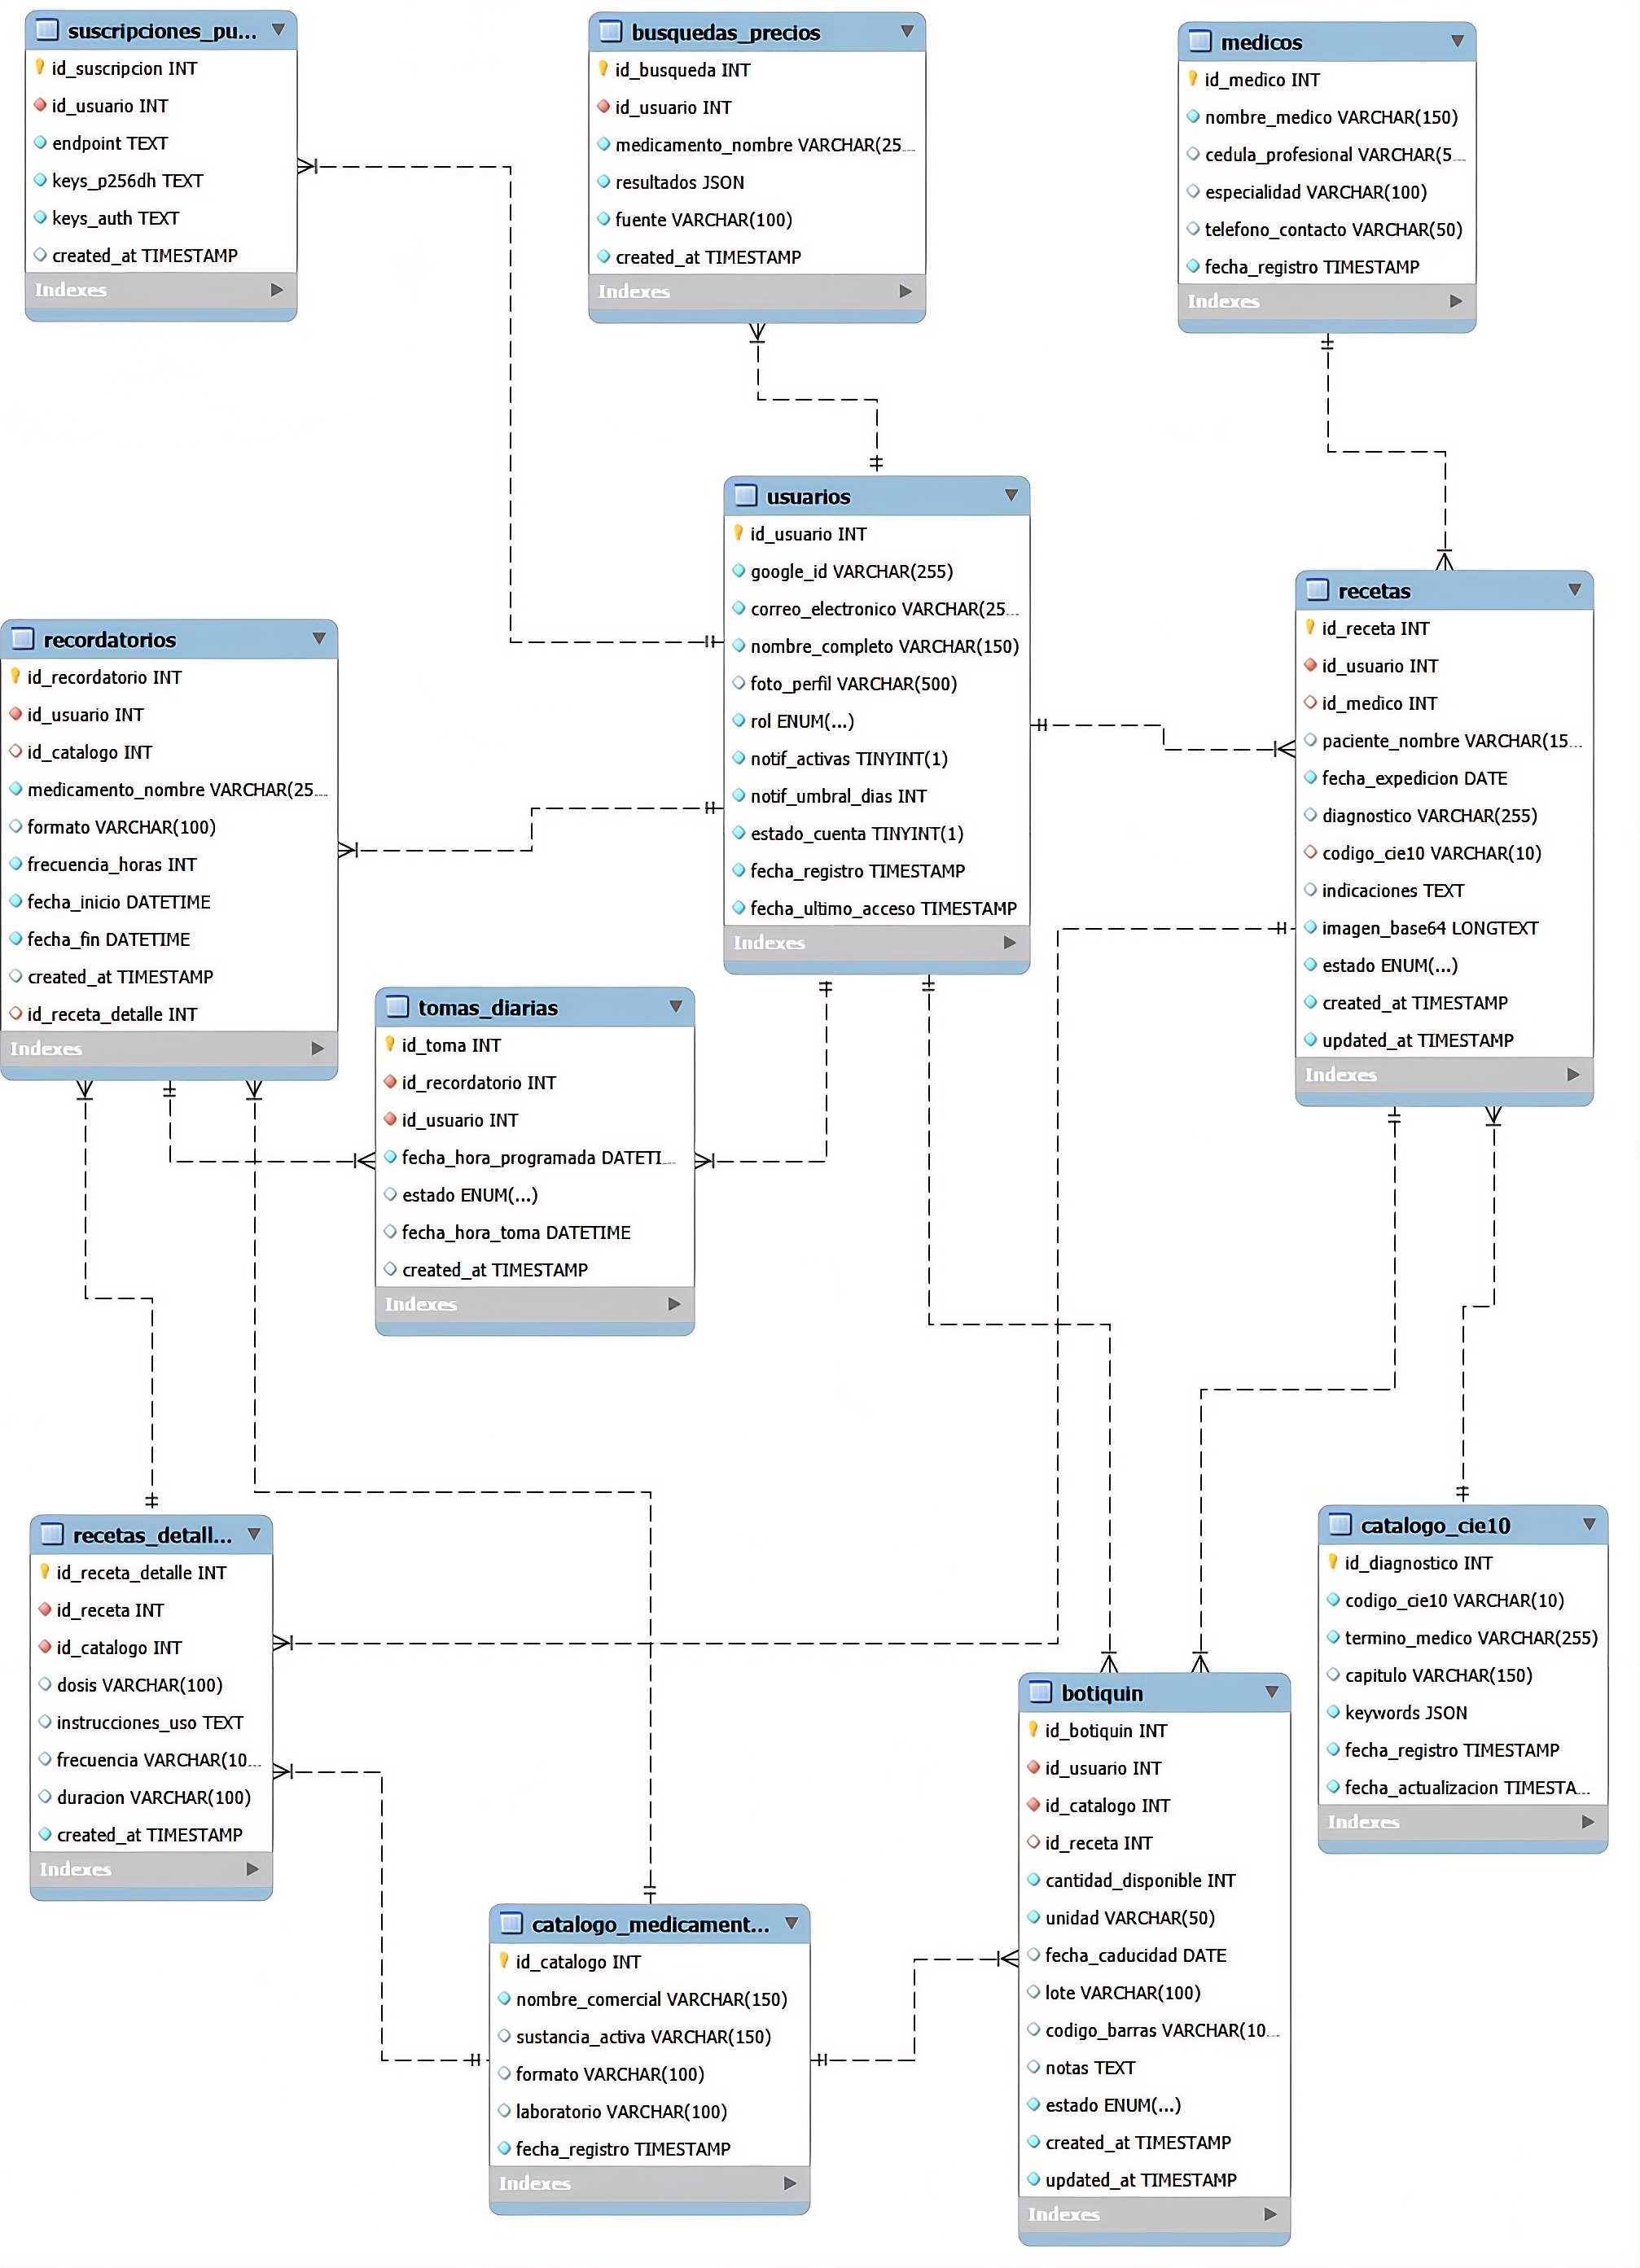
\includegraphics[width=0.97\textwidth]{Imagenes/entidad_relacion_bd.png}
\caption{Diagrama Entidad-Relación (DER) del sistema BDI ilustrando las relaciones entre las once entidades.}
\label{dia:der_mysql}
\end{diagram}

\paragraph{5. Generación de Lenguaje de Manipulación de Datos (DML) para el Catálogo CIE-10} \leavevmode \\

Una de las piezas centrales del proyecto es la capacidad de mapear el lenguaje médico estandarizado con el vocabulario común de los usuarios. Para lograr esto, la entidad \texttt{Catalogo\_CIE10} no podía ser poblada manualmente debido a la magnitud de los términos médicos y la inmensa cantidad de variantes coloquiales. Por lo tanto, el Lenguaje de Manipulación de Datos (DML) para esta tabla, compuesto fundamentalmente por sentencias \texttt{INSERT INTO}, fue automatizado apoyándose en Inteligencia Artificial.

Se desarrolló un \textit{script} en Python (\texttt{generar\_inserts\_ia.py}) encargado de orquestar esta labor. Para obtener el compendio médico oficial, se descargó el catálogo tabular de la Clasificación Internacional de Enfermedades (CIE-10) directamente desde los repositorios de las autoridades de salud \cite{CIE10}. Una vez limpiado el formato original, este módulo toma como base los códigos y descripciones extraídos y, a través de la integración con modelos de lenguaje multimodales (LLM), genera dinámicamente un arreglo de \textit{keywords} (sinónimos o formas coloquiales en las que una persona sin formación médica describiría dicha enfermedad, por ejemplo: "me duele la cabeza" para el código R51). 

Posteriormente, el programa formatea esta información y construye y ejecuta las sentencias SQL parametrizadas, encapsulando los síntomas coloquiales dentro del atributo nativo \texttt{JSON}. Como se puede observar detalladamente en el Código \ref{lst:dml_cie10}, el sistema facilita la elaboración del registro combinando la precisión de la nomenclatura oficial con la variedad del lenguaje cotidiano. \\

\begin{lstlisting}[language=SQL, caption={Ejemplo de sentencia DML (INSERT INTO) generada algorítmicamente mediante IA para poblar la entidad \texttt{Catalogo\_CIE10}.}, label={lst:dml_cie10}]
INSERT INTO catalogo_cie10 (codigo_oms, descripcion, keywords_json) 
VALUES (
    'J00', 
    'Rinofaringitis aguda (resfriado comun)', 
    '["gripa", "catarro", "moco", "cuerpo cortado", "me duele la garganta"]'
);
\end{lstlisting}

Esta estrategia de DML asistido por IA garantizó la inserción masiva y estructurada del catálogo, dotando al motor de base de datos del contexto semántico necesario para que las búsquedas operen de forma eficiente cuando el usuario ingresa sus síntomas en lenguaje natural.

\subsubsection{Módulo de Control de Datos (CD) y Seguridad}

El desarrollo de este módulo se enfocó en la programación del entorno de \emph{backend} (\emph{Node.js} y \emph{Express.js}). Para establecer la comunicación directa y asíncrona con \emph{MySQL}, se integró la librería \texttt{mysql2/promise}.

\paragraph{Validación de datos con Zod}\leavevmode \\
Para proteger la base de datos contra inyecciones e información inconsistente, se programaron \emph{middlewares} de protección apoyados en la biblioteca \textbf{Zod}. Estas funciones interceptan el cuerpo de la petición (JSON) y validan rigurosamente que cada propiedad cumpla con los tipos de datos y expresiones regulares permitidos antes de ejecutar cualquier sentencia \texttt{INSERT} o \texttt{UPDATE}. Como se ilustra en el Código \ref{lst:zod_schema}, esta validación define reglas estrictas para cada campo del botiquín, asegurando que valores críticos como el ID del catálogo o la cantidad disponible sean siempre números enteros positivos, y verificando que la fecha de caducidad respete el formato estándar \texttt{YYYY-MM-DD}. \\

\begin{lstlisting}[language=JavaScript, caption={Esquema de validación implementado con Zod para asegurar la integridad de los registros del botiquín.}, label={lst:zod_schema}]
const inventarioSchema = z.object({
  id_catalogo: z.number().int().min(1, 'El ID de catálogo es obligatorio'),
  cantidad_disponible: z.number().int().min(0, 'La cantidad debe ser 0 o mayor'),
  unidad: z.string().min(1, 'La unidad es obligatoria'),
  fecha_caducidad: z.string().regex(/^\d{4}-\d{2}-\d{2}$/, 'Formato inválido (YYYY-MM-DD)')
});
\end{lstlisting}


\paragraph{Lógica de Control de Caducidad} \leavevmode \\
Una de las funcionalidades desarrolladas fue el control del estado del medicamento. Aprovechando el formato estricto ISO 8601 (\texttt{YYYY-MM-DD}) de la \texttt{fecha\_caducidad}, el controlador ejecuta una lógica de comparación de fechas utilizando funciones nativas de \emph{JavaScript} (\texttt{new Date()}) y sentencias \texttt{DATEDIFF} de SQL. Esto permite clasificar dinámicamente cada fármaco como 'vigente', 'por vencer' (si restan menos de 30 días) o 'caducado', permitiendo a la capa visual alertar al paciente oportunamente.

\paragraph{Autenticación JSON Web Tokens (JWT)} \leavevmode \\
El aislamiento de los datos se rige por un esquema de autenticación basado en \emph{Google OAuth2} y \emph{JWT}. Cuando el usuario inicia sesión mediante la ruta \texttt{POST /api/auth/google}, el servidor utiliza \texttt{google-auth-library} para validar el criptograma. Una vez autenticado de forma exitosa, emite un token local firmado.

Las rutas que exigen protección a la información clínica (como agregar o leer recetas) están envueltas por el \emph{middleware} de seguridad \texttt{verifyToken}, el cual decodifica la identidad y la inyecta globalmente (\texttt{req.usuario = decoded}). Este mecanismo, detallado en el Código \ref{lst:verify_jwt}, intercepta la cabecera HTTP de autorización para extraer el token y verificar su criptograma mediante una clave secreta; si el token resulta inválido o ha expirado, la solicitud se rechaza automáticamente con un error 403, protegiendo así las rutas sensibles. \\

\begin{lstlisting}[language=JavaScript, caption={Middleware de seguridad para la validación de JSON Web Tokens en rutas protegidas.}, label={lst:verify_jwt}]
const verifyToken = (req, res, next) => {
  const authHeader = req.headers['authorization'];
  const token = authHeader && authHeader.split(' ')[1];
  
  if (!token) return res.status(401).json({ error: 'Acceso denegado' });

  try {
    const decoded = jwt.verify(token, process.env.JWT_SECRET);
    req.usuario = decoded; // Inyección de identidad global
    next();
  } catch (error) {
    return res.status(403).json({ error: 'Token inválido o expirado' });
  }
};
\end{lstlisting}

Para evitar vulnerabilidades de suplantación de identidad en las consultas, en cada operación SQL que afecte datos privados se concatena explícitamente el identificador de la sesión actual (por ejemplo: \texttt{WHERE id\_usuario = ?}).

\subsubsection{Organización de Endpoints RESTful}

La comunicación del \emph{backend} se diseñó bajo una arquitectura basada en rutas (\emph{routes}) organizadas por entidades lógicas, cada una dedicada a un servicio específico del botiquín digital. En la Tabla \ref{tab:endpoints_db} se presenta un extracto de los principales puntos de acceso configurados en el enrutador de Express, evidenciando los métodos HTTP, la ruta de acceso y el nivel de seguridad requerido.

\begin{table}[H]
\centering
\caption{Catálogo de \emph{endpoints} desarrollados para el Módulo de Control de Datos.}
\label{tab:endpoints_db}
\begin{tabular}{|p{1.5cm}|p{4cm}|p{6cm}|p{2.5cm}|}
\hline
\textbf{Método} & \textbf{Ruta (Endpoint)} & \textbf{Descripción de la operación} & \textbf{Seguridad} \\ \hline
POST & \texttt{/api/auth/google} & Autentica al usuario vía Google OAuth2 y emite token JWT de sesión. & Pública \\ \hline
GET & \texttt{/api/botiquin} & Recupera el inventario completo, calculando caducidades activas. & Protegida (JWT) \\ \hline
POST & \texttt{/api/botiquin} & Registra un nuevo medicamento vinculándolo al ID del usuario. & Protegida (JWT) \\ \hline
DELETE & \texttt{/api/botiquin/:id} & Elimina un medicamento del inventario físico del usuario activo. & Protegida (JWT) \\ \hline
POST & \texttt{/api/recetas} & Guarda en base de datos una receta, sus datos médicos y detalles de prescripción. & Protegida (JWT) \\ \hline
POST & \texttt{/api/sintomas} & Recibe texto en lenguaje natural y busca equivalencias en el catálogo CIE-10. & Protegida (JWT) \\ \hline
GET & \texttt{/api/farmacias} & Recupera ubicaciones logísticas utilizando coordenadas de mapas. & Pública \\ \hline
\end{tabular}
\end{table}

\clearpage

\subsection{Capa de Procesamiento y Lógica}

La Capa de Procesamiento y Lógica del BDI opera como el núcleo del sistema. Está desarrollada bajo el entorno de ejecución de \emph{Node.js} con el \emph{framework Express.js}, encargándose de orquestar las reglas de negocio, procesar el lenguaje natural y consumir servicios de inteligencia artificial externos de manera concurrente y segura.

\subsubsection{Módulo LLM e Inteligencia Artificial Multimodal}

El Módulo LLM es el encargado de digitalizar y extraer datos estructurados a partir de fotografías de recetas médicas impresas o manuscritas y cajas de medicamentos. 

\paragraph{Recepción y Limpieza de Imágenes (Base64)} \leavevmode \\
Para facilitar la transmisión de medios desde dispositivos móviles, se estableció que el servidor reciba la fotografía codificada en formato texto plano (\emph{Base64}) dentro del cuerpo (\emph{payload}) de la petición JSON. Esta decisión arquitectónica evita la complejidad de configurar analizadores de archivos binarios puros (como \emph{Multer}) y permite que el \emph{middleware} estándar gestione la recepción de forma uniforme.

Al recibir la cadena \emph{Base64} en el controlador protegido (\texttt{POST /api/recetas/analizar}), el sistema aplica una limpieza dinámica mediante expresiones regulares para remover los metadatos de tipo MIME (\texttt{data:image/jpeg;base64,}), garantizando que el modelo LLM procese exclusivamente la matriz de datos de la imagen. Adicionalmente, antes de la transmisión a la API externa, la imagen es optimizada empleando la librería \emph{Sharp} para minimizar la latencia de red. En el Código \ref{lst:clean_base64} se expone este fragmento de lógica defensiva, en el cual se valida primero la existencia de la imagen en el cuerpo de la petición para luego quitar cualquier prefijo generado por el navegador utilizando una expresión regular, obteniendo así una cadena Base64 pura y lista para el análisis. \\

\begin{lstlisting}[language=JavaScript, caption={Lógica de extracción y sanitización de la cadena Base64 proveniente del cliente.}, label={lst:clean_base64}]
const { imagenBase64 } = req.body;
if (!imagenBase64) {
    return res.status(400).json({ error: "Se requiere la imagen en formato Base64." });
}

// Limpiamos el prefijo de la imagen inyectado por el navegador
const base64Limpia = imagenBase64.replace(/^data:image\/[a-z]+;base64,/, "");
\end{lstlisting}

\paragraph{Estrategia Multimodelo (\emph{Adapter Pattern})}\leavevmode \\
Durante la fase de diseño inicial se contempló el uso de Llama 3 Vision a través de la API de Groq; sin embargo, debido a discontinuaciones del modelo, para garantizar una mayor estabilidad en el análisis de imágenes, se implementó el patrón de diseño estructural \emph{Adapter Pattern} (\texttt{llmAdapter.js}, véase Anexo A). Esta arquitectura desacopla el núcleo del servidor de los proveedores de IA, permitiendo intercambiar de motor analítico al instante sin alterar la lógica de negocio. Actualmente, el adaptador maneja las peticiones hacia el modelo \textbf{Google Gemini Flash Lite} \cite{geminiapi} (específicamente el modelo \texttt{gemini-3.5-flash-lite} \cite{geminimodelo}) como motor principal, y se habilitó la compatibilidad con \textbf{Qwen 3.8-27B} \cite{groqdocs2026qwen} (a través de la plataforma \emph{Groq}) como modelo de contingencia para balancear cargas y mitigar interrupciones de servicio por agotamiento de cuotas. 

\paragraph{Ingeniería de Instrucciones (\emph{Prompt Engineering})} \leavevmode \\
Para asegurar que los modelos LLM no devuelvan respuestas conversacionales (alucinaciones), se aplicó una técnica de \emph{Prompt Engineering}. Se diseñó un molde estricto de datos (\emph{JSON Schema}) que se inyecta junto con la fotografía. Este esquema obliga a la Inteligencia Artificial a mapear la información visual hacia tres ejes principales:

\begin{itemize}
    \item \textbf{Datos Generales:} Nombre del paciente, nombre del médico, fecha de emisión y cédula profesional.
    \item \textbf{Contexto Médico (Diagnóstico):} Captura del padecimiento principal para asociarlo en el historial.
    \item \textbf{Arreglo de Medicamentos:} Extracción de nombres comerciales, sustancias, dosis, formatos (ej. tabletas), indicaciones precisas de toma y fecha de caducidad. Si un dato no es legible en el papel, se fuerza a retornar un valor \texttt{null} para mantener la consistencia del objeto.
\end{itemize}

Para asegurar esta salida determinista, se emplea el molde JSON detallado en el Código \ref{lst:llm_prompt}. Esta estructura de instrucciones define llaves exactas para los datos generales del paciente, el diagnóstico y un arreglo anidado de medicamentos, forzando a la Inteligencia Artificial a ignorar el ruido visual y entregar un documento estandarizado que el servidor pueda procesar con seguridad. \\

\begin{lstlisting}[language=JavaScript, caption={Estructura del Prompt inyectado al motor de Inteligencia Artificial.}, label={lst:llm_prompt}]
const prompt = `Eres un asistente medico experto en reconocimiento optico de caracteres (OCR).
Analiza la imagen adjunta y extrae UNICAMENTE la siguiente informacion clinica utilizando este esquema JSON:
{
  "paciente_nombre": "Nombre completo o null",
  "medico_nombre": "Nombre del médico o null",
  "fecha_emision": "YYYY-MM-DD o null",
  "medico_cedula": "Cédula profesional o null",
  "diagnostico": "Motivo de consulta o null",
  "indicaciones": "Cualquier indicación extra o null",
  "medicamentos": [
    {
      "nombre_comercial": "Nombre",
      "sustancia_activa": "Sustancia o null",
      "dosis": "Concentración",
      "formato": "Tabletas, Jarabe, etc.",
      "instrucciones_uso": "Indicaciones de toma",
      "fecha_caducidad": "YYYY-MM-DD o null"
    }
  ]
}
Regla: Respeta estrictamente los nombres de las llaves y NO agregues texto conversacional.`;
\end{lstlisting}

\paragraph{Manejo de Alucinaciones y \emph{Human-in-the-loop}}\leavevmode \\
A pesar de la rigidez del esquema, los Grandes Modelos de Lenguaje pueden envolver el resultado dentro de bloques de formato \emph{Markdown} (ej. \texttt{```json ... ```}). Para evitar rupturas en el flujo, se implementó un procesador defensivo (\texttt{jsonParser.js}, véase Anexo B) que intercepta la respuesta de la IA, extrae la subcadena JSON pura y ejecuta un \texttt{JSON.parse()} seguro.

Finalmente, para mitigar el margen de error propio al modelo, la arquitectura establece que esta información nunca se guarda automáticamente en la base de datos. El JSON estructurado es devuelto al \emph{frontend}, el cual despliega un formulario prellenado y totalmente editable (\emph{Human-in-the-loop}). Esta barrera fuerza a la persona usuaria a revisar, corregir o complementar cualquier mala interpretación de la receta original antes de confirmar el alta en su historial médico.

\paragraph{Protección de la API (\emph{Rate Limiting})}\leavevmode \\
Dado el alto costo computacional del análisis de imágenes, se inyectó un \emph{middleware} de limitación de tasa (\texttt{visionLimiter}) configurado mediante \texttt{express-rate-limit}. Esta protección restringe el número máximo de fotografías que una IP puede analizar por minuto, previniendo ataques de denegación de servicio (DDoS) o un consumo económico desmedido de las cuotas del proveedor LLM.


\subsubsection{Módulo de Ubicación de Farmacias }

Este módulo se diseñó como un microservicio bidireccional que ubica al paciente en tiempo real y le provee indicaciones precisas hacia los establecimientos de salud más cercanos a su posición geográfica.

\paragraph{Integración de APIs Externas (Geoapify)}\leavevmode \\
Para la obtención de las farmacias cercanas y el autocompletado predictivo, inicialmente se evaluó el uso de la API pública de \emph{OpenStreetMap (Overpass)}. Sin embargo, tras detectar problemas de latencia e intermitencia en el servidor (códigos HTTP 504), se determinó migrar el motor de búsqueda comercial hacia los servicios de \emph{Geoapify}. 

A nivel de servidor (\emph{backend}), se definieron endpoints protegidos como \texttt{GET /api/farmacias/cercanas}. El servicio construye una petición HTTP estructurada hacia \emph{Geoapify}, filtrando la categoría \texttt{healthcare.pharmacy} en un radio máximo de 3,000 metros a la redonda de las coordenadas provistas. La implementación de esta petición, expuesta en el Código \ref{lst:geoapify_search}, evidencia cómo se concatenan dinámicamente la latitud y longitud en la URL de \emph{Geoapify} y cómo los resultados crudos se mapean hacia un objeto interno limpio con nombre, dirección y distancia de la farmacia. \\
\clearpage
\begin{lstlisting}[language=JavaScript, caption={Construcción asíncrona de la petición hacia Geoapify con filtrado categórico y radial.}, label={lst:geoapify_search}]
const url = `https://api.geoapify.com/v2/places?categories=healthcare.pharmacy&filter=circle:${lng},${lat},${radioMetros}&bias=proximity:${lng},${lat}&limit=25&apiKey=${API_KEY}`;

const response = await axios.get(url, { timeout: 8000 });
const features = response.data?.features || [];

// Mapeo defensivo para limpiar el objeto GeoJSON
const farmacias = features
  .filter((f) => f.properties && f.properties.name)
  .map((f) => ({
    id: f.properties.place_id || String(Math.random()),
    nombre: f.properties.name,
    direccion: f.properties.formatted,
    lat: f.properties.lat,
    lng: f.properties.lon,
    distanciaMetros: f.properties.distance || null,
    horario: f.properties.opening_hours || 'Horario no especificado'
  }));
\end{lstlisting}

\paragraph{Estrategias de Contingencia y Reverse Geocoding}\leavevmode \\
Para robustecer la arquitectura, el controlador implementó un sistema de retroceso (\emph{fallback}). Al ejecutar una geocodificación inversa (\emph{Reverse Geocoding} en \texttt{/api/farmacias/reversa}) para traducir la latitud y longitud en una dirección postal humana, el servidor intenta consultar primero a \emph{Geoapify}. Si este bloque \texttt{try/catch} falla por límite de peticiones o tiempo de espera, el sistema deriva automáticamente la solicitud hacia el servidor público de \emph{Nominatim (OpenStreetMap)}, garantizando que la persona usuaria jamás se quede sin una referencia visible de su posición.

\paragraph{Ubicación de precisión en el Cliente (Custom Hook)}\leavevmode \\
Para la capa visual, la captura de la posición en tiempo real requirió solicitar acceso al hardware GPS del dispositivo. Esta lógica se encapsuló y exportó limpiamente mediante el desarrollo de un componente lógico de React denominado Custom Hook (\texttt{useFarmacias.js}, véase Anexo C). Este módulo invoca la interfaz de programación nativa \texttt{navigator.geolocation.getCurrentPosition} activando de forma obligatoria la bandera \texttt{enableHighAccuracy: true} para forzar al dispositivo a triangular satélites o redes Wi-Fi, consiguiendo una precisión clínica.

Adicionalmente, maneja los estados de rechazo (\emph{Permission Denied}) o tiempo de espera agotado, inyectando un \emph{fallback} que ubica el mapa en la Ciudad de México para evitar el quiebre de la interfaz gráfica.

\paragraph{Patrón Debounce para Protección de Red} \leavevmode \\
Para otorgar flexibilidad logística, se desarrolló un buscador manual que provee autocompletado predictivo. El mayor desafío arquitectónico de incorporar barras de búsqueda reactivas es la sobresaturación y agotamiento de la cuota de la API externa (cada pulsación del teclado dispara una petición \texttt{GET}). 

Para solventar esta vulnerabilidad, se integró a la lógica del cliente el patrón de diseño \emph{Debounce}. A través del ciclo de vida controlado que se aprecia en el Código \ref{lst:debounce_react}, la petición a la API se bloquea temporalmente (durante 400 milisegundos) tras cada pulsación, y solo se ejecuta verdaderamente cuando la persona detiene su escritura, protegiendo así los recursos de red del servidor. \\

\begin{lstlisting}[language=JavaScript, caption={Implementación en React del patrón Debounce, previniendo peticiones redundantes mediante la manipulación del ciclo de vida (useEffect).}, label={lst:debounce_react}]
// Debounce en tiempo real al escribir en el buscador
useEffect(() => {
  // Se ignora si la cadena es demasiado corta
  if (!query.trim() || query.trim().length < 3) {
    setResultados([]);
    return;
  }

  // Retraso intencional de 400 milisegundos
  const timer = setTimeout(async () => {
    setCargando(true);
    try {
      const res = await api.get(`/farmacias/autocompletar?texto=${encodeURIComponent(query.trim())}`);
      setResultados(res.data || []);
    } catch (err) {
      console.error('Error al autocompletar dirección:', err);
    } finally {
      setCargando(false);
    }
  }, 400);

  // Limpieza del temporizador si el usuario sigue tecleando
  return () => clearTimeout(timer);
}, [query]);
\end{lstlisting}

\subsubsection{Módulo de Consulta de Precios Comerciales}

Se desarrolló un servicio asíncrono para realizar cotizaciones de medicamentos en tiempo real, conectando la interfaz de búsqueda del botiquín con el motor comercial de \emph{Google Shopping México}. El objetivo es orientar a la persona usuaria para consultar, comparar y decidir la compra de medicamentos basándose en los precios reales ofertados por las farmacias locales o cadenas nacionales.

\paragraph{Conexión con SerpApi (Google Shopping)}\leavevmode \\
La captura y obtención de datos se maneja mediante una petición asíncrona enviada a través del controlador protegido \texttt{/api/farmacias/buscar} hacia el archivo de servicio \texttt{serpApiService.js} (véase Anexo D). 

Cuando la persona usuaria ingresa el nombre de un medicamento en el buscador (ej. 'Ibuprofeno'), el sistema formatea el parámetro de búsqueda y emite la petición \texttt{GET} hacia la plataforma \emph{SerpApi}. Para limitar la búsqueda estrictamente al territorio nacional, se configuraron los parámetros de geolocalización (\texttt{gl: 'mx'}), el idioma (\texttt{hl: 'es'}) y el dominio base (\texttt{google\_domain: 'google.com.mx'}). El Código \ref{lst:serpapi_shopping} detalla la estructura de esta petición asíncrona hacia \emph{SerpApi}, en la cual, además de pasar las credenciales y términos de búsqueda regionales, se implementa una barrera de tolerancia de red (\texttt{timeout} de 15,000 milisegundos) para evitar que el hilo del servidor se quede bloqueado en caso de intermitencia de conexión. \\

\begin{lstlisting}[language=JavaScript, caption={Petición asíncrona hacia el motor de SerpApi configurada para extraer ofertas comerciales en México.}, label={lst:serpapi_shopping}]
const { data } = await axios.get('https://serpapi.com/search.json', {
  params: {
    api_key: apiKey,
    engine: 'google_shopping',
    q: `${medicamentoNombre} medicamento farmacia`,
    gl: 'mx',
    hl: 'es',
    google_domain: 'google.com.mx',
    num: 15,
  },
  timeout: 15000 // Prevencion de bloqueos por latencia de red
});
\end{lstlisting}

\paragraph{Mapeo y Normalización de Resultados}\leavevmode \\
Si la petición es exitosa, \emph{SerpApi} devuelve un extenso documento JSON con metadatos irrelevantes para el proyecto. Para ahorrar memoria y ancho de banda al enviarlo al \emph{frontend}, el servicio local filtra la propiedad \texttt{shopping\_results} y mapea iterativamente cada objeto para extraer únicamente los cinco rubros esenciales: \texttt{title}, \texttt{price}, \texttt{store}, \texttt{link}, y \texttt{thumbnail}.

Adicionalmente, se programó una capa de manejo de errores robusta (\texttt{try/catch}). Si Google informa mediante la excepción "Google hasn't returned any results" que el medicamento no fue encontrado o está descontinuado, el \emph{backend} intercepta este error y devuelve un arreglo vacío (\texttt{[]}) con estatus \texttt{200 OK}, evitando que la interfaz visual colapse por un código \texttt{500 Internal Server Error}. En el Código \ref{lst:serpapi_map} se expone el mapeo ejecutado sobre la respuesta exitosa, en donde se filtran de forma iterativa atributos comerciales esenciales como el nombre de la tienda, la imagen miniatura y el enlace de compra, garantizando un cuerpo de respuesta JSON ligero hacia el cliente. \\

\begin{lstlisting}[language=JavaScript, caption={Normalización del arreglo de resultados comerciales eliminando propiedades innecesarias.}, label={lst:serpapi_map}]
const items = data.shopping_results || [];
const resultados = items.map((item) => ({
  title: item.title,
  price: item.price || item.extracted_price ? `$${item.extracted_price}` : 'Consultar tienda',
  store: item.source || item.merchant?.name || 'Farmacia en línea',
  link: item.link || item.product_link || '#',
  thumbnail: item.thumbnail || null,
}));

return resultados;
\end{lstlisting}

\subsubsection{Módulo de Accesibilidad: Voz-Texto y Texto-Voz}

Para proveer una plataforma altamente inclusiva enfocada en adultos mayores o pacientes con discapacidades motoras o visuales leves, se programó un módulo de accesibilidad apoyado en las APIs nativas del navegador, liberando al servidor \emph{backend} de una carga computacional pesada.

\paragraph{Captura de Síntomas por Voz (Speech-to-Text)}\leavevmode \\
Se configuró un sistema de captura de audio para agilizar la entrada de lenguaje natural. Con el fin de evitar la latencia que supondría enviar archivos binarios de audio a un servidor externo, se optó por utilizar la \emph{Web Speech API} nativa. Para facilitar su inyección en la arquitectura visual de React, se empleó  \texttt{react-speech-recognition}.

El sistema inicializa el micrófono configurándolo en español (\texttt{language: 'es-MX'}) para garantizar que el motor reconozca correctamente la fonética y el léxico regional. Como se aprecia en el Código \ref{lst:speech_recognition}, la activación del micrófono se realiza en modo continuo indicando explícitamente el idioma deseado (\texttt{es-MX}), lo que permite extraer asíncronamente y en tiempo real tanto la transcripción de texto (\texttt{transcript}) como el estado de actividad del dispositivo auditivo (\texttt{listening}). \\

\begin{lstlisting}[language=JavaScript, caption={Inicialización del micrófono para la transcripción en tiempo real (Speech-to-Text).}, label={lst:speech_recognition}]
// Activamos el microfono de forma continua y en es. mexicano
SpeechRecognition.startListening({ continuous: true, language: 'es-MX' });

// Extraemos la transcripción y el estado asíncrono
const { transcript, listening } = useSpeechRecognition();
\end{lstlisting}

El diseño de la interfaz permite que, a medida que la persona paciente narra sus malestares, el texto se transcriba y dibuje dinámicamente en una caja de texto. Si la API comete un error de interpretación auditiva, el usuario cuenta con la posibilidad de corregir manualmente el texto transcrito antes de oprimir el botón de análisis.

\paragraph{Lectura de Resultados y Alertas (Text-to-Speech)} \leavevmode \\
Por el contrario, para la salida de información, se construyó un algoritmo que lee en voz alta los resultados médicos sin sobrecargar el servidor. Empleando la función nativa \texttt{window.speechSynthesis}, el sistema genera una síntesis de voz (TTS). 

Para evitar una lectura robótica o ininteligible de todo el documento web, la lógica de negocio evalúa el estado actual del paciente y concatena dinámicamente un guion de texto natural. Por ejemplo, si al diagnosticar un padecimiento el sistema detecta que el medicamento relacionado en el botiquín cuenta con una \texttt{cantidad\_disponible} menor a cinco unidades, el algoritmo inyecta una advertencia de prevención en el guion final que será narrado de manera fluida y empática al usuario. En el Código \ref{lst:speech_synthesis} se ilustra cómo se estructura este guion condicional y cómo se configura la instancia del sintetizador vocal nativo, reduciendo ligeramente la velocidad de reproducción (\texttt{rate}) para maximizar la comprensión auditiva en pacientes adultos mayores. \\
 \clearpage

\begin{lstlisting}[language=JavaScript, caption={Construcción del guion dinámico y ejecución del motor de síntesis de voz nativo.}, label={lst:speech_synthesis}]
// Construcción del guion
let guion = `Hemos registrado síntomas como: ${textoSintomas}. `;
if (medsPorAgotarse.length > 0) {
  guion += "Ten cuidado, algunos medicamentos están por agotarse en tu botiquín.";
}

// Configuración del sintetizador
const utterance = new SpeechSynthesisUtterance(guion);
utterance.lang = 'es-MX';
utterance.rate = 0.9; // Velocidad pausada para mayor comprensión

// Ejecución de la lectura
window.speechSynthesis.speak(utterance);
\end{lstlisting}

\subsubsection{Módulo de Procesamiento de Lenguaje Natural (CIE-10 y NLP)}

Uno de los desafíos principales en la digitalización médica es la variabilidad del lenguaje. Los pacientes suelen describir sus malestares utilizando regionalismos o términos coloquiales (ej. \emph{"tengo un fuerte dolor en la panza y me da mucho asco"}), lo cual imposibilita realizar búsquedas exactas en una base de datos clínica. 

Para estandarizar clínicamente estas entradas, se desarrolló el motor de Inteligencia Artificial enfocado en el Procesamiento de Lenguaje Natural (NLP). Este módulo, impulsado por la librería de grado empresarial \texttt{node-nlp}, tiene como responsabilidad primaria la normalización del texto, la eliminación de ruido gramatical y la traducción de los síntomas a códigos de la \textbf{Clasificación Internacional de Enfermedades (CIE-10)}.

\paragraph{Estructuración del Catálogo Clínico y Entidades Nombradas (NER)} \leavevmode \\
La primera fase del proceso ocurre durante el arranque del servidor. El archivo de servicio \texttt{nlpService.js} (véase Anexo E) ejecuta una petición asíncrona hacia \emph{MySQL} para extraer el catálogo completo de enfermedades (\texttt{catalogo\_cie10}). Este catálogo contiene cientos de enfermedades, cada una asociada a un \texttt{codigo\_cie10} (ej. \texttt{R11.0} para Náusea) y a un arreglo JSON de palabras clave o \emph{keywords} (ej. \texttt{['asco', 'ganas de vomitar', 'estomago revuelto']}).

Una vez recuperados, el algoritmo itera sobre los registros e inyecta dinámicamente las palabras clave en el gestor de Reconocimiento de Entidades Nombradas (\emph{Named Entity Recognition - NER}) de \texttt{node-nlp}, forzándolo a aprender el diccionario (\texttt{manager.train()}). En el Código \ref{lst:nlp_training} se detalla este flujo de extracción masiva, donde cada registro de la base de datos se transforma en entidades de entrenamiento para \texttt{node-nlp}, vinculando exitosamente el código de la enfermedad con su arreglo dinámico de sinónimos antes de arrancar la operación del motor.
\\
\clearpage

\begin{lstlisting}[language=JavaScript, caption={Entrenamiento dinámico del motor NLP alimentado directamente por los arreglos JSON de la base de datos MySQL.}, label={lst:nlp_training}]
const [diagnosticos] = await pool.query('SELECT codigo_cie10, keywords FROM catalogo_cie10');

diagnosticos.forEach((diag) => {
  const idEntidad = diag.codigo_cie10; // Ej: R10
  let keywords = JSON.parse(diag.keywords); // Ej: ["panza", "retortijon"]

  if (Array.isArray(keywords) && keywords.length > 0) {
    // Se entrena al modelo asociando las palabras coloquiales al código oficial
    manager.addNamedEntityText(idEntidad, idEntidad, ['es'], keywords);
  }
});
await manager.train();
\end{lstlisting}

\paragraph{Tokenización, Limpieza y Detección en Tiempo Real} \leavevmode \\
Cuando el controlador \texttt{/api/sintomas} recibe una descripción informal por parte del paciente, el motor \texttt{node-nlp} ejecuta el método \texttt{manager.process('es', frase)}. Internamente, la librería somete la oración a un procesamiento complejo: 
\begin{enumerate}
    \item \textbf{Normalización:} Elimina signos de puntuación, estandariza acentos y convierte la cadena a minúsculas.
    \item \textbf{Tokenización:} Fragmenta la oración en palabras individuales (\emph{tokens}).
    \item \textbf{Filtro de \emph{Stop Words}:} Descarta artículos, pronombres y verbos sin valor clínico (\emph{'el', 'la', 'tengo', 'muy', 'fuerte'}).
\end{enumerate}

El motor devuelve un arreglo con las entidades matemáticas detectadas (\texttt{analisis.entities}). El sistema aísla los códigos CIE-10 únicos mediante un constructor \texttt{Set} y lanza una nueva consulta a la base de datos para recuperar la descripción completa del diagnóstico detectado.

\paragraph{Algoritmo Determinista de Filtro de Relevancia (Scoring)} \leavevmode \\
Un paciente puede dictar múltiples malestares en una sola frase, o usar palabras ambiguas que disparen coincidencias (\emph{matches}) erróneas. Para limpiar los resultados, la matriz en bruto se envía a la función \texttt{aplicarFiltroRelevancia}, la cual ejecuta cuatro fases de filtrado probabilístico:

\begin{enumerate}
    \item \textbf{Cálculo de Probabilidad (Accuracy):} El algoritmo itera sobre cada enfermedad detectada. Para cada una, suma el nivel de certeza (\texttt{accuracy}) que la IA le asignó a las palabras clave detonantes y calcula el promedio general. Este valor decimal se convierte a un porcentaje (0 al 100\%).
    \item \textbf{Filtrado Estricto de Umbral:} Se recorre el arreglo matemático y se descartan automáticamente (\texttt{filter}) los padecimientos cuya probabilidad final sea inferior al 50\%, purgando así los falsos positivos.
    \item \textbf{Ordenamiento Inteligente (Tie-Breaker):} Es común que dos diagnósticos alcancen el 100\% de probabilidad. Para romper este empate técnico, el algoritmo \texttt{sort} implementa una doble validación: primero ordena de mayor a menor probabilidad, pero si esta coincide, evalúa cuál de las dos enfermedades acumuló un \textbf{mayor número de palabras clave} en la oración del usuario (\texttt{numero\_coincidencias}).
    \item \textbf{Límite de Interfaz (Top-3):} Finalmente, se aplica el método \texttt{slice(0, 3)} para retornar estrictamente las tres opciones clínicas más contundentes, evitando sobrecargar mentalmente al paciente.
\end{enumerate}

Este procedimiento matemático y lógico se refleja en el Código \ref{lst:nlp_relevancia}. Aquí se observa cómo el sistema calcula un nivel porcentual de certeza iterando sobre las coincidencias, aplica un estricto filtro de umbral mínimo del 50\%, y finalmente ejecuta un doble desempate apoyándose en la longitud de las coincidencias gramaticales antes de retornar únicamente el subconjunto de las tres opciones más probables. \\

\begin{lstlisting}[language=JavaScript, caption={Algoritmo matemático de ordenamiento, cálculo de probabilidad y limitación de diagnósticos clínicos.}, label={lst:nlp_relevancia}]
// Fase 1: Promediar certeza y contar coincidencias
let porcentajeCerteza = (sumaAccuracy / entidadesMatch.length) * 100;
diagnostico.probabilidad = Math.round(porcentajeCerteza);
diagnostico.numero_coincidencias = entidadesMatch.length;

// Fase 2: Filtro de umbral mínimo (50%)
const diagnosticosFiltrados = diagnosticosConPuntaje.filter((d) => d.probabilidad >= 50);

// Fase 3: Desempate por doble validación (Probabilidad vs Coincidencias)
diagnosticosFiltrados.sort((a, b) => {
  if (b.probabilidad !== a.probabilidad) return b.probabilidad - a.probabilidad;
  return b.numero_coincidencias - a.numero_coincidencias;
});

// Fase 4: Retorno del Top 3
return diagnosticosFiltrados.slice(0, 3);
\end{lstlisting}

\paragraph{Fuzzy Matching y Trazabilidad del Historial Clínico} \leavevmode \\
Para que el análisis NLP aporte un valor clínico real, el controlador \texttt{symptomController.js} (véase Anexo F) toma los términos médicos finales generados por el Top-3 y ejecuta una consulta masiva estructurada (mediante múltiples \texttt{JOIN}) hacia el botiquín y el expediente médico (\texttt{recetas} y \texttt{recetas\_detalles}).

Para conectar los malestares actuales con los diagnósticos de recetas pasadas, se implementó un algoritmo \emph{Fuzzy Matching} en lugar de una coincidencia estricta. El sistema descompone cada término médico en un arreglo de sílabas o palabras de más de tres letras (\texttt{w.length > 3}) y comprueba mediante \texttt{includes()} si existe una asociación parcial con un diagnóstico anterior. 

Gracias a esto, si el usuario dicta 'asco', el sistema lo normaliza a 'Náusea', busca en el historial y puede advertir en tiempo real: \emph{'Cuentas con un diagnóstico previo asociado a este síntoma. Tienes Tylenol disponible en tu botiquín con caducidad vigente'}. Esto cierra el ciclo completo del Botiquín Digital: captura, normalización con IA, consulta en base de datos y prevención proactiva en el consumo médico.

\clearpage

\subsection{Capa de Visualización}

\subsubsection{Módulo de Captura de Fotografía}

Para interactuar de manera fluida con el hardware del dispositivo del usuario (específicamente la cámara), se desarrolló el módulo \texttt{CameraCapture.jsx} (véase Anexo G). Este componente es la puerta de entrada a los servicios de Inteligencia Artificial, encargándose de manejar el flujo de video, gestionar los permisos del navegador y preprocesar las imágenes antes de su envío.

\paragraph{Acceso al Hardware mediante MediaDevices API}\leavevmode \\
El núcleo del módulo radica en el uso de la API \texttt{navigator.mediaDevices.getUserMedia()}, un estándar moderno de HTML5 que permite a las aplicaciones web acceder a flujos multimedia locales.

Cuando el componente se monta en el DOM, se dispara un \emph{Hook} \texttt{useEffect} que invoca la solicitud de permisos. Para optimizar el reconocimiento óptico de caracteres (OCR), se especifican restricciones (\emph{constraints}) rigurosas:
\begin{itemize}
    \item \texttt{facingMode: 'environment'}: Instruye al navegador (especialmente en dispositivos móviles) a utilizar la cámara trasera por defecto, evitando que el usuario tenga que cambiar de cámara manualmente.
    \item \textbf{Resolución Ideal:} Se solicita un ancho y alto de \texttt{1920x1080} (Full HD). Si el dispositivo no soporta esta resolución, la API provee automáticamente la máxima resolución disponible gracias a la directiva \texttt{ideal}.
\end{itemize}

En el Código \ref{lst:camera_init} se observa la implementación técnica de este acceso seguro a la cámara del dispositivo. Se construye un objeto con las restricciones de enfoque ambiental (\texttt{environment}) y resolución ideal y, al obtener el flujo multimedia de la promesa, este se inyecta dinámicamente como fuente de reproducción visual en la referencia del DOM (el elemento \texttt{video}), incorporando un mecanismo de contingencia (\emph{fallback}) en caso de que los permisos fuesen denegados por el paciente.

\begin{lstlisting}[language=JavaScript, caption={Lógica de inicialización y vinculación del flujo de cámara al DOM.}, label={lst:camera_init}]
const iniciarFlujoDeCamara = async () => {
  try {
    const restricciones = {
      video: { 
        facingMode: "environment",
        width: { ideal: 1920 },
        height: { ideal: 1080 } 
      }
    };
    const stream = await navigator.mediaDevices.getUserMedia(restricciones);
    
    // Vincula el flujo de video en vivo a la etiqueta <video> de HTML
    if (videoReferencia.current) {
      videoReferencia.current.srcObject = stream;
    }
  } catch (error) {
    console.error("Permiso denegado o hardware no encontrado:", error);
    activarModoFallback(); // Permite subir la foto como archivo tradicional
  }
};
\end{lstlisting}

\paragraph{Extracción de Fotogramas mediante Canvas API}\leavevmode \\
El mayor reto técnico en el frontend era evitar que el usuario tuviera que tomar una fotografía, guardarla en su galería local y luego buscarla para subirla. Para resolver esto, el módulo de captura implementa una técnica de renderizado en memoria usando la API \texttt{Canvas}.

Al presionar el botón de 'Capturar', el flujo de video no se detiene abruptamente. En su lugar, el sistema toma el cuadro actual del elemento \texttt{<video>} y lo 'dibuja' matemáticamente sobre un elemento \texttt{<canvas>} invisible. Esto congela el instante exacto.

Posteriormente, se utiliza el método \texttt{canvas.toBlob()} para comprimir la matriz de píxeles directamente a formato JPEG con una calidad del 80\%. Este objeto binario (\emph{Blob}) se inyecta en un contenedor \texttt{FormData} y se envía al servidor mediante una petición HTTP POST, manteniendo la privacidad del usuario al no guardar copias residuales en su disco duro local. El Código \ref{lst:canvas_draw} expone la mecánica de esta conversión: las dimensiones de la cámara se mapean a un lienzo de coordenadas 2D, capturando el fotograma en curso y delegando a la API de Canvas su transformación a archivo binario comprimido, tras lo cual se procede a apagar la cámara de forma segura liberando el hardware. \\

\begin{lstlisting}[language=JavaScript, caption={Conversión del flujo de video a imagen binaria utilizando el contexto 2D de Canvas.}, label={lst:canvas_draw}]
const tomarFotografia = () => {
  const canvas = canvasReferencia.current;
  const video = videoReferencia.current;
  
  if (canvas && video) {
    // Igualar las dimensiones del canvas a la resolución real del hardware
    canvas.width = video.videoWidth;
    canvas.height = video.videoHeight;
    
    const contexto = canvas.getContext('2d');
    
    // Dibujar el fotograma actual en el lienzo (0, 0 es la coordenada de origen)
    contexto.drawImage(video, 0, 0, canvas.width, canvas.height);
    
    // Convertir el lienzo a un archivo Blob (JPEG, calidad 80%)
    canvas.toBlob((archivoBlob) => {
      detenerCamara(video.srcObject); // Apagar el hardware por seguridad
      procesarYEnviarImagen(archivoBlob);
    }, 'image/jpeg', 0.8);
  }
};
\end{lstlisting}

Este enfoque 'en memoria' reduce el consumo de RAM del dispositivo móvil, agiliza el envío de paquetes al servidor \emph{Node.js} y previene vulnerabilidades al asegurar que la cámara se apague automáticamente (\texttt{detenerCamara}) tras la captura del documento.


\subsubsection{Interfaz Web}

Una vez que la fotografía de la receta médica es capturada por el componente \texttt{CameraCapture.jsx} (véase Anexo G) y procesada por el servidor mediante los \emph{LLM}, el sistema cliente (\emph{frontend}) debe transformar la respuesta cruda (un archivo JSON estructurado) en una interfaz gráfica interactiva y amigable.

Esta etapa de la Capa de Visualización se encarga de mostrar al paciente los medicamentos detectados en su receta para que pueda validar, editar o eliminar la información antes de almacenarla definitivamente en su expediente médico y botiquín virtual.

\paragraph{Mapeo de Datos Estructurados a Componentes React}\leavevmode \\
Cuando el servidor retorna el arreglo de medicamentos detectados, el frontend de React almacena esta información en un estado local utilizando el Hook \texttt{useState}. La interfaz itera sobre este estado mediante la función \texttt{map()} de JavaScript para renderizar dinámicamente formularios individuales (tarjetas) para cada fármaco encontrado. Como se aprecia en el Código \ref{lst:ui_recetas}, el componente genera estos elementos reactivos iterando el estado de medicamentos, pasando a cada nueva instancia de tarjeta las propiedades visuales necesarias (tales como nombre, dosis o frecuencia) junto con una función propagada (\texttt{onEditar}) que se encarga de recolectar las correcciones del paciente y actualizar los cambios directamente en la memoria local.\\

\begin{lstlisting}[language=JavaScript, caption={Renderizado dinámico de tarjetas de medicamentos en la interfaz a partir de la respuesta del LLM.}, label={lst:ui_recetas}]
// Estado que almacena la respuesta del backend
const [medicamentosExtraidos, setMedicamentosExtraidos] = useState([]);

// Renderizado iterativo de la interfaz
return (
  <div className="contenedor-resultados">
    {medicamentosExtraidos.map((med, index) => (
      <TarjetaMedicamento 
        key={index}
        nombre={med.nombre}
        dosis={med.dosis}
        frecuencia={med.frecuencia_horas}
        duracion={med.duracion_dias}
        onEditar={(nuevosDatos) => actualizarMedicamento(index, nuevosDatos)}
      />
    ))}
  </div>
);
\end{lstlisting}

\paragraph{Validación de Esquema y Formularios Dinámicos en el Cliente}\leavevmode \\
Dado que el \emph{OCR} y la interpretación del \emph{LLM} pueden tener un pequeño margen de error (por ejemplo, confundir '12 horas' con '72 horas' debido a una mala caligrafía en la receta), la interfaz obliga a un paso de "Validación Humana en el Ciclo" \emph{(Human-in-the-loop)}.

Cada tarjeta renderizada (\texttt{TarjetaMedicamento}) funciona como un formulario pre-llenado. El usuario puede modificar los campos de texto directamente. Para evitar el ingreso de datos corruptos, el frontend implementa una validación en tiempo real utilizando expresiones regulares y lógica de control. Por ejemplo:
\begin{itemize}
    \item \textbf{Frecuencia:} Solo permite números enteros (1 a 24 horas).
    \item \textbf{Duración:} Se restringe a un máximo de 90 días por tratamiento agudo.
    \item \textbf{Campos Vacíos:} Si el modelo no logró detectar la dosis, el campo se marca visualmente en rojo (estado de error) bloqueando el botón de 'Guardar' hasta que el paciente lo complete manualmente.
\end{itemize}

\paragraph{Experiencia de Usuario (UX) en la Revisión}\leavevmode \\
Para hacer el proceso de revisión menos tedioso para el paciente, la interfaz adopta el principio de 'Divulgación Progresiva':
\begin{enumerate}
    \item \textbf{Vista Resumida:} Inicialmente solo se muestra el nombre del medicamento y un resumen visual del tratamiento (ej. "Paracetamol - 1 pastilla cada 8 hrs").
    \item \textbf{Vista de Edición (Acordeón):} Si el usuario nota un error, puede expandir la tarjeta (mediante un componente tipo acordeón o modal) para acceder a los campos detallados (vía de administración, gramaje, cantidad).
    \item \textbf{Eliminación Segura:} Si el sistema detectó 'ruido' en la receta (por ejemplo, confundió el nombre del doctor con un medicamento), se provee un botón de 'Eliminar' con un diálogo de confirmación para limpiar los datos antes del guardado.
\end{enumerate}

Esta separación de responsabilidades entre el servidor (que extrae y estructura los datos) y la interfaz gráfica del cliente (que mapea, valida y permite la corrección) garantiza una experiencia robusta y una alta calidad en los datos médicos almacenados en el sistema.


\clearpage

\section{Resultados}
% Este archivo contiene la sección de Resultados estructurada y adaptada según el desarrollo.
% Puedes incluirlo en tu archivo principal usando \input{resultados}

\subsection{Capa de Datos}

\subsubsection{Diseño del Esquema Relacional de Base de Datos}
El objetivo de estas pruebas fue validar que el flujo de información funcionara correctamente de extremo a extremo y asegurar el almacenamiento en la base de datos MySQL. El sistema de Control de Datos implementa un algoritmo de fragmentación que toma el JSON estructurado por el modelo LLM y lo distribuye en las siguientes tablas relacionales:
\begin{itemize}
    \item \textbf{Tabla medicos:} Almacena el nombre del médico y su cédula profesional.
    \item \textbf{Tabla recetas:} Guarda el diagnóstico médico, las indicaciones generales, la fecha, y establece las llaves foráneas que vinculan al paciente (usuario en sesión) con el médico tratante.
    \item \textbf{Tabla medicamentos:} Registra el arreglo de fármacos extraídos (nombre comercial, sustancia activa, dosis, formato e instrucciones de uso), vinculándolos al id de la receta médica correspondiente mediante una llave foránea.
\end{itemize}

Al confirmar el guardado desde el cliente, el controlador del servidor procesó los datos de la receta sin errores. Como se ilustra en la Figura \ref{fig:mysql_recetas}, el sistema puede separar el diagnóstico y las indicaciones, asociándolos de manera adecuada con el identificador único del usuario que está en sesión.

\begin{figure}[H]
\centering
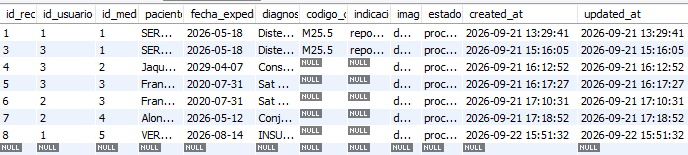
\includegraphics[width=1\textwidth]{Imagenes/tabla_recetas.png}
\caption{Registro exitoso en la tabla principal de recetas, evidenciando la generación de la llave primaria y la inserción de la información general.}
\label{fig:mysql_recetas}
\end{figure}

El punto más importante de la evaluación fue en cómo se manejó la estructura de los medicamentos. Tal como se evidencia en la Figura \ref{fig:mysql_medicamentos}, el servidor pudo recorrer el JSON e ingresar varias filas individuales en la tabla de medicamentos. También el sistema gestionó correctamente los campos con datos vacíos (aceptando la falta de información como la dosis) y conectó la clave foránea correspondiente. Esto asegura que ningún medicamento quede sin referencia, permitiendo generar un historial clínico robusto.

\begin{figure}[H]
\centering
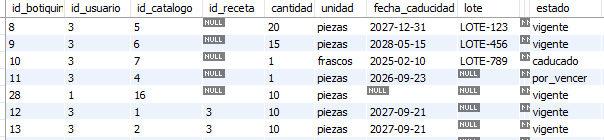
\includegraphics[width=1\textwidth]{Imagenes/tabla_medicamentos.png}
\caption{Inserción múltiple en la tabla de medicamentos. Se observa la relación mediante el id de la receta médica con un usuario.}
\label{fig:mysql_medicamentos}
\end{figure}

Es común que el modelo LLM pueda tener dificultades para identificar datos específicos si el documento físico original es ilegible o si el médico omite imprimir su cédula profesional. En lugar de generar una excepción SQL por violar las restricciones de campos obligatorios, el sistema implementa una lógica de contingencia. Como se observa en la Figura \ref{fig:mysql_medicos_contingencia}, el servidor detecta la ausencia de datos e inserta automáticamente un perfil genérico (\char`\"{}Médico Desconocido\char`\"{} y \char`\"{}Sin Cédula\char`\"{}). Esta arquitectura tolerante a fallos garantiza que el paciente siempre pueda guardar su historial de medicamentos de forma exitosa.

\begin{figure}[H]
\centering
\includegraphics[width=1\textwidth]{Imagenes/tabla_medicos_contingencia.png}
\caption{Tabla relacional de médicos ilustrando el mecanismo de contingencia. Se aprecia la inserción del perfil genérico conviviendo con perfiles de médicos reales extraídos exitosamente.}
\label{fig:mysql_medicos_contingencia}
\end{figure}

\subsubsection{Módulo de Control de Datos (CD) y Organización de Endpoints RESTful}
La primera prueba de las peticiones RESTful consistió en validar el inicio de sesión. Se configuró una petición POST hacia la ruta pública \texttt{/api/auth/google}, enviando en el cuerpo del mensaje un token simulado de Google en formato JSON. El servidor procesó la solicitud exitosamente en 358 ms, devolviendo un código 200 OK y emitiendo el JSON Web Token (JWT) que el cliente utilizará para autorizar sus futuras transacciones. La Figura \ref{fig:post_auth_google} muestra la configuración de la petición y la confirmación de la autenticación.

\begin{figure}[H]
\centering
\includegraphics[width=1\textwidth]{Imagenes/post_auth_google.png}
\caption{Configuración de la petición HTTP POST hacia la ruta de autenticación y respuesta del servidor confirmando el inicio de sesión con el código 200 OK y el JWT generado.}
\label{fig:post_auth_google}
\end{figure}

Una vez obtenido el JWT y colocado en las cabeceras de autorización, se probaron las operaciones protegidas. En la Figura \ref{fig:post_botiquin} se detalla la petición para el registro de un nuevo fármaco, donde se envió un POST a la ruta \texttt{/api/botiquin}. El \emph{middleware} validó correctamente los formatos y el servidor confirmó la inserción en 17 ms, devolviendo el código 201 Created junto con el identificador único generado por la base de datos.

\begin{figure}[H]
\centering
\includegraphics[width=1\textwidth]{Imagenes/post_botiquin.png}
\caption{Petición POST dirigida al inventario con los datos estructurales del nuevo fármaco y la respuesta de creación exitosa devolviendo el código 201 Created.}
\label{fig:post_botiquin}
\end{figure}

Posteriormente, se verificó el método de lectura mediante una petición GET a la misma ruta para recuperar el inventario. El sistema cruzó la información de manera exitosa en apenas 8 ms, recuperando un arreglo JSON exclusivamente con los medicamentos pertenecientes al usuario autenticado. La estructura de esta consulta y su exitosa respuesta se aprecian en la Figura \ref{fig:get_botiquin}.

\begin{figure}[H]
\centering
\includegraphics[width=1\textwidth]{Imagenes/get_botiquin.png}
\caption{Petición GET para la consulta general y respuesta del servidor retornando el listado del inventario médico estructurado en formato JSON.}
\label{fig:get_botiquin}
\end{figure}

Finalmente, se comprobaron las rutas de alteración de datos. Se ejecutó una petición PUT hacia \texttt{/api/botiquin/1} modificando la cantidad disponible en el inventario. El servidor procesó el cambio validando la propiedad del registro y devolvió el código 200 OK en 19 ms. De igual forma, se validó el borrado de información mediante una petición DELETE apuntando al mismo identificador, confirmando la operación con un código 200 OK en 12 ms y garantizando la correcta limpieza del historial, tal como se documenta en las pruebas presentadas en la Figura \ref{fig:put_delete_botiquin}.

\begin{figure}[H]
\centering
\includegraphics[width=1\textwidth]{Imagenes/put_delete_botiquin.png}
\caption{Confirmación de la actualización exitosa del medicamento mediante PUT y eliminación segura del registro en la base de datos a través del método DELETE.}
\label{fig:put_delete_botiquin}
\end{figure}

Todas las rutas programadas operaron de acuerdo con los requerimientos del sistema. En la Tabla \ref{tab:tiempos_api} se presenta una matriz resumen con los tiempos de respuesta obtenidos durante las simulaciones, demostrando que todas las transacciones se ejecutaron por debajo del límite de latencia aceptable (2 segundos).

\begin{table}[H]
\centering
\caption{Resultados y tiempos de ejecución de las pruebas de integración sobre la API REST.}
\label{tab:tiempos_api}
\begin{tabular}{|l|l|l|l|p{5cm}|}
\hline
\textbf{Endpoint} & \textbf{Método} & \textbf{Código HTTP} & \textbf{Tiempo} & \textbf{Resultado} \\ \hline
/api/auth/google & POST & 200 OK & 358 ms & Exitosa. Retorna JWT de sesión. \\ \hline
/api/botiquin & POST & 201 Created & 17 ms & Exitosa. Inserta y devuelve ID único. \\ \hline
/api/botiquin & GET & 200 OK & 8 ms & Exitosa. Retorna arreglo con el inventario. \\ \hline
/api/botiquin/:id & PUT & 200 OK & 19 ms & Exitosa. Actualiza datos del medicamento. \\ \hline
/api/botiquin/:id & DELETE & 200 OK & 12 ms & Exitosa. Elimina registro de la BD. \\ \hline
\end{tabular}
\end{table}


\subsection{Capa de Procesamiento y Lógica}

\subsubsection{Módulo LLM e Inteligencia Artificial Multimodal}
Para evaluar la capacidad del modelo LLM multimodal en la transcripción de recetas médicas, se llevaron a cabo peticiones al \emph{endpoint} del servidor enviando recetas reales con distintos grados de complejidad tipográfica. La operación del módulo inicia recibiendo la fotografía transformada en una cadena Base64 dentro del objeto JSON de la petición. Esta estructura, documentada en la Figura \ref{fig:payload_base64}, demuestra cómo el servidor procesa y envía el \emph{payload} directamente a la API del modelo LLM sin requerir almacenamiento local de archivos.

\begin{figure}[H]
\centering
\includegraphics[width=1\textwidth]{Imagenes/payload_base64.png}
\caption{Estructura de la petición HTTP, enviando la imagen de la receta médica codificada en formato Base64 hacia el controlador del servidor.}
\label{fig:payload_base64}
\end{figure}

Se sometió al sistema a tres escenarios de reconocimiento óptico (OCR) e interpretación:

\textbf{1. Receta con escritura semi-estructurada:} Al procesar el primer documento médico, el modelo demostró una alta precisión aislando los tres medicamentos recetados, detectando correctamente las concentraciones y las frecuencias. Sin embargo, el modelo LLM presentó una alucinación menor al transcribir la fecha de expedición, interpretando el año \char`\"{}26\char`\"{} escrito a mano como \char`\"{}24\char`\"{}, como se observa a detalle en la transcripción de la Figura \ref{fig:receta1_json}.

\begin{figure}[H]
\centering
\includegraphics[width=1\textwidth]{Imagenes/receta1_json.png}
\caption{Fotografía original de la primera receta médica evaluada y resultado JSON evidenciando la extracción exitosa de los fármacos y la variación en la lectura de la fecha.}
\label{fig:receta1_json}
\end{figure}

\textbf{2. Receta impresa con indicaciones de contexto:} En el segundo escenario, que consistía principalmente en texto impreso, el rendimiento del algoritmo fue excelente. El modelo no solo estructuró los medicamentos de manera ideal, sino que el diseño de las instrucciones (el \emph{prompt}) logró capturar indicaciones médicas complicadas (como las fechas de reposo y los datos de infección en el codo) que se encontraban fuera del formato tabular. La Figura \ref{fig:receta2_json} documenta esta extracción perfecta.

\begin{figure}[H]
\centering
\includegraphics[width=1\textwidth]{Imagenes/receta2_json.png}
\caption{Fotografía original de la segunda receta médica evaluada y resultado JSON, demostrando el reconocimiento perfecto del texto impreso y la captura del contexto clínico adicional.}
\label{fig:receta2_json}
\end{figure}

\textbf{3. Receta con caligrafía cursiva compleja:} El tercer escenario representó un gran desafío. Al procesar texto cursivo de difícil legibilidad, el modelo LLM cometió errores significativos. Omitió caracteres en el nombre del paciente, interpretó mal la fecha y falló en la interpretación de la posología del medicamento simplificando erróneamente \char`\"{}cada 12 hrs por 3 a 5 días\char`\"{} a \char`\"{}3 al día\char`\"{}, lo cual se hace evidente en los fallos mostrados en la Figura \ref{fig:receta3_json}.

\begin{figure}[H]
\centering
\includegraphics[width=1\textwidth]{Imagenes/receta3_json.png}
\caption{Fotografía de la tercera receta médica presentando alta dificultad caligráfica y su resultado JSON evidenciando fallos de interpretación generados por la complejidad de la escritura en las instrucciones de uso.}
\label{fig:receta3_json}
\end{figure}

Las variaciones observadas en la tercera prueba representan un riesgo clínico potencial. Para mitigar este margen de error inherente al modelo LLM, el diseño de la arquitectura general dicta que este objeto JSON devuelto por el \emph{backend} NUNCA SE GUARDARÁ AUTOMÁTICAMENTE EN LA BASE DE DATOS. Por el contrario, los datos extraídos serán enviados a la aplicación \emph{frontend}, obligando a la persona usuaria a realizar una validación visual final \emph{(Human-in-the-loop)}.


\subsubsection{Módulo de Ubicación de Farmacias}
Al inicializar el módulo, el sistema logra obtener las coordenadas (longitud, latitud) del dispositivo y envía estos datos al \emph{backend}. Tal como se muestra en la Figura \ref{fig:mapa_dividido}, la interfaz procesa el arreglo JSON que genera el servidor y renderiza dos vistas al mismo tiempo. Por un lado, se muestran los establecimientos ordenándolos desde el más cercano al más lejano. Al mismo tiempo, se despliega el mapa sin ruido, confirmando la posición de la persona usuaria y mostrando los marcadores alrededor en el radio de búsqueda.

\begin{figure}[H]
\centering
\includegraphics[width=1\textwidth]{Imagenes/mapa_dividido.png}
\caption{Interfaz dividida mostrando el listado de farmacias ordenado por distancia y el renderizado del mapa con los marcadores personalizados sobre la ubicación real.}
\label{fig:mapa_dividido}
\end{figure}

El componente emergente reacciona mostrando la distancia exacta calculada por el motor y el horario del establecimiento. En la Figura \ref{fig:mapa_marcador} se comprueba el comportamiento del componente interactivo y el correcto funcionamiento del botón \char`\"{}Cómo llegar\char`\"{}, el cual enruta exitosamente las coordenadas de destino actuando como puente hacia servicios de navegación externos.

\begin{figure}[H]
\centering
\includegraphics[width=1\textwidth]{Imagenes/mapa_marcador.png}
\caption{Despliegue del módulo interactivo sobre un marcador específico, revelando información del establecimiento y el botón de redirección hacia el servicio de navegación.}
\label{fig:mapa_marcador}
\end{figure}

En la búsqueda manual, la incorporación del módulo de Geocodificación y la aplicación del patrón \emph{Debounce} mostraron un rendimiento excelente. Al comenzar a teclear una dirección (por ejemplo \char`\"{}Uam azc\char`\"{}), el sistema demuestra la efectividad de la protección. En lugar de saturar el servidor con una petición por cada letra, el sistema aguarda un límite de tiempo y despliega un menú flotante con los resultados exactos devueltos por Geoapify (Figura \ref{fig:busqueda_debounce}).

\begin{figure}[H]
\centering
\includegraphics[width=1\textwidth]{Imagenes/busqueda_debounce.png}
\caption{Estado inicial del componente de búsqueda y menú flotante de autocompletado desplegando sugerencias precisas en respuesta a la entrada de texto del usuario.}
\label{fig:busqueda_debounce}
\end{figure}

Al hacer clic sobre una sugerencia, este cambio de estado dispara automáticamente una nueva petición, actualizando el panel lateral y el mapa con las farmacias más cercanas a la nueva ubicación seleccionada, lo cual se ilustra claramente en la Figura \ref{fig:mapa_actualizado}.

\begin{figure}[H]
\centering
\includegraphics[width=1\textwidth]{Imagenes/mapa_actualizado.png}
\caption{Panel lateral reflejando la actualización del arreglo de datos y mapa actualizado a la dirección buscada manualmente con etiquetas dinámicas sobre los marcadores geográficos.}
\label{fig:mapa_actualizado}
\end{figure}


\subsubsection{Módulo de Consulta de Precios Comerciales}
El módulo presenta una interfaz intuitiva y una conexión en tiempo real con el motor de Google Shopping (vía SerpApi). La persona usuaria puede ingresar el nombre del medicamento para comparar precios. Por ejemplo, al ingresar \char`\"{}ibuprofeno\char`\"{}, el sistema clasificó de forma automática los productos, ordenándolos de menor a mayor precio. Como se puede observar en la Figura \ref{fig:consulta_precios}, el sistema logró extraer y procesar toda la información de manera limpia y clara.

\begin{figure}[H]
\centering
\includegraphics[width=1\textwidth]{Imagenes/consulta_precios.png}
\caption{Interfaz principal de búsqueda interactiva y organización de las ofertas comerciales, mostrando fotografías del producto, tienda vendedora y la etiqueta destacada para la opción más económica.}
\label{fig:consulta_precios}
\end{figure}

El sistema logró extraer la fotografía real del medicamento, su nombre comercial exacto, el precio y la tienda que lo oferta. Además, el sistema evalúa los costos e inserta una etiqueta de MEJOR OPCIÓN en el primer resultado. Cada oferta se acompaña de un botón \char`\"{}Más detalles\char`\"{}, guiando a la persona a la página de compra adecuada.


\subsubsection{Módulo de Accesibilidad: Voz-Texto y Texto-Voz}
El primer paso de la interacción ocurre cuando el usuario decide utilizar la herramienta de dictado. Para garantizar la privacidad, el navegador intercepta la petición y solicita el permiso para acceder al hardware del micrófono. Una vez concedido, la interfaz cambia para indicar que se encuentra en modo de escucha, mostrando la transcripción del audio a texto en tiempo real, proceso ilustrado en la Figura \ref{fig:permisos_microfono}.

\begin{figure}[H]
\centering
\includegraphics[width=1\textwidth]{Imagenes/permisos_microfono.png}
\caption{Solicitud de permisos de hardware por parte del navegador y activación del estado de escucha en la interfaz.}
\label{fig:permisos_microfono}
\end{figure}

Se verificó la capacidad del sistema para interpretar los síntomas bajo diferentes condiciones de ruido. En condiciones normales, el motor capturó el 100\% de la frase con la ortografía correcta (\char`\"{}Me duele la cabeza, tengo náuseas y fiebre de 38 grados\char`\"{}). Ante ruido moderado, la transcripción presentó un ligero incremento en la latencia, logrando aislar la voz principal. Con ruido agresivo en ambiente de calle, logró acertar en un 90\% la descripción, demostrando ser altamente funcional. En la Figura \ref{fig:transcripcion_voz} se aprecia cómo, a medida que el paciente narra sus síntomas de forma natural, el texto se transcribe progresivamente.

\begin{figure}[H]
\centering
\includegraphics[width=1\textwidth]{Imagenes/transcripcion_voz.png}
\caption{Transcripción automática en tiempo real de los síntomas dictados por la persona usuaria con un diseño limpio que evita distracciones.}
\label{fig:transcripcion_voz}
\end{figure}

Adicionalmente, se comprobaron escenarios tolerantes a fallos donde la persona usuaria bloquea el acceso al micrófono. El sistema no presentó excepciones no controladas de JavaScript. El flujo alterno funcionó permitiendo utilizar el área de texto como un formulario de ingreso manual sin bloquear la interfaz.

Finalmente, el desarrollo de la síntesis de voz (\emph{Text-to-Speech}) permitió generar un guion de manera coherente. La velocidad de lectura preconfigurada en 0.9 resultó óptima para evitar una síntesis acelerada, garantizando que adultos mayores procesen la información de manera pausada y natural.


\subsubsection{Módulo de Procesamiento de Lenguaje Natural (CIE-10 y NLP)}
Se ejecutó el módulo procesando frases informales con un alto nivel de ruido gramatical, como: \char`\"{}¡Ay! Me duele muchísimo la cabeza, y tengo un fuerte dolor en la panza\char`\"{}. El motor NLP aplicó la normalización, descartando todo el ruido y extrayendo de manera limpia los conceptos anatómicos clave registrados en el diccionario: ['cabeza', 'panza']. Como se documenta en la Figura \ref{fig:tokenizacion_consola}, el algoritmo reconoció y descartó todo el ruido exitosamente.

\begin{figure}[H]
\centering
\includegraphics[width=1\textwidth]{Imagenes/tokenizacion_consola.png}
\caption{Resultados en consola de la tokenización y normalización de texto. El motor filtra exitosamente las palabras vacías y extrae únicamente las entidades de interés.}
\label{fig:tokenizacion_consola}
\end{figure}

A partir de las entidades aisladas, el sistema asoció la palabra \char`\"{}cabeza\char`\"{} con el código R51 y \char`\"{}panza\char`\"{} con el código R10, generando un arreglo estructurado en JSON con los diagnósticos oficiales (\char`\"{}Cefalea\char`\"{} y \char`\"{}Dolor abdominal y pélvico\char`\"{}). La Figura \ref{fig:mapeo_nlp} ilustra cómo el algoritmo asoció matemáticamente estas palabras a la clasificación estandarizada.

\begin{figure}[H]
\centering
\includegraphics[width=1\textwidth]{Imagenes/mapeo_nlp.png}
\caption{Asociación de las entidades extraídas. El sistema vincula las palabras con sus códigos CIE-10 y retorna el arreglo estructurado con los diagnósticos oficiales correspondientes.}
\label{fig:mapeo_nlp}
\end{figure}

Se comprobó la protección de seguridad del algoritmo. Al enviar una petición extensa sin el \emph{token} de autorización, el servidor emitió un código 403 Forbidden interceptando la solicitud, demostrando que la carga del NLP funciona en un entorno seguro (Figura \ref{fig:nlp_forbidden}).

\begin{figure}[H]
\centering
\includegraphics[width=1\textwidth]{Imagenes/nlp_forbidden.png}
\caption{Bloqueo de la petición por parte del servidor, protegiendo el recurso analítico ante la ausencia de un token válido.}
\label{fig:nlp_forbidden}
\end{figure}

Con un JWT válido, el algoritmo asigna probabilidades matemáticas a múltiples afecciones y prioriza los resultados. Al dictar \char`\"{}Ayer empecé con mucha tos y hoy amanecí con calentura. Además, me duele horrible la cabeza...\char`\"{}, el sistema filtró exitosamente \char`\"{}Náusea (R11.0)\char`\"{}, \char`\"{}Cefalea (R51)\char`\"{} y \char`\"{}Tos (R05)\char`\"{}, devolviéndolos ordenados jerárquicamente por probabilidad y descartando dinámicamente diagnósticos de menor peso. La Figura \ref{fig:nlp_probabilidad} muestra cómo el algoritmo calcula este puntaje con base en las incidencias.

\begin{figure}[H]
\centering
\includegraphics[width=1\textwidth]{Imagenes/nlp_probabilidad.png}
\caption{Respuesta exitosa del servidor (200 OK) mostrando el Top 3 de diagnósticos, ordenados matemáticamente por su probabilidad y jerarquizados mediante el número de coincidencias.}
\label{fig:nlp_probabilidad}
\end{figure}


\subsection{Capa de Visualización}

\subsubsection{Módulo de Captura de Fotografía}
La prueba de integración de la interfaz inicia en la pantalla principal. Al seleccionar el documento, el sistema local transforma la imagen a Base64 y dispara la petición HTTP hacia el \emph{backend}. La Figura \ref{fig:escaner_principal} muestra la pantalla principal que centra la atención del usuario hacia la carga del documento.

\begin{figure}[H]
\centering
\includegraphics[width=1\textwidth]{Imagenes/escaner_principal.png}
\caption{Interfaz principal para subir imagen de receta, lista para inicializar la conversión de la imagen a Base64.}
\label{fig:escaner_principal}
\end{figure}

Para evitar el bloqueo del hilo principal durante la lectura de archivos pesados, la función \texttt{convertirABase64} encapsula el proceso en una Promesa. El algoritmo instancia \texttt{FileReader}, lee los bytes y limpia los metadatos iniciales mediante una expresión regular como se expone en la Figura \ref{fig:codigo_base64}.

\begin{figure}[H]
\centering
\includegraphics[width=1\textwidth]{Imagenes/codigo_base64.png}
\caption{Función que convierte un archivo local a un \emph{string} Base64 purificado para ser enviado al \emph{backend}.}
\label{fig:codigo_base64}
\end{figure}

Inmediatamente después de disparar la petición, el sistema despliega un estado de carga a pantalla completa. La Figura \ref{fig:pantalla_carga} ejemplifica este comportamiento que demostró ser efectivo para bloquear la interacción del usuario y proteger el flujo evitando peticiones duplicadas.

\begin{figure}[H]
\centering
\includegraphics[width=1\textwidth]{Imagenes/pantalla_carga.png}
\caption{Pantalla de carga inmersiva, bloqueando exitosamente la interfaz de usuario durante la espera de la respuesta del backend.}
\label{fig:pantalla_carga}
\end{figure}


\subsubsection{Interfaz Web y Responsividad}
Al recibir la respuesta exitosa del servidor, la interfaz aplica el patrón \emph{Human-in-the-loop} desplegando el modal de validación de datos. Se comprobó la capa de retroalimentación visual: si se procesa una receta sin cédula profesional, el \emph{frontend} detona una alerta roja advirtiendo sobre la invalidez oficial del documento. Como se observa en la Figura \ref{fig:alerta_seguridad}, este comportamiento protege la fidelidad del expediente.

\begin{figure}[H]
\centering
\includegraphics[width=1\textwidth]{Imagenes/alerta_seguridad.png}
\caption{Modal de revisión de datos (Human-in-the-loop), mostrando la respuesta exitosa de la información general y la activación automática de la alerta de seguridad clínica.}
\label{fig:alerta_seguridad}
\end{figure}

El listado de medicamentos devuelto por el servidor se presenta de manera interactiva. Cada campo (dosis, formato, instrucciones) es editable, permitiendo a la persona usuaria corregir cualquier mala transcripción del LLM antes de guardar la información final. La Figura \ref{fig:listado_editable} muestra el listado de medicamentos devuelto por el servidor completamente manipulable.

\begin{figure}[H]
\centering
\includegraphics[width=1\textwidth]{Imagenes/listado_editable.png}
\caption{Listado de medicamentos que devolvió el servidor. Los campos editables garantizan la supervisión humana sobre la extracción automatizada.}
\label{fig:listado_editable}
\end{figure}

En la sección de resultados del \emph{Fuzzy Matching} y NLP, la interfaz generó los tres contenedores esperados. En la cabecera, se probó exitosamente la visualización de avisos legales recordando que el software no sustituye el criterio médico. También, al existir coincidencia (\char`\"{}Cefalea\char`\"{}), la interfaz muestra correctamente que hay \char`\"{}Tylenol\char`\"{} con \char`\"{}24 unidades\char`\"{} en el inventario actual. En la Figura \ref{fig:resultados_fuzzy} se refleja el éxito del algoritmo de Fuzzy Matching.

\begin{figure}[H]
\centering
\includegraphics[width=1\textwidth]{Imagenes/resultados_fuzzy.png}
\caption{Texto final validado por el usuario y visualización de los padecimientos detectados, extracción de palabras clave y su vinculación con el inventario de recetas previas.}
\label{fig:resultados_fuzzy}
\end{figure}

Para comprobar la usabilidad general del \emph{frontend}, se verificó que los módulos se adaptaran a pantallas pequeñas (Mobile-First) simulando un \emph{viewport} vertical de 360x800 píxeles. Los elementos de la interfaz se redistribuyeron de forma ordenada. Los botones principales mantuvieron un tamaño adecuado previniendo pulsaciones accidentales, y la tabla comparativa de precios ajustó su contenido sin distorsionar el diseño general.

Por último, en cuanto a prevención de errores, se simularon desconexiones repentinas y caídas de servidores. La aplicación abortó peticiones de red a tiempo y notificó el problema mediante tarjetas visuales integradas (sin usar ventanas emergentes obstructivas), demostrando una solidez excepcional en el manejo de excepciones para el usuario final.


\clearpage

\section{Análisis y discusión de resultados}

\clearpage

\section{Conclusiones}

\clearpage

\referencias %Esta línea se debe mantener

\clearpage


\section{Anexos}

\subsection*{Anexo A: llmAdapter.js}
\begin{lstlisting}[language=JavaScript, breaklines=true]
/**
 * server/src/services/llmAdapter.js
 */
const { GoogleGenerativeAI } = require('@google/generative-ai');
const Groq = require('groq-sdk');
const config = require('../config/env');

const procesarConGroq = async (prompt, base64Image) => {
  const groq = new Groq({ apiKey: config.ai.groqApiKey });
  const response = await groq.chat.completions.create({
    model: 'qwen-2.5-vl-72b-instruct',
    messages: [
      {
        role: 'user',
        content: [
          { type: 'text', text: prompt },
          {
            type: 'image_url',
            image_url: { url: `data:image/jpeg;base64,${base64Image}` },
          },
        ],
      },
    ],
    response_format: { type: 'json_object' },
  });
  return response.choices[0]?.message?.content;
};

const procesarVisionLLM = async (prompt, cleanBase64) => {
  const provider = process.env.AI_PROVIDER || 'gemini';
  if (provider === 'groq') {
    return await procesarConGroq(prompt, cleanBase64);
  }
  // Fallback por defecto a Gemini
  const imagePart = { inlineData: { data: cleanBase64, mimeType: 'image/jpeg' } };
  return await require('./visionService').procesarConGemini(prompt, imagePart);
};

module.exports = { procesarVisionLLM };

\end{lstlisting}

\subsection*{Anexo B: jsonParser.js}
\begin{lstlisting}[language=JavaScript, breaklines=true]
/**
 * server/src/utils/jsonParser.js
 * Extrae y parsea objetos JSON devueltos por LLMs de manera tolerante a fallos.
 */
const extraerJsonSeguro = (texto) => {
  if (!texto || typeof texto !== 'string') {
    throw new Error('La respuesta del modelo está vacía o es inválida.');
  }

  try {
    const clean = texto.replace(/```json/gi, '').replace(/```/g, '').trim();
    return JSON.parse(clean);
  } catch (err) {
    const jsonMatch = texto.match(/\{[\s\S]*\}/);
    if (jsonMatch) {
      try {
        return JSON.parse(jsonMatch[0]);
      } catch (innerErr) {
        throw new Error(`Estructura JSON malformada en la salida del modelo: ${innerErr.message}`);
      }
    }
    throw new Error('No se encontró una estructura JSON reconocible en la respuesta del LLM.');
  }
};

module.exports = { extraerJsonSeguro };

\end{lstlisting}

\subsection*{Anexo C: useFarmacias.js}
\begin{lstlisting}[language=JavaScript, breaklines=true]
import { useState, useEffect } from 'react';
import api from '../services/api';
import toast from 'react-hot-toast';
import SpeechRecognition, { useSpeechRecognition } from 'react-speech-recognition';

export const useFarmacias = () => {
  const [seccionActiva, setSeccionActiva] = useState('precios');
  
  // Estado del Mapa
  const [coords, setCoords] = useState(() => {
    const savedCoords = localStorage.getItem('bdi_last_location');
    if (savedCoords) {
      try {
        return JSON.parse(savedCoords);
      } catch (e) {
        // Ignorar error de parseo
      }
    }
    return null;
  });

  useEffect(() => {
    localStorage.setItem('bdi_last_location', JSON.stringify(coords));
  }, [coords]);
  const [farmacias, setFarmacias] = useState([]);
  const [cargandoFarmacias, setCargandoFarmacias] = useState(false);

  // Estado de Precios
  const [terminoPrecios, setTerminoPrecios] = useState('');
  const [precios, setPrecios] = useState([]);
  const [buscandoPrecios, setBuscandoPrecios] = useState(false);
  const [historialCotizaciones, setHistorialCotizaciones] = useState([]);
  const [ordenPrecio, setOrdenPrecio] = useState('popularidad');

  const { transcript, listening, resetTranscript, browserSupportsSpeechRecognition } = useSpeechRecognition();

  useEffect(() => {
    if (seccionActiva === 'precios' && listening && transcript) {
      setTerminoPrecios(transcript);
    }
  }, [transcript, listening, seccionActiva]);

  useEffect(() => {
    if (seccionActiva === 'precios' && !listening && transcript && terminoPrecios === transcript) {
      handleCotizarPrecios(transcript);
    }
    // eslint-disable-next-line react-hooks/exhaustive-deps
  }, [listening, seccionActiva]);

  const toggleVoz = () => {
    if (!browserSupportsSpeechRecognition) {
      toast.error('Tu navegador no soporta reconocimiento de voz.');
      return;
    }
    if (listening) {
      SpeechRecognition.stopListening();
    } else {
      resetTranscript();
      SpeechRecognition.startListening({ continuous: false, language: 'es-MX' });
    }
  };

  useEffect(() => {
    const cargarHistorial = async () => {
      try {
        const res = await api.get('/farmacias/historial');
        if (res.data) setHistorialCotizaciones(res.data);
      } catch (e) {
        // Silencioso
      }
    };
    cargarHistorial();
  }, []);

  const cargarFarmacias = async (lat, lng) => {
    setCargandoFarmacias(true);
    try {
      const res = await api.post('/farmacias/cercanas', { lat, lng });
      if (res.data) setFarmacias(res.data);
    } catch (err) {
      toast.error('Error al localizar farmacias cercanas.');
    } finally {
      setCargandoFarmacias(false);
    }
  };

  const handleUsarGPS = () => {
    if (!navigator.geolocation) {
      toast.error('Geolocalización no soportada por el navegador.');
      const fallback = { lat: 19.4326, lng: -99.1332, nombre: 'Ciudad de México (Centro)' };
      setCoords(fallback);
      cargarFarmacias(fallback.lat, fallback.lng);
      return;
    }

    const toastId = toast.loading('Obteniendo ubicación GPS precisa...');

    const obtenerPosicion = (opts) =>
      new Promise((resolve, reject) => {
        navigator.geolocation.getCurrentPosition(resolve, reject, opts);
      });

    (async () => {
      let pos;
      try {
        pos = await obtenerPosicion({ enableHighAccuracy: true, timeout: 9000, maximumAge: 0 });
      } catch (errHigh) {
        console.warn('GPS alta precisión falló o demoró, intentando precisión estándar...', errHigh);
        try {
          pos = await obtenerPosicion({ enableHighAccuracy: false, timeout: 10000, maximumAge: 60000 });
        } catch (errFallback) {
          throw errFallback;
        }
      }

      const lat = pos.coords.latitude;
      const lng = pos.coords.longitude;
      const accuracy = pos.coords.accuracy;

      let direccionLegible = `Ubicación GPS (${lat.toFixed(4)}, ${lng.toFixed(4)})`;
      try {
        const res = await api.get(`/farmacias/reversa?lat=${lat}&lng=${lng}`);
        if (res.data?.direccionFormateada) {
          direccionLegible = res.data.direccionFormateada;
        }
      } catch (e) {
        console.warn('Error en reverse geocoding:', e);
      }

      const nuevasCoords = {
        lat,
        lng,
        nombre: direccionLegible,
      };

      setCoords(nuevasCoords);
      cargarFarmacias(lat, lng);

      if (accuracy && accuracy > 800) {
        toast.success(
          `GPS aproximado (~${Math.round(accuracy)}m). Puedes afinar haciendo clic en el mapa.`,
          { id: toastId, duration: 6000 }
        );
      } else {
        toast.success('Ubicación GPS detectada con éxito.', { id: toastId });
      }
    })().catch((error) => {
      console.error('Error al obtener GPS:', error);
      let msg = 'No se pudo obtener la ubicación GPS.';
      if (error?.code === 1) {
        msg = 'Permiso de ubicación denegado en tu navegador. Puedes escribir tu dirección en el buscador.';
      } else if (error?.code === 2) {
        msg = 'Señal de ubicación no disponible. Puedes buscar tu colonia o alcaldía en la barra.';
      } else if (error?.code === 3) {
        msg = 'Tiempo de espera de GPS agotado. Escribe tu calle o colonia para localizar farmacias.';
      }
      toast.error(msg, { id: toastId, duration: 6000 });
      
      // Fallback
      const fallback = { lat: 19.4326, lng: -99.1332, nombre: 'Ciudad de México (Centro)' };
      setCoords(fallback);
      cargarFarmacias(fallback.lat, fallback.lng);
    });
  };

  useEffect(() => {
    if (coords) {
      cargarFarmacias(coords.lat, coords.lng);
    } else {
      handleUsarGPS();
    }
    // eslint-disable-next-line react-hooks/exhaustive-deps
  }, []);



  const handleMoverUbicacion = async (lat, lng) => {
    let direccionLegible = `Ubicación ajustada (${lat.toFixed(4)}, ${lng.toFixed(4)})`;
    try {
      const res = await api.get(`/farmacias/reversa?lat=${lat}&lng=${lng}`);
      if (res.data?.direccionFormateada) {
        direccionLegible = res.data.direccionFormateada;
      }
    } catch (e) {
      console.warn('Error en reverse geocoding al mover:', e);
    }

    const nuevasCoords = { lat, lng, nombre: direccionLegible };
    setCoords(nuevasCoords);
    cargarFarmacias(lat, lng);
    toast.success('Ubicación actualizada en el mapa.');
  };

  const handleSeleccionarUbicacion = (lat, lng, direccion) => {
    const nuevasCoords = { lat, lng, nombre: direccion };
    setCoords(nuevasCoords);
    cargarFarmacias(lat, lng);
    toast.success(`Ubicación establecida: ${direccion || 'Coordenadas seleccionadas'}`);
  };

  const handleCotizarPrecios = async (medicamentoAconsultar) => {
    const med = medicamentoAconsultar || terminoPrecios;
    if (!med || !med.trim()) {
      toast.error('Escribe el nombre de un medicamento para cotizar.');
      return;
    }

    setBuscandoPrecios(true);
    setPrecios([]);
    try {
      const res = await api.post('/farmacias/buscar', { medicamento: med.trim() });
      if (res.data) {
        setPrecios(res.data);
        toast.success(`Se encontraron ${res.data.length} ofertas para ${med}.`);
      }
    } catch (err) {
      toast.error(err.message || 'Error al cotizar precios.');
    } finally {
      setBuscandoPrecios(false);
    }
  };

  return {
    seccionActiva,
    setSeccionActiva,
    coords,
    farmacias,
    cargandoFarmacias,
    terminoPrecios,
    setTerminoPrecios,
    precios,
    buscandoPrecios,
    historialCotizaciones,
    ordenPrecio,
    setOrdenPrecio,
    listening,
    toggleVoz,
    handleUsarGPS,
    handleMoverUbicacion,
    handleSeleccionarUbicacion,
    handleCotizarPrecios
  };
};

\end{lstlisting}

\subsection*{Anexo D: serpapiService.js}
\begin{lstlisting}[language=JavaScript, breaklines=true]
const { getJson } = require('serpapi');
const config = require('../config/env');

/**
 * Consulta ofertas comerciales de medicamentos en Google Shopping México vía SerpApi.
 * 
 * @param {string} medicamentoNombre - Término de búsqueda (ej. "Paracetamol 500mg")
 * @returns {Promise<Array<Object>>} Lista de ofertas normalizadas
 */
const buscarPreciosMedicamento = async (medicamentoNombre) => {
  const apiKey = config.serpapi.apiKey;

  if (!apiKey || apiKey === 'YOUR_SERPAPI_KEY_HERE') {
    console.warn('[SerpApi] Clave API no configurada, devolviendo datos simulados locales.');
    return [
      {
        title: `${medicamentoNombre} 20 tabletas`,
        price: '$42.50',
        store: 'Farmacias del Ahorro',
        link: 'https://www.fahorro.com',
        thumbnail: 'https://images.unsplash.com/photo-1584308666744-24d5c474f2ae?w=150',
      },
      {
        title: `${medicamentoNombre} Genérico 500mg`,
        price: '$28.00',
        store: 'Farmacias Similares',
        link: 'https://farmaciasdesimilares.com',
        thumbnail: 'https://images.unsplash.com/photo-1584308666744-24d5c474f2ae?w=150',
      },
      {
        title: `${medicamentoNombre} Patente Caja c/24`,
        price: '$98.00',
        store: 'Farmacia San Pablo',
        link: 'https://www.farmaciasanpablo.com.mx',
        thumbnail: 'https://images.unsplash.com/photo-1584308666744-24d5c474f2ae?w=150',
      },
    ];
  }

  try {
    const axios = require('axios');
    const { data } = await axios.get('https://serpapi.com/search.json', {
      params: {
        api_key: apiKey,
        engine: 'google_shopping',
        q: `${medicamentoNombre} medicamento farmacia`,
        gl: 'mx',
        hl: 'es',
        google_domain: 'google.com.mx',
        num: 15,
      },
      timeout: 15000 // 15 segundos máximo
    });

    if (!data) {
      throw new Error('Respuesta vacía de SerpApi');
    }
    if (data.error) {
      if (data.error.includes("Google hasn't returned any results")) {
        return []; // Retorna lista vacía en lugar de lanzar error
      }
      throw new Error(`Error de SerpApi: ${data.error}`);
    }

    const items = data.shopping_results || [];
    const resultados = items.map((item) => ({
      title: item.title,
      price: item.price || item.extracted_price ? `$${item.extracted_price}` : 'Consultar tienda',
      store: item.source || item.merchant?.name || 'Farmacia en línea',
      link: item.link || item.product_link || '#',
      thumbnail: item.thumbnail || null,
    }));

    return resultados;
  } catch (error) {
    if (error.response && error.response.data && error.response.data.error) {
       const apiError = error.response.data.error;
       if (apiError.includes("Google hasn't returned any results")) return [];
       throw new Error(`Error de SerpApi: ${apiError}`);
    }
    throw new Error(error.message || 'Error al conectar con SerpApi');
  }
};

/**
 * Calcula la distancia en metros entre dos coordenadas geográficas mediante la fórmula de Haversine.
 */
const calcularDistanciaMetros = (lat1, lon1, lat2, lon2) => {
  if (!lat1 || !lon1 || !lat2 || !lon2) return null;
  const R = 6371e3;
  const φ1 = (lat1 * Math.PI) / 180;
  const φ2 = (lat2 * Math.PI) / 180;
  const Δφ = ((lat2 - lat1) * Math.PI) / 180;
  const Δλ = ((lon2 - lon1) * Math.PI) / 180;

  const a =
    Math.sin(Δφ / 2) * Math.sin(Δφ / 2) +
    Math.cos(φ1) * Math.cos(φ2) * Math.sin(Δλ / 2) * Math.sin(Δλ / 2);
  const c = 2 * Math.atan2(Math.sqrt(a), Math.sqrt(1 - a));

  return Math.round(R * c);
};

/**
 * Busca farmacias físicas cercanas utilizando SerpApi (Google Maps Engine).
 * Retorna nombre, coordenadas, puntuación (rating), número de reseñas,
 * teléfono, estado abierto/cerrado y horario completo.
 * 
 * @param {number} lat - Latitud
 * @param {number} lng - Longitud
 * @returns {Promise<Array<Object>>}
 */
const buscarFarmaciasCercanas = async (lat, lng) => {
  const apiKey = config.serpapi.apiKey;
  if (!apiKey || apiKey === 'YOUR_SERPAPI_KEY_HERE') {
    return [];
  }

  try {
    const axios = require('axios');
    const { data } = await axios.get('https://serpapi.com/search.json', {
      params: {
        engine: 'google_maps',
        q: 'farmacias',
        ll: `@${lat},${lng},14z`,
        type: 'search',
        hl: 'es',
        api_key: apiKey,
      },
      timeout: 15000
    });

    if (!data || data.error) {
      if (data?.error) console.warn('[SerpApi Google Maps Warning]:', data.error);
      return [];
    }

    const items = data.local_results || [];
    const farmacias = items
      .filter((r) => r.title && r.gps_coordinates?.latitude && r.gps_coordinates?.longitude)
      .map((r) => {
        const fLat = r.gps_coordinates.latitude;
        const fLng = r.gps_coordinates.longitude;
        const dist = calcularDistanciaMetros(lat, lng, fLat, fLng);

        return {
          id: r.place_id || r.data_id || String(Math.random()),
          nombre: r.title,
          direccion: r.address || 'Dirección no especificada',
          lat: fLat,
          lng: fLng,
          rating: typeof r.rating === 'number' ? r.rating : null,
          reviews: typeof r.reviews === 'number' ? r.reviews : null,
          telefono: r.phone || null,
          abierto: r.open_state || r.hours || null,
          horario: r.open_state || r.hours || 'Consulta horario',
          distanciaMetros: dist,
          thumbnail: r.thumbnail || null,
          website: r.website || null,
        };
      });

    farmacias.sort((a, b) => (a.distanciaMetros || 0) - (b.distanciaMetros || 0));
    return farmacias;
  } catch (error) {
    console.warn('[SerpApi Google Maps Error]:', error.message);
    return [];
  }
};

module.exports = { 
  buscarPreciosMedicamento,
  buscarFarmaciasCercanas,
};

\end{lstlisting}

\subsection*{Anexo E: nlpService.js}
\begin{lstlisting}[language=JavaScript, breaklines=true]
const { NlpManager } = require('node-nlp');
const pool = require('../config/db');

// Configuración del motor NLP en español con NER forzado
const manager = new NlpManager({
  languages: ['es'],
  forceNER: true,
  nlu: { log: false },
});

let isInitialized = false;

/**
 * Carga el catálogo de diagnósticos CIE-10 desde MySQL y entrena el motor NER.
 */
const inicializarMotorNLP = async () => {
  try {
    console.log('[NLP Service] Cargando catálogo CIE-10 desde MySQL...');
    const [diagnosticos] = await pool.query('SELECT codigo_cie10, keywords FROM catalogo_cie10');

    if (!diagnosticos || diagnosticos.length === 0) {
      console.warn('[NLP Service] No se encontraron registros en catalogo_cie10. Ejecuta el seed SQL.');
      return;
    }

    diagnosticos.forEach((diag) => {
      const idEntidad = diag.codigo_cie10;
      let keywords = diag.keywords;

      if (typeof keywords === 'string') {
        try {
          keywords = JSON.parse(keywords);
        } catch (e) {
          keywords = [];
        }
      }

      if (Array.isArray(keywords) && keywords.length > 0) {
        manager.addNamedEntityText(idEntidad, idEntidad, ['es'], keywords);
      }
    });

    await manager.train();
    isInitialized = true;
    console.log(`[NLP Service] Motor NER entrenado exitosamente con ${diagnosticos.length} categorías CIE-10.`);
  } catch (error) {
    console.error('[NLP Service Error] Error al inicializar el motor NLP:', error.message);
  }
};

/**
 * Procesa una frase del usuario para identificar entidades y códigos CIE-10 correspondientes.
 * 
 * @param {string} frase - Texto o transcripción de síntomas
 * @returns {Promise<Object>} { resultadosBrutos, entidadesDetectadas }
 */
const buscarDiagnosticos = async (frase) => {
  if (!isInitialized) {
    await inicializarMotorNLP();
  }

  const analisis = await manager.process('es', frase);

  if (!analisis.entities || analisis.entities.length === 0) {
    return { resultadosBrutos: [], entidadesDetectadas: [] };
  }

  const codigosEncontrados = [...new Set(analisis.entities.map((e) => e.entity))];

  try {
    const [resultadosBrutos] = await pool.query(
      'SELECT id_diagnostico, codigo_cie10, termino_medico, capitulo, keywords FROM catalogo_cie10 WHERE codigo_cie10 IN (?)',
      [codigosEncontrados]
    );

    return {
      resultadosBrutos,
      entidadesDetectadas: analisis.entities,
    };
  } catch (error) {
    console.error('[NLP Service Error] Error al consultar diagnósticos en BD:', error.message);
    return { resultadosBrutos: [], entidadesDetectadas: [] };
  }
};

module.exports = {
  inicializarMotorNLP,
  buscarDiagnosticos,
  manager,
};

\end{lstlisting}

\subsection*{Anexo F: symptomController.js}
\begin{lstlisting}[language=JavaScript, breaklines=true]
const { buscarDiagnosticos } = require('../services/nlpService');
const { aplicarFiltroRelevancia } = require('../utils/filtroRelevancia');
const pool = require('../config/db');

/**
 * Analiza la descripción de síntomas en lenguaje natural mediante el motor NLP,
 * clasifica a CIE-10, aplica filtro de relevancia determinista (Top-3) y cruza
 * los hallazgos con el historial clínico y el stock físico del botiquín.
 */
const analizarSintomas = async (req, res, next) => {
  const { frase } = req.body;
  const idUsuario = req.usuario ? req.usuario.id_usuario : null;

  if (!frase || typeof frase !== 'string' || frase.trim().length === 0) {
    return res.status(400).json({
      exito: false,
      error: "Debes proporcionar una 'frase' válida con la descripción de los síntomas.",
    });
  }

  try {
    // 1. Extracción de entidades clínicas mediante NLP NER
    const extraccion = await buscarDiagnosticos(frase);

    if (extraccion.resultadosBrutos.length === 0) {
      return res.status(200).json({
        exito: true,
        mensaje: 'No se detectaron entidades clínicas específicas en la frase dictada.',
        resultados: [],
        historial: [],
      });
    }

    // 2. Aplicar algoritmo de relevancia (Scoring >= 50% y Top-3)
    const resultadosFinales = aplicarFiltroRelevancia(
      extraccion.resultadosBrutos,
      extraccion.entidadesDetectadas
    );

    // 3. Extraer historial clínico del paciente cruzado con diagnósticos y existencias en botiquín
    let historialReal = [];
    const terminosEncontrados = resultadosFinales.map((d) => d.termino_medico.toLowerCase());

    if (idUsuario && terminosEncontrados.length > 0) {
      try {
        const [filasHistorial] = await pool.query(
          `SELECT 
              cm.nombre_comercial AS medicamento,
              cm.sustancia_activa,
              rd.dosis,
              r.diagnostico,
              r.fecha_expedicion,
              IFNULL(b.cantidad_disponible, 0) AS cantidad_disponible,
              b.unidad,
              b.estado AS estado_caducidad
           FROM recetas r
           JOIN recetas_detalles rd ON r.id_receta = rd.id_receta
           JOIN catalogo_medicamentos cm ON rd.id_catalogo = cm.id_catalogo
           LEFT JOIN botiquin b ON b.id_usuario = r.id_usuario AND b.id_catalogo = cm.id_catalogo
           WHERE r.id_usuario = ?
           ORDER BY r.fecha_expedicion DESC`,
          [idUsuario]
        );

        // Filtrar coincidencias de diagnóstico en historial de forma tolerante a palabras clave
        historialReal = filasHistorial.filter((receta) => {
          if (!receta.diagnostico) return false;
          const diagReceta = receta.diagnostico.toLowerCase();
          return terminosEncontrados.some((termino) => {
            const palabrasTermino = termino.split(' ').filter((w) => w.length > 3);
            return palabrasTermino.some((palabra) => diagReceta.includes(palabra));
          });
        });
      } catch (dbError) {
        console.error('[Symptom Controller] Error al consultar historial médico:', dbError.message);
      }
    }

    res.status(200).json({
      exito: true,
      mensaje: 'Análisis clínico y cruce de expediente completado con éxito',
      resultados: resultadosFinales,
      historial: historialReal,
    });
  } catch (error) {
    console.error('[Symptom Controller Error] Error al procesar síntomas:', error);
    next(error);
  }
};

module.exports = {
  analizarSintomas,
};

\end{lstlisting}

\subsection*{Anexo G: CameraCapture.jsx}
\begin{lstlisting}[language=JavaScript, breaklines=true]
import { useRef, useState, useCallback } from 'react';
import Webcam from 'react-webcam';
import { Camera, RefreshCw, X, FlipHorizontal, Sparkles } from 'lucide-react';

export default function CameraCapture({ onCapture, onCancel, isProcessing }) {
  const webcamRef = useRef(null);
  const [facingMode, setFacingMode] = useState('environment'); // 'environment' o 'user'
  const [fotoTomada, setFotoTomada] = useState(null);

  const capturarFoto = useCallback(() => {
    const imageSrc = webcamRef.current?.getScreenshot();
    if (imageSrc) {
      setFotoTomada(imageSrc);
    } else {
      console.warn("No se pudo capturar la imagen. Verifica que la cámara esté lista.");
    }
  }, [webcamRef]);

  const alternarCamara = () => {
    setFacingMode((prev) => (prev === 'environment' ? 'user' : 'environment'));
  };

  const videoConstraints = {
    width: { ideal: 1920, min: 640 },
    height: { ideal: 1080, min: 480 },
    facingMode,
  };

  if (isProcessing) {
    return (
      <div className="bg-slate-900 text-white rounded-3xl border border-slate-800 p-8 shadow-xl flex flex-col items-center justify-center space-y-6 min-h-[400px] sm:min-h-[500px] animate-fade-in text-center">
        <div className="relative">
          <div className="w-16 h-16 border-4 border-slate-800 border-t-[#4f83f5] rounded-full animate-spin"></div>
          <Sparkles className="w-6 h-6 text-[#4f83f5] absolute top-1/2 left-1/2 -translate-x-1/2 -translate-y-1/2" />
        </div>
        <div className="space-y-2">
          <h3 className="font-bold text-xl text-white">Doctor IA Analizando...</h3>
          <p className="text-sm text-slate-400 max-w-[260px] mx-auto leading-relaxed">
            Estamos extrayendo la información clínica de tu imagen utilizando inteligencia artificial.
          </p>
        </div>
      </div>
    );
  }

  return (
    <div className="bg-slate-900 text-white rounded-3xl border border-slate-800 p-6 shadow-xl space-y-4 animate-fade-in">
      <div className="flex items-center justify-between pb-2 border-b border-slate-800">
        <div className="flex items-center gap-2">
          <Camera className="w-5 h-5 text-[#4f83f5]" />
          <span className="font-bold text-sm">{fotoTomada ? 'Vista Previa' : 'Cámara Web en Vivo'}</span>
        </div>

        <div className="flex items-center gap-2">
          {!fotoTomada && (
            <button
              type="button"
              onClick={alternarCamara}
              title="Cambiar de cámara"
              className="p-1.5 text-slate-400 hover:text-white hover:bg-slate-800 rounded-xl transition-colors"
            >
              <FlipHorizontal className="w-5 h-5" />
            </button>
          )}
          <button
            type="button"
            onClick={onCancel}
            className="p-1.5 text-slate-400 hover:text-rose-400 hover:bg-slate-800 rounded-xl transition-colors"
          >
            <X className="w-5 h-5" />
          </button>
        </div>
      </div>

      <div className="relative rounded-2xl overflow-hidden bg-black aspect-[3/4] sm:aspect-video flex items-center justify-center border border-slate-800 shadow-inner">
        {fotoTomada ? (
          <img src={fotoTomada} alt="Vista previa de captura" className="w-full h-full object-contain" />
        ) : (
          <>
            <Webcam
              audio={false}
              ref={webcamRef}
              screenshotFormat="image/jpeg"
              videoConstraints={videoConstraints}
              className="w-full h-full object-cover"
            />
            {/* Guía visual para centrar la receta */}
            <div className="absolute inset-8 border-2 border-dashed border-white/40 rounded-2xl pointer-events-none flex items-center justify-center">
              <span className="bg-black/60 text-white/90 text-xs px-3.5 py-1.5 rounded-full backdrop-blur-sm font-medium">
                Enfoca la receta o empaque dentro del cuadro
              </span>
            </div>
          </>
        )}
      </div>

      <div className="flex items-center justify-center gap-4 pt-2">
        {fotoTomada ? (
          <>
            <button
              type="button"
              onClick={() => onCapture(fotoTomada)}
              className="btn-rose py-3 px-8 text-sm font-bold shadow-lg shadow-rose-500/20 flex items-center gap-2"
            >
              <Sparkles className="w-5 h-5" /> Procesar con IA
            </button>
            <button
              type="button"
              onClick={() => setFotoTomada(null)}
              className="py-3 px-6 bg-slate-800 text-slate-300 border border-slate-700 hover:bg-slate-700 rounded-full font-bold text-sm transition-all flex items-center gap-2"
            >
              <RefreshCw className="w-4 h-4" /> Tomar Otra
            </button>
          </>
        ) : (
          <>
            <button
              type="button"
              onClick={capturarFoto}
              className="btn-rose py-3 px-8 text-sm font-bold shadow-lg shadow-rose-500/20 flex items-center gap-2"
            >
              <Camera className="w-5 h-5" /> Tomar Fotografía
            </button>
            <button
              type="button"
              onClick={onCancel}
              className="py-3 px-6 bg-slate-800 text-slate-300 border border-slate-700 hover:bg-slate-700 rounded-full font-bold text-sm transition-all"
            >
              Cancelar
            </button>
          </>
        )}
      </div>
    </div>
  );
}

\end{lstlisting}

	%\responsabilidad  %Esta línea se debe mantener
\end{document}
